% Формат А4, 14pt (ГОСТ Р 7.0.11-2011, 5.3.6)
\documentclass[a4paper,14pt]{extreport}

%%%%%%%%%%%%%%%%%%%%%%%%%%%%%%%%%%%%%%%%%%%%%%%%%%%%%%
%%%% Файл упрощённых настроек шаблона диссертации %%%%
%%%%%%%%%%%%%%%%%%%%%%%%%%%%%%%%%%%%%%%%%%%%%%%%%%%%%%

%%%        Подключение пакетов                 %%%
\usepackage{ifthen}                 % добавляет ifthenelse
%%% Инициализирование переменных, не трогать!  %%%
\newcounter{intvl}
\newcounter{otstup}
\newcounter{contnum}
\newcounter{pgnum}
\newcounter{bibliosel}
\newcounter{chapstyle}
\newcounter{headingdelim}
\newcounter{headingalign}
\newcounter{headingsize}
\newcounter{tabcap}
\newcounter{tablaba}
\newcounter{tabtita}
%%%%%%%%%%%%%%%%%%%%%%%%%%%%%%%%%%%%%%%%%%%%%%%%%%

%%% Область упрощённого управления оформлением %%%

%% Интервал между заголовками и между заголовком и текстом
% Заголовки отделяют от текста сверху и снизу тремя интервалами (ГОСТ Р 7.0.11-2011, 5.3.5)
\setcounter{intvl}{3}               % Коэффициент кратности к размеру шрифта

%% Отступы у заголовков в тексте
\setcounter{otstup}{0}              % 0 --- без отступа; 1 --- абзацный отступ

%% Нумерация формул, таблиц и рисунков
\setcounter{contnum}{0}             % 0 --- пораздельно (во введении подряд, без номера раздела); 1 --- сквозная нумерация по всей диссертации

%% Оглавление
\setcounter{pgnum}{1}               % 0 --- номера страниц никак не обозначены; 1 --- Стр. над номерами страниц (дважды компилировать после изменения)

%% Библиография
\setcounter{bibliosel}{0}           % 0 --- встроенная реализация с загрузкой файла через движок bibtex8; 1 --- реализация пакетом biblatex через движок biber

%% Текст и форматирование заголовков
\setcounter{chapstyle}{1}           % 0 --- разделы только под номером; 1 --- разделы с названием "Глава" перед номером
\setcounter{headingdelim}{1}        % 0 --- номер отделен пропуском в 1em или \quad; 1 --- номера разделов и приложений отделены точкой с пробелом, подразделы пропуском без точки; 2 --- номера разделов, подразделов и приложений отделены точкой с пробелом.

%% Выравнивание заголовков в тексте
\setcounter{headingalign}{0}        % 0 --- по центру; 1 --- по левому краю

%% Размеры заголовков в тексте
\setcounter{headingsize}{0}         % 0 --- по ГОСТ, все всегда 14 пт; 1 --- пропорционально изменяющийся размер в зависимости от базового шрифта

%% Подпись таблиц
\setcounter{tabcap}{0}              % 0 --- по ГОСТ, номер таблицы и название разделены тире, выровнены по левому краю, при необходимости на нескольких строках; 1 --- подпись таблицы не по ГОСТ, на двух и более строках, дальнейшие настройки: 
%Выравнивание первой строки, с подписью и номером
\setcounter{tablaba}{2}             % 0 --- по левому краю; 1 --- по центру; 2 --- по правому краю
%Выравнивание строк с самим названием таблицы
\setcounter{tabtita}{1}             % 0 --- по левому краю; 1 --- по центру; 2 --- по правому краю               % Упрощённые настройки шаблона 

%%% Проверка используемого TeX-движка %%%
\usepackage{iftex}
\newif\ifxetexorluatex   % определяем новый условный оператор (http://tex.stackexchange.com/a/47579/79756)
\ifXeTeX
    \xetexorluatextrue
\else
    \ifLuaTeX
        \xetexorluatextrue
    \else
        \xetexorluatexfalse
    \fi
\fi

%%% Поля и разметка страницы %%%
\usepackage{pdflscape}                              % Для включения альбомных страниц
\usepackage{geometry}                               % Для последующего задания полей

%%% Математические пакеты %%%
\usepackage{amsthm,amsfonts,amsmath,amssymb,amscd}  % Математические дополнения от AMS
\usepackage{mathtools}                              % Добавляет окружение multlined

%%%% Установки для размера шрифта 14 pt %%%%
%% Формирование переменных и констант для сравнения (один раз для всех подключаемых файлов)%%
%% должно располагаться до вызова пакета fontspec или polyglossia, потому что они сбивают его работу
\newlength{\curtextsize}
\newlength{\bigtextsize}
\setlength{\bigtextsize}{13.9pt}

\makeatletter
%\show\f@size                                       % неплохо для отслеживания, но вызывает стопорение процесса, если документ компилируется без команды  -interaction=nonstopmode 
\setlength{\curtextsize}{\f@size pt}
\makeatother

%%% Кодировки и шрифты %%%
\ifxetexorluatex
	
    \usepackage{polyglossia}                        % Поддержка многоязычности (fontspec подгружается автоматически)
    \usepackage{csquotes}
\else
    \RequirePDFTeX                                  % tests for PDFTEX use and throws an error if a different engine is being used
    \usepackage{cmap}                               % Улучшенный поиск русских слов в полученном pdf-файле
    \usepackage[T2A]{fontenc}                       % Поддержка русских букв
    \usepackage[utf8]{inputenc}                     % Кодировка utf8
    \usepackage[english, russian]{babel}            % Языки: русский, английский
    \usepackage{csquotes}
    \IfFileExists{pscyr.sty}{\usepackage{pscyr}}{}  % Красивые русские шрифты
\fi

%%% Оформление абзацев %%%
\usepackage{indentfirst}                            % Красная строка

%%% Цвета %%%
\usepackage[dvipsnames,usenames]{color}
\usepackage{colortbl}

%%% Таблицы %%%
\usepackage{longtable}                              % Длинные таблицы
\usepackage{multirow,makecell,array}                % Улучшенное форматирование таблиц
\usepackage{booktabs}                               % Возможность оформления таблиц в классическом книжном стиле (при правильном использовании не противоречит ГОСТ)

%%% Общее форматирование
\usepackage{soulutf8}                               % Поддержка переносоустойчивых подчёркиваний и зачёркиваний
\usepackage{icomma}                                 % Запятая в десятичных дробях


%%% Гиперссылки %%%
\usepackage{hyperref}

%%% Изображения %%%
\usepackage{graphicx}                               % Подключаем пакет работы с графикой

%%% Графика %%%
\usepackage{tikz}
\usetikzlibrary{calc}
\usetikzlibrary{quotes,arrows.meta}

\tikzset{
	annotated cuboid/.pic={
		\tikzset{%
			every edge quotes/.append style={midway, auto},
			/cuboid/.cd,
			#1
		}
		\draw [every edge/.append style={pic actions, densely dashed, opacity=.5}, pic actions]
		(0,0,0) coordinate (o) -- ++(-\cubescale*\cubex,0,0) coordinate (a) -- ++(0,-\cubescale*\cubey,0) coordinate (b) edge coordinate [pos=1] (g) ++(0,0,-\cubescale*\cubez)  -- ++(\cubescale*\cubex,0,0) coordinate (c) -- cycle
		(o) -- ++(0,0,-\cubescale*\cubez) coordinate (d) -- ++(0,-\cubescale*\cubey,0) coordinate (e) edge (g) -- (c) -- cycle
		(o) -- (a) -- ++(0,0,-\cubescale*\cubez) coordinate (f) edge (g) -- (d) -- cycle;
		\path [every edge/.append style={pic actions, |-|}]
		(b) +(0,-5pt) coordinate (b1) edge ["\cubex \cubeunits"'] (b1 -| c)
		(b) +(-5pt,0) coordinate (b2) edge ["\cubey \cubeunits"] (b2 |- a)
		(c) +(3.5pt,-3.5pt) coordinate (c2) edge ["\cubez \cubeunits"'] ([xshift=3.5pt,yshift=-3.5pt]e)
		;
	},
	/cuboid/.search also={/tikz},
	/cuboid/.cd,
	width/.store in=\cubex,
	height/.store in=\cubey,
	depth/.store in=\cubez,
	units/.store in=\cubeunits,
	scale/.store in=\cubescale,
	width=10,
	height=10,
	depth=10,
	units=cm,
	scale=.1,
}

%%% Списки %%%
\usepackage{enumitem}

%%% Подписи %%%
\usepackage{caption}                                % Для управления подписями (рисунков и таблиц) % Может управлять номерами рисунков и таблиц с caption %Иногда может управлять заголовками в списках рисунков и таблиц
\usepackage{subcaption}                             % Работа с подрисунками и подобным

%%% Интервалы %%%
\usepackage[onehalfspacing]{setspace}               % Опция запуска пакета правит не только интервалы в обычном тексте, но и формульные

\usepackage{layout}
 \usepackage{rotating}

%%% Счётчики %%%
\usepackage[figure,table]{totalcount}               % Счётчик рисунков и таблиц
\usepackage{totcount}                               % Пакет создания счётчиков на основе последнего номера подсчитываемого элемента (может требовать дважды компилировать документ)
\usepackage{totpages}                               % Счётчик страниц, совместимый с hyperref (ссылается на номер последней страницы). Желательно ставить последним пакетом в преамбуле
%%% Многострочные комментарии %%%
\usepackage{comment}  % Пакеты общие для диссертации и автореферата
%%% Колонтитулы %%%
\usepackage{fancyhdr}

%%% Прикладные пакеты %%% 
\usepackage{calc}               % Пакет для расчётов параметров, например длины
%\usepackage{etoolbox}          % ради функции patchcmd для управления списком литературы

\usepackage {interfaces-base}   % Набор базовых интерфейсов к некоторым пакетам, конкретные реализации загружаются в стиле

%%% Заголовки %%%
\usepackage{titlesec}           % Пакет настройки шрифтов заголовков в тексте

%%% Оглавление %%%
\usepackage{tocloft}

%%% Счётчики %%%
\usepackage{chngcntr}           % оперативная перенастройка счётчиков         % Пакеты для диссертации
\usepackage{tabularx,tabulary}  %таблицы с автоматически подбирающейся шириной столбцов

% Листинги с исходным кодом программ
\usepackage{fancyvrb}
\usepackage{listings}
%\newcommand\TestAppExists[3]{#2}
%\usepackage{minted}

% Плавающие окружения. во многом лучше пакета float
\usepackage{floatrow}
        % Пакеты для специфических пользовательских задач
%%% Переопределение именований, чтобы можно было и в преамбуле использовать %%%
\renewcommand{\chaptername}{Глава}
\renewcommand{\appendixname}{Приложение} % (ГОСТ Р 7.0.11-2011, 5.7)
       % Переопределение именований, чтобы можно было и в преамбуле использовать
%%% Макет страницы %%%
% Выставляем значения полей (ГОСТ 7.0.11-2011, 5.3.7)
\geometry{a4paper,top=2cm,bottom=2cm,left=2.5cm,right=1cm}

%%% Кодировки и шрифты %%%
\ifxetexorluatex
    \setmainlanguage[babelshorthands=true]{russian}  % Язык по-умолчанию русский с поддержкой приятных команд пакета babel
    \setotherlanguage{english}                       % Дополнительный язык = английский (в американской вариации по-умолчанию)
    \ifXeTeX
        \defaultfontfeatures{Ligatures=TeX,Mapping=tex-text}
    \else
        \defaultfontfeatures{Ligatures=TeX}
    \fi
    \setmainfont{Times New Roman}
    \newfontfamily\cyrillicfont{Times New Roman}
    \setsansfont{Arial}
    \newfontfamily\cyrillicfontsf{Arial}
    \setmonofont{Courier New}
    \newfontfamily\cyrillicfonttt{Courier New}
\else
    \IfFileExists{pscyr.sty}{\renewcommand{\rmdefault}{ftm}}{}
\fi

%%% Интервалы %%%
%linespread-реализация ближе к реализации полуторного интервала в ворде.
%setspace реализация заточена под шрифты 10, 11, 12pt, под остальные кегли хуже, но всё же ближе к типографской классике. 
%\linespread{1.3}                    % Полуторный интервал (ГОСТ Р 7.0.11-2011, 5.3.6)

%%% Выравнивание и переносы %%%
\sloppy                             % Избавляемся от переполнений
\clubpenalty=10000                  % Запрещаем разрыв страницы после первой строки абзаца
\widowpenalty=10000                 % Запрещаем разрыв страницы после последней строки абзаца

%%% Изображения %%%
\graphicspath{{images/}}            % Пути к изображениям

%%% Подписи %%%
\captionsetup{%
singlelinecheck=off,                % Многострочные подписи, например у таблиц
skip=2pt,                           % Вертикальная отбивка между подписью и содержимым рисунка или таблицы определяется ключом
justification=centering,            % Центрирование подписей, заданных командой \caption
}

%%% Рисунки %%%
\DeclareCaptionLabelSeparator*{emdash}{~--- }             % (ГОСТ 2.105, 4.3.1)
\captionsetup[figure]{labelsep=emdash,font=onehalfspacing,position=bottom}

%%% Таблицы %%%
\ifthenelse{\equal{\thetabcap}{0}}{%
    \newcommand{\tabcapalign}{\raggedright}  % по левому краю страницы или аналога parbox
}

\ifthenelse{\equal{\thetablaba}{0} \AND \equal{\thetabcap}{1}}{%
    \newcommand{\tabcapalign}{\raggedright}  % по левому краю страницы или аналога parbox
}

\ifthenelse{\equal{\thetablaba}{1} \AND \equal{\thetabcap}{1}}{%
    \newcommand{\tabcapalign}{\centering}    % по центру страницы или аналога parbox
}

\ifthenelse{\equal{\thetablaba}{2} \AND \equal{\thetabcap}{1}}{%
    \newcommand{\tabcapalign}{\raggedleft}   % по правому краю страницы или аналога parbox
}

\ifthenelse{\equal{\thetabtita}{0} \AND \equal{\thetabcap}{1}}{%
    \newcommand{\tabtitalign}{\raggedright}  % по левому краю страницы или аналога parbox
}

\ifthenelse{\equal{\thetabtita}{1} \AND \equal{\thetabcap}{1}}{%
    \newcommand{\tabtitalign}{\centering}    % по центру страницы или аналога parbox
}

\ifthenelse{\equal{\thetabtita}{2} \AND \equal{\thetabcap}{1}}{%
    \newcommand{\tabtitalign}{\raggedleft}   % по правому краю страницы или аналога parbox
}

\ifthenelse{\equal{\thetabcap}{0}}{%
    \DeclareCaptionFormat{tablecaption}{\tabcapalign #1#2#3}
    \DeclareCaptionFormat{tablenocaption}{\tabcapalign #1#2}    % Наименование таблицы отсутствует
    \captionsetup[table]{labelsep=emdash}                       % тире как разделитель идентификатора с номером от наименования
}{%
    \DeclareCaptionFormat{tablecaption}{\tabcapalign #1#2\par%  % Идентификатор таблицы на отдельной строке
        \tabtitalign{#3}}                                       % Наименование таблицы строкой ниже
    \DeclareCaptionFormat{tablenocaption}{\tabcapalign #1#2}    % Наименование таблицы отсутствует
    \captionsetup[table]{labelsep=space}                        % пробельный разделитель идентификатора с номером от наименования
}
\captionsetup[table]{format=tablecaption,singlelinecheck=off,font=onehalfspacing,position=top,skip=0pt}  % многострочные наименования и прочее
\DeclareCaptionLabelFormat{continued}{Продолжение таблицы~#2}

%%% Подписи подрисунков %%%
\renewcommand{\thesubfigure}{\asbuk{subfigure}}           % Буквенные номера подрисунков
\captionsetup[subfigure]{font={normalsize},               % Шрифт подписи названий подрисунков (не отличается от основного)
    labelformat=brace,                                    % Формат обозначения подрисунка
    justification=centering,                              % Выключка подписей (форматирование), один из вариантов            
}
%\DeclareCaptionFont{font12pt}{\fontsize{12pt}{13pt}\selectfont} % объявляем шрифт 12pt для использования в подписях, тут же надо интерлиньяж объявлять, если не наследуется
%\captionsetup[subfigure]{font={font12pt}}                 % Шрифт подписи названий подрисунков (всегда 12pt)

%%% Цвета гиперссылок %%%
\definecolor{linkcolor}{rgb}{0.9,0,0}
\definecolor{citecolor}{rgb}{0,0.6,0}
\definecolor{urlcolor}{rgb}{0,0,1}

%%% Настройки гиперссылок %%%
\hypersetup{
    linktocpage=true,           % ссылки с номера страницы в оглавлении, списке таблиц и списке рисунков
%    pdfpagelabels=false,        % set PDF page labels (true|false)
    plainpages=false,           % Forces page anchors to be named by the Arabic form  of the page number, rather than the formatted form
    colorlinks,                 % ссылки отображаются раскрашенным текстом, а не раскрашенным прямоугольником, вокруг текста
    linkcolor={linkcolor},      % цвет ссылок типа ref, eqref и подобных
    citecolor={citecolor},      % цвет ссылок-цитат
    urlcolor={urlcolor},        % цвет гиперссылок
}

\ifLuaTeX
    \hypersetup{
        unicode,                % Unicode encoded PDF strings
    }
\fi

%%% Шаблон %%%
\DeclareRobustCommand{\todo}{\textcolor{red}}       % решаем проблему превращения названия цвета в результате \MakeUppercase, http://tex.stackexchange.com/a/187930/79756 , \DeclareRobustCommand protects \todo from expanding inside \MakeUppercase
\setlength{\parindent}{2.5em}                       % Абзацный отступ. Должен быть одинаковым по всему тексту и равен пяти знакам (ГОСТ Р 7.0.11-2011, 5.3.7).

%%% Списки %%%
% Используем дефис для ненумерованных списков (ГОСТ 2.105-95, 4.1.7)
\renewcommand{\labelitemi}{\normalfont\bfseries{--}} 
\setlist{nosep,%                                    % Единый стиль для всех списков (пакет enumitem), без дополнительных интервалов.
    labelindent=\parindent,leftmargin=*%            % Каждый пункт, подпункт и перечисление записывают с абзацного отступа (ГОСТ 2.105-95, 4.1.8)
}
    % Стили общие для диссертации и автореферата
\LoadInterface {titlesec}                   % Подгружаем интерфейсы для дополнительных опций управления некоторыми пакетами

%%% Блок управления параметрами для выравнивания заголовков в тексте %%%
\newlength{\otstuplen}
\setlength{\otstuplen}{\theotstup\parindent}
\ifthenelse{\equal{\theheadingalign}{0}}{% выравнивание заголовков в тексте
    \newcommand{\hdngalign}{\filcenter}                % по центру
    \newcommand{\hdngaligni}{\hfill\hspace{\otstuplen}}% по центру
}{%
    \newcommand{\hdngalign}{\filright}                 % по левому краю
    \newcommand{\hdngaligni}{\hspace{\otstuplen}}      % по левому краю
} % В обоих случаях вроде бы без переноса, как и надо (ГОСТ Р 7.0.11-2011, 5.3.5)

%%% Оглавление %%%
\renewcommand{\cftchapdotsep}{\cftdotsep}                % отбивка точками до номера страницы начала главы/раздела
\renewcommand{\cfttoctitlefont}{\hdngaligni\fontsize{14pt}{16pt}\selectfont\bfseries}% вместе со следующей строкой
\renewcommand{\cftaftertoctitle}{\hfill}                 % устанавливает заголовок по центру
\setlength{\cftbeforetoctitleskip}{-1.4\curtextsize}     % Поскольку этот заголовок всегда является первым на странице, то перед ним отделять пустым тройным интервалом не следует. Независимо от основного шрифта, в этом случае зануление (почти) происходит при -1.4\curtextsize.
\setlength{\cftaftertoctitleskip}{\theintvl\curtextsize} % Если считаем Оглавление заголовком, то выставляем после него тройной интервал через наше определённое значение

%% Переносить слова в заголовке не допускается (ГОСТ Р 7.0.11-2011, 5.3.5). Заголовки в оглавлении должны точно повторять заголовки в тексте (ГОСТ Р 7.0.11-2011, 5.2.3). Прямого указания на запрет переносов в оглавлении нет, но по той же логике невнесения искажений в смысл, лучше в оглавлении не переносить:
\cftsetrmarg{2.55em plus1fil}                       %To have the (sectional) titles in the ToC, etc., typeset ragged right with no hyphenation
\renewcommand{\cftchappagefont}{\normalfont}        % нежирные номера страниц у глав в оглавлении
\renewcommand{\cftchapleader}{\cftdotfill{\cftchapdotsep}}% нежирные точки до номеров страниц у глав в оглавлении
%\renewcommand{\cftchapfont}{}                       % нежирные названия глав в оглавлении

\ifthenelse{\theheadingdelim > 0}{%
    \renewcommand\cftchapaftersnum{.\ }   % добавляет точку с пробелом после номера раздела в оглавлении
}{%
\renewcommand\cftchapaftersnum{\quad}     % добавляет \quad после номера раздела в оглавлении
}
\ifthenelse{\theheadingdelim > 1}{%
    \renewcommand\cftsecaftersnum{.\ }    % добавляет точку с пробелом после номера подраздела в оглавлении
    \renewcommand\cftsubsecaftersnum{.\ } % добавляет точку с пробелом после номера подподраздела в оглавлении
}{%
\renewcommand\cftsecaftersnum{\quad}      % добавляет \quad после номера подраздела в оглавлении
\renewcommand\cftsubsecaftersnum{\quad}   % добавляет \quad после номера подподраздела в оглавлении
}

\ifthenelse{\equal{\thepgnum}{1}}{%
    \addtocontents{toc}{~\hfill{Стр.}\par}% добавить Стр. над номерами страниц
}

%%% Оформление названий глав %%%
%% настройки заголовка списка рисунков
\renewcommand{\cftloftitlefont}{\hdngaligni\fontsize{14pt}{16pt}\selectfont\bfseries}% вместе со следующей строкой
\renewcommand{\cftafterloftitle}{\hfill}                                             % устанавливает заголовок по центру
\setlength{\cftbeforeloftitleskip}{-1.5\curtextsize}     % Поскольку этот заголовок всегда является первым на странице, то перед ним отделять пустым тройным интервалом не следует. Независимо от основного шрифта, в этом случае зануление (почти) происходит при -1.5\curtextsize.
\setlength{\cftafterloftitleskip}{\theintvl\curtextsize} % выставляем после него тройной интервал через наше определённое значение

%% настройки заголовка списка таблиц
\renewcommand{\cftlottitlefont}{\hdngaligni\fontsize{14pt}{16pt}\selectfont\bfseries}% вместе со следующей строкой
\renewcommand{\cftafterlottitle}{\hfill}                                             % устанавливает заголовок по центру
\setlength{\cftbeforelottitleskip}{-1.5\curtextsize}     % Поскольку этот заголовок всегда является первым на странице, то перед ним отделять пустым тройным интервалом не следует. Независимо от основного шрифта, в этом случае зануление (почти) происходит при -1.5\curtextsize.
\setlength{\cftafterlottitleskip}{\theintvl\curtextsize} % выставляем после него тройной интервал через наше определённое значение

\ifnum\curtextsize>\bigtextsize     % Проверяем условие использования базового шрифта 14 pt
\setlength{\headheight}{17pt}       % Исправляем высоту заголовка
\else
\setlength{\headheight}{15pt}       % Исправляем высоту заголовка
\fi

%%% Колонтитулы %%%
% Порядковый номер страницы печатают на середине верхнего поля страницы (ГОСТ Р 7.0.11-2011, 5.3.8)
\makeatletter
\let\ps@plain\ps@fancy              % Подчиняем первые страницы каждой главы общим правилам
\makeatother
\pagestyle{fancy}                   % Меняем стиль оформления страниц
\fancyhf{}                          % Очищаем текущие значения
\fancyhead[C]{\thepage}             % Печатаем номер страницы на середине верхнего поля
\renewcommand{\headrulewidth}{0pt}  % Убираем разделительную линию

%%% Оформление заголовков глав, разделов, подразделов %%%
%% Работа должна быть выполнена ... размером шрифта 12-14 пунктов (ГОСТ Р 7.0.11-2011, 5.3.8). То есть не должно быть надписей шрифтом более 14. Так и поставим.
%% Эти установки будут давать одинаковый результат независимо от выбора базовым шрифтом 12 пт или 14 пт
\titleformat{\chapter}[block]                                % default display;  hang = with a hanging label. (Like the standard \section.); block = typesets the whole title in a block (a paragraph) without additional formatting. Useful in centered titles
        {\hdngalign\fontsize{14pt}{16pt}\selectfont\bfseries}% 
        %\fontsize{<size>}{<skip>} % второе число ставим 1.2*первое, чтобы адекватно отрабатывали команды по расчету полуторного интервала (домножая разные комбинации коэффициентов на этот)
        {\thechapter\cftchapaftersnum}                       % Заголовки в оглавлении должны точно повторять заголовки в тексте (ГОСТ Р 7.0.11-2011, 5.2.3).
        {0em}% отступ от номера до текста
        {}%

\titleformat{\section}[block]                                % default hang;  hang = with a hanging label. (Like the standard \section.); block = typesets the whole title in a block (a paragraph) without additional formatting. Useful in centered titles
        {\hdngalign\fontsize{14pt}{16pt}\selectfont\bfseries}% 
        %\fontsize{<size>}{<skip>} % второе число ставим 1.2*первое, чтобы адекватно отрабатывали команды по расчету полуторного интервала (домножая разные комбинации коэффициентов на этот)
        {\thesection\cftsecaftersnum}                        % Заголовки в оглавлении должны точно повторять заголовки в тексте (ГОСТ Р 7.0.11-2011, 5.2.3).
        {0em}% отступ от номера до текста
        {}%

\titleformat{\subsection}[block]                             % default hang;  hang = with a hanging label. (Like the standard \section.); block = typesets the whole title in a block (a paragraph) without additional formatting. Useful in centered titles
        {\hdngalign\fontsize{14pt}{16pt}\selectfont\bfseries}% 
        %\fontsize{<size>}{<skip>} % второе число ставим 1.2*первое, чтобы адекватно отрабатывали команды по расчету полуторного интервала (домножая разные комбинации коэффициентов на этот)
        {\thesubsection\cftsubsecaftersnum}                  % Заголовки в оглавлении должны точно повторять заголовки в тексте (ГОСТ Р 7.0.11-2011, 5.2.3).
        {0em}% отступ от номера до текста
        {}%

\ifthenelse{\equal{\thechapstyle}{1}}{%
    \sectionformat{\chapter}{% Параметры заголовков разделов в тексте
        label=\chaptername\ \thechapter\cftchapaftersnum,
        labelsep=0em,
    }
    %% Следующие две строки: будет вписано слово Глава перед каждым номером раздела в оглавлении   
    \renewcommand{\cftchappresnum}{\chaptername\ }
    \setlength{\cftchapnumwidth}{\widthof{\cftchapfont\cftchappresnum\thechapter\cftchapaftersnum}}
}%

%% Интервалы между заголовками
% На эти величины titlespacing множит через *
\beforetitleunit=\curtextsize% привязались к нашему размеру шрифта
\aftertitleunit=\curtextsize% привязались к нашему размеру шрифта

% Счётчик intvl и длина \otstup определены в файле setup
\titlespacing{\chapter}{\theotstup\parindent}{-1.7em}{*\theintvl}       % Заголовки отделяют от текста сверху и снизу тремя интервалами (ГОСТ Р 7.0.11-2011, 5.3.5). Поскольку название главы всегда является первым на странице, то перед ним отделять пустым тройным интервалом не следует. Независимо от основного шрифта, в этом случае зануление происходит при -1.7em.
\titlespacing{\section}{\theotstup\parindent}{*\theintvl}{*\theintvl}
\titlespacing{\subsection}{\theotstup\parindent}{*\theintvl}{*\theintvl}
\titlespacing{\subsubsection}{\theotstup\parindent}{*\theintvl}{*\theintvl}

%%% Блок дополнительного управления размерами заголовков
\ifthenelse{\equal{\theheadingsize}{1}}{% Пропорциональные заголовки и базовый шрифт 14 пт
    \renewcommand{\cfttoctitlefont}{\hdngaligni\Large\bfseries} % Исправляем размер заголовка оглавления
    \setlength{\cftbeforetoctitleskip}{-1.2\curtextsize}        % Исправляем вертикальный отступ перед заголовком оглавления
    \renewcommand{\cftloftitlefont}{\hdngaligni\Large\bfseries} % Исправляем размер заголовка списка рисунков
    \setlength{\cftbeforeloftitleskip}{-1.4\curtextsize}        % Исправляем вертикальный отступ перед заголовком списка рисунков
    \renewcommand{\cftlottitlefont}{\hdngaligni\Large\bfseries} % Исправляем размер заголовка списка таблиц 
    \setlength{\cftbeforelottitleskip}{-1.4\curtextsize}        % Исправляем вертикальный отступ перед заголовком списка таблиц
    \sectionformat{\chapter}{% Параметры заголовков разделов в тексте
        format=\hdngalign\Large\bfseries, % Исправляем размер заголовка
        top-=0.4em,                       % Исправляем вертикальный отступ перед заголовком
    }
    \sectionformat{\section}{% Параметры заголовков подразделов в тексте
        format=\hdngalign\large\bfseries, % Исправляем размер заголовка
    }
}

\ifthenelse{\equal{\theheadingsize}{1}\AND \curtextsize < \bigtextsize}{% Пропорциональные заголовки и базовый шрифт 14 пт
    \sectionformat{\chapter}{% Параметры заголовков разделов в тексте
        top-=0.2em, % Исправляем вертикальный отступ перед заголовком
    }
}

%%% Счётчики %%%

%% Упрощённые настройки шаблона диссертации: нумерация формул, таблиц, рисунков
\ifthenelse{\equal{\thecontnum}{1}}{%
    \counterwithout{equation}{chapter} % Убираем связанность номера формулы с номером главы/раздела
    \counterwithout{figure}{chapter}   % Убираем связанность номера рисунка с номером главы/раздела
    \counterwithout{table}{chapter}    % Убираем связанность номера таблицы с номером главы/раздела
}

%%http://www.linux.org.ru/forum/general/6993203#comment-6994589 (используется totcount)
\makeatletter
\def\formbytotal#1#2#3#4#5{%
    \newcount\@c
    \@c\totvalue{#1}\relax
    \newcount\@last
    \newcount\@pnul
    \@last\@c\relax
    \divide\@last 10
    \@pnul\@last\relax
    \divide\@pnul 10
    \multiply\@pnul-10
    \advance\@pnul\@last
    \multiply\@last-10
    \advance\@last\@c
    \total{#1}~#2%
    \ifnum\@pnul=1#5\else%
    \ifcase\@last#5\or#3\or#4\or#4\or#4\else#5\fi
    \fi
}
\makeatother
           % Стили для диссертации
% для вертикального центрирования ячеек в tabulary
\def\zz{\ifx\[$\else\aftergroup\zzz\fi}
\def\zzz{\setbox0\lastbox
\dimen0\dimexpr\extrarowheight + \ht0-\dp0\relax
\setbox0\hbox{\raise-.5\dimen0\box0}%
\ht0=\dimexpr\ht0+\extrarowheight\relax
\dp0=\dimexpr\dp0+\extrarowheight\relax 
\box0
}



\lstdefinelanguage{Renhanced}%
{keywords={abbreviate,abline,abs,acos,acosh,action,add1,add,%
        aggregate,alias,Alias,alist,all,anova,any,aov,aperm,append,apply,%
        approx,approxfun,apropos,Arg,args,array,arrows,as,asin,asinh,%
        atan,atan2,atanh,attach,attr,attributes,autoload,autoloader,ave,%
        axis,backsolve,barplot,basename,besselI,besselJ,besselK,besselY,%
        beta,binomial,body,box,boxplot,break,browser,bug,builtins,bxp,by,%
        c,C,call,Call,case,cat,category,cbind,ceiling,character,char,%
        charmatch,check,chol,chol2inv,choose,chull,class,close,cm,codes,%
        coef,coefficients,co,col,colnames,colors,colours,commandArgs,%
        comment,complete,complex,conflicts,Conj,contents,contour,%
        contrasts,contr,control,helmert,contrib,convolve,cooks,coords,%
        distance,coplot,cor,cos,cosh,count,fields,cov,covratio,wt,CRAN,%
        create,crossprod,cummax,cummin,cumprod,cumsum,curve,cut,cycle,D,%
        data,dataentry,date,dbeta,dbinom,dcauchy,dchisq,de,debug,%
        debugger,Defunct,default,delay,delete,deltat,demo,de,density,%
        deparse,dependencies,Deprecated,deriv,description,detach,%
        dev2bitmap,dev,cur,deviance,off,prev,,dexp,df,dfbetas,dffits,%
        dgamma,dgeom,dget,dhyper,diag,diff,digamma,dim,dimnames,dir,%
        dirname,dlnorm,dlogis,dnbinom,dnchisq,dnorm,do,dotplot,double,%
        download,dpois,dput,drop,drop1,dsignrank,dt,dummy,dump,dunif,%
        duplicated,dweibull,dwilcox,dyn,edit,eff,effects,eigen,else,%
        emacs,end,environment,env,erase,eval,equal,evalq,example,exists,%
        exit,exp,expand,expression,External,extract,extractAIC,factor,%
        fail,family,fft,file,filled,find,fitted,fivenum,fix,floor,for,%
        For,formals,format,formatC,formula,Fortran,forwardsolve,frame,%
        frequency,ftable,ftable2table,function,gamma,Gamma,gammaCody,%
        gaussian,gc,gcinfo,gctorture,get,getenv,geterrmessage,getOption,%
        getwd,gl,glm,globalenv,gnome,GNOME,graphics,gray,grep,grey,grid,%
        gsub,hasTsp,hat,heat,help,hist,home,hsv,httpclient,I,identify,if,%
        ifelse,Im,image,\%in\%,index,influence,measures,inherits,install,%
        installed,integer,interaction,interactive,Internal,intersect,%
        inverse,invisible,IQR,is,jitter,kappa,kronecker,labels,lapply,%
        layout,lbeta,lchoose,lcm,legend,length,levels,lgamma,library,%
        licence,license,lines,list,lm,load,local,locator,log,log10,log1p,%
        log2,logical,loglin,lower,lowess,ls,lsfit,lsf,ls,machine,Machine,%
        mad,mahalanobis,make,link,margin,match,Math,matlines,mat,matplot,%
        matpoints,matrix,max,mean,median,memory,menu,merge,methods,min,%
        missing,Mod,mode,model,response,mosaicplot,mtext,mvfft,na,nan,%
        names,omit,nargs,nchar,ncol,NCOL,new,next,NextMethod,nextn,%
        nlevels,nlm,noquote,NotYetImplemented,NotYetUsed,nrow,NROW,null,%
        numeric,\%o\%,objects,offset,old,on,Ops,optim,optimise,optimize,%
        options,or,order,ordered,outer,package,packages,page,pairlist,%
        pairs,palette,panel,par,parent,parse,paste,path,pbeta,pbinom,%
        pcauchy,pchisq,pentagamma,persp,pexp,pf,pgamma,pgeom,phyper,pico,%
        pictex,piechart,Platform,plnorm,plogis,plot,pmatch,pmax,pmin,%
        pnbinom,pnchisq,pnorm,points,poisson,poly,polygon,polyroot,pos,%
        postscript,power,ppoints,ppois,predict,preplot,pretty,Primitive,%
        print,prmatrix,proc,prod,profile,proj,prompt,prop,provide,%
        psignrank,ps,pt,ptukey,punif,pweibull,pwilcox,q,qbeta,qbinom,%
        qcauchy,qchisq,qexp,qf,qgamma,qgeom,qhyper,qlnorm,qlogis,qnbinom,%
        qnchisq,qnorm,qpois,qqline,qqnorm,qqplot,qr,Q,qty,qy,qsignrank,%
        qt,qtukey,quantile,quasi,quit,qunif,quote,qweibull,qwilcox,%
        rainbow,range,rank,rbeta,rbind,rbinom,rcauchy,rchisq,Re,read,csv,%
        csv2,fwf,readline,socket,real,Recall,rect,reformulate,regexpr,%
        relevel,remove,rep,repeat,replace,replications,report,require,%
        resid,residuals,restart,return,rev,rexp,rf,rgamma,rgb,rgeom,R,%
        rhyper,rle,rlnorm,rlogis,rm,rnbinom,RNGkind,rnorm,round,row,%
        rownames,rowsum,rpois,rsignrank,rstandard,rstudent,rt,rug,runif,%
        rweibull,rwilcox,sample,sapply,save,scale,scan,scan,screen,sd,se,%
        search,searchpaths,segments,seq,sequence,setdiff,setequal,set,%
        setwd,show,sign,signif,sin,single,sinh,sink,solve,sort,source,%
        spline,splinefun,split,sqrt,stars,start,stat,stem,step,stop,%
        storage,strstrheight,stripplot,strsplit,structure,strwidth,sub,%
        subset,substitute,substr,substring,sum,summary,sunflowerplot,svd,%
        sweep,switch,symbol,symbols,symnum,sys,status,system,t,table,%
        tabulate,tan,tanh,tapply,tempfile,terms,terrain,tetragamma,text,%
        time,title,topo,trace,traceback,transform,tri,trigamma,trunc,try,%
        ts,tsp,typeof,unclass,undebug,undoc,union,unique,uniroot,unix,%
        unlink,unlist,unname,untrace,update,upper,url,UseMethod,var,%
        variable,vector,Version,vi,warning,warnings,weighted,weights,%
        which,while,window,write,\%x\%,x11,X11,xedit,xemacs,xinch,xor,%
        xpdrows,xy,xyinch,yinch,zapsmall,zip},%
    otherkeywords={!,!=,~,$,*,\%,\&,\%/\%,\%*\%,\%\%,<-,<<-},%
    alsoother={._$},%
    sensitive,%
    morecomment=[l]\#,%
    morestring=[d]",%
    morestring=[d]'% 2001 Robert Denham
}%

%решаем проблему с кириллицей в комментариях (в pdflatex) https://tex.stackexchange.com/a/103712/79756
\lstset{extendedchars=true,literate={Ö}{{\"O}}1
    {Ä}{{\"A}}1
    {Ü}{{\"U}}1
    {ß}{{\ss}}1
    {ü}{{\"u}}1
    {ä}{{\"a}}1
    {ö}{{\"o}}1
    {~}{{\textasciitilde}}1
    {а}{{\selectfont\char224}}1
    {б}{{\selectfont\char225}}1
    {в}{{\selectfont\char226}}1
    {г}{{\selectfont\char227}}1
    {д}{{\selectfont\char228}}1
    {е}{{\selectfont\char229}}1
    {ё}{{\"e}}1
    {ж}{{\selectfont\char230}}1
    {з}{{\selectfont\char231}}1
    {и}{{\selectfont\char232}}1
    {й}{{\selectfont\char233}}1
    {к}{{\selectfont\char234}}1
    {л}{{\selectfont\char235}}1
    {м}{{\selectfont\char236}}1
    {н}{{\selectfont\char237}}1
    {о}{{\selectfont\char238}}1
    {п}{{\selectfont\char239}}1
    {р}{{\selectfont\char240}}1
    {с}{{\selectfont\char241}}1
    {т}{{\selectfont\char242}}1
    {у}{{\selectfont\char243}}1
    {ф}{{\selectfont\char244}}1
    {х}{{\selectfont\char245}}1
    {ц}{{\selectfont\char246}}1
    {ч}{{\selectfont\char247}}1
    {ш}{{\selectfont\char248}}1
    {щ}{{\selectfont\char249}}1
    {ъ}{{\selectfont\char250}}1
    {ы}{{\selectfont\char251}}1
    {ь}{{\selectfont\char252}}1
    {э}{{\selectfont\char253}}1
    {ю}{{\selectfont\char254}}1
    {я}{{\selectfont\char255}}1
    {А}{{\selectfont\char192}}1
    {Б}{{\selectfont\char193}}1
    {В}{{\selectfont\char194}}1
    {Г}{{\selectfont\char195}}1
    {Д}{{\selectfont\char196}}1
    {Е}{{\selectfont\char197}}1
    {Ё}{{\"E}}1
    {Ж}{{\selectfont\char198}}1
    {З}{{\selectfont\char199}}1
    {И}{{\selectfont\char200}}1
    {Й}{{\selectfont\char201}}1
    {К}{{\selectfont\char202}}1
    {Л}{{\selectfont\char203}}1
    {М}{{\selectfont\char204}}1
    {Н}{{\selectfont\char205}}1
    {О}{{\selectfont\char206}}1
    {П}{{\selectfont\char207}}1
    {Р}{{\selectfont\char208}}1
    {С}{{\selectfont\char209}}1
    {Т}{{\selectfont\char210}}1
    {У}{{\selectfont\char211}}1
    {Ф}{{\selectfont\char212}}1
    {Х}{{\selectfont\char213}}1
    {Ц}{{\selectfont\char214}}1
    {Ч}{{\selectfont\char215}}1
    {Ш}{{\selectfont\char216}}1
    {Щ}{{\selectfont\char217}}1
    {Ъ}{{\selectfont\char218}}1
    {Ы}{{\selectfont\char219}}1
    {Ь}{{\selectfont\char220}}1
    {Э}{{\selectfont\char221}}1
    {Ю}{{\selectfont\char222}}1
    {Я}{{\selectfont\char223}}1
    {і}{{\selectfont\char105}}1
    {ї}{{\selectfont\char168}}1
    {є}{{\selectfont\char185}}1
    {ґ}{{\selectfont\char160}}1
    {І}{{\selectfont\char73}}1
    {Ї}{{\selectfont\char136}}1
    {Є}{{\selectfont\char153}}1
    {Ґ}{{\selectfont\char128}}1
}

% Ширина текста минус ширина надписи 999
\newlength{\twless}
\newlength{\lmarg}
\setlength{\lmarg}{\widthof{999}}   % ширина надписи 999
\setlength{\twless}{\textwidth-\lmarg}


\lstset{ %
    language=R,                     %  Язык указать здесь, если во всех листингах преимущественно один язык, в результате часть настроек может пойти только для 
    %этого языка
    numbers=left,                   % where to put the line-numbers
    numberstyle=\fontsize{12pt}{14pt}\selectfont\color{Gray},  % the style that is used for the line-numbers
    firstnumber=2,                  % в этой и следующей строках задаётся поведение нумерации 5, 10, 15...
    stepnumber=5,                   % the step between two line-numbers. If it's 1, each line will be numbered
    numbersep=5pt,                  % how far the line-numbers are from the code
    backgroundcolor=\color{white},  % choose the background color. You must add \usepackage{color}
    showspaces=false,               % show spaces adding particular underscores
    showstringspaces=false,         % underline spaces within strings
    showtabs=false,                 % show tabs within strings adding particular underscores
    frame=leftline,                 % adds a frame of different types around the code
    rulecolor=\color{black},        % if not set, the frame-color may be changed on line-breaks within not-black text (e.g. commens (green here))
    tabsize=2,                      % sets default tabsize to 2 spaces
    captionpos=t,                   % sets the caption-position to top
    breaklines=true,                % sets automatic line breaking
    breakatwhitespace=false,        % sets if automatic breaks should only happen at whitespace
%    title=\lstname,                 % show the filename of files included with \lstinputlisting;
    % also try caption instead of title
    basicstyle=\fontsize{10pt}{14pt}\selectfont\ttfamily,% the size of the fonts that are used for the code
%    keywordstyle=\color{blue},      % keyword style
    commentstyle=\color{ForestGreen}\emph,% comment style
    stringstyle=\color{Mahogany},   % string literal style
    escapeinside={\%*}{*)},         % if you want to add a comment within your code
    morekeywords={*,...},           % if you want to add more keywords to the set
    inputencoding=utf8,             % кодировка кода
    xleftmargin={\lmarg},           % Чтобы весь код и полоска с номерами строк была смещена влево, так чтобы цифры не вылезали за пределы текста слева
} 

%http://tex.stackexchange.com/questions/26872/smaller-frame-with-listings
% Окружение, чтобы листинг был компактнее обведен рамкой, если она задается, а не на всю ширину текста
\makeatletter
\newenvironment{SmallListing}[1][]
{\lstset{#1}\VerbatimEnvironment\begin{VerbatimOut}{VerbEnv.tmp}}
{\end{VerbatimOut}\settowidth\@tempdima{%
        \lstinputlisting{VerbEnv.tmp}}
    \minipage{\@tempdima}\lstinputlisting{VerbEnv.tmp}\endminipage}    
\makeatother


\DefineVerbatimEnvironment% с шрифтом 12 пт
{Verb}{Verbatim}
{fontsize=\fontsize{12pt}{14pt}\selectfont}

\RawFloats[figure,table]            % Отмена установок пакета floatrow для всех флотов (плавающих окружений) выбранных типов или подтипов. А то будто мы зря задавали настройки подписей рисунков и таблиц. 

\DeclareNewFloatType{ListingEnv}{
    placement=htb,
    within=chapter,
    fileext=lol,
    name=Листинг,
}

\captionsetup[ListingEnv]{
    format=tablecaption,
    labelsep=space,                 % Точка после номера листинга задается значением period
    singlelinecheck=off,
    font=onehalfspacing,
    position=top,
}


\floatsetup[ListingEnv]{
    style=plaintop,
    captionskip=4pt,
}

\captionsetup[lstlisting]{
    format=tablecaption,
    labelsep=space,                 % Точка после номера листинга задается значением period
    singlelinecheck=off,
    font=onehalfspacing,
    position=top,
}

\renewcommand{\lstlistingname}{Листинг}

%Общие счётчики окружений листингов
%http://tex.stackexchange.com/questions/145546/how-to-make-figure-and-listing-share-their-counter
% Если смешивать плавающие и не плавающие окружения, то могут быть проблемы с нумерацией
\makeatletter
\AtBeginDocument{%
    \let\c@ListingEnv\c@lstlisting
    \let\theListingEnv\thelstlisting
    \let\ftype@lstlisting\ftype@ListingEnv % give the floats the same precedence
}
\makeatother

% значок С++ — используйте команду \cpp
\newcommand{\cpp}{%
    C\nolinebreak\hspace{-.05em}%
    \raisebox{.2ex}{+}\nolinebreak\hspace{-.10em}%
    \raisebox{.2ex}{+}%
}

          % Стили для специфических пользовательских задач
%%% Библиография. Общие настройки для двух способов её подключения %%%


%%% Выбор реализации %%%
\ifthenelse{\equal{\thebibliosel}{0}}{%
    %%% Реализация библиографии встроенными средствами посредством движка bibtex8 %%%

%%% Пакеты %%%
\usepackage{cite}                                   % Красивые ссылки на литературу


%%% Стили %%%
\bibliographystyle{../BibTeX-Styles/utf8gost71u}    % Оформляем библиографию по ГОСТ 7.1 (ГОСТ Р 7.0.11-2011, 5.6.7)

\makeatletter
\renewcommand{\@biblabel}[1]{#1.}   % Заменяем библиографию с квадратных скобок на точку
\makeatother
%% Управление отступами между записями
%% требует etoolbox 
%% http://tex.stackexchange.com/a/105642
%\patchcmd\thebibliography
% {\labelsep}
% {\labelsep\itemsep=5pt\parsep=0pt\relax}
% {}
% {\typeout{Couldn't patch the command}}

%%% Цитирование %%%
\renewcommand\citepunct{;\penalty\citepunctpenalty%
    \hskip.13emplus.1emminus.1em\relax}                % Разделение ; при перечислении ссылок (ГОСТ Р 7.0.5-2008)


%%% Создание команд для вывода списка литературы %%%
\newcommand*{\insertbibliofull}{
\bibliography{../biblio/othercites,../biblio/authorpapersVAK,../biblio/authorpapers,../biblio/authorconferences}         % Подключаем BibTeX-базы % После запятых не должно быть лишних пробелов — он "думает", что это тоже имя пути
}

\newcommand*{\insertbiblioauthor}{
\bibliography{../biblio/authorpapersVAK,../biblio/authorpapers,../biblio/authorconferences}         % Подключаем BibTeX-базы % После запятых не должно быть лишних пробелов — он "думает", что это тоже имя пути
}

\newcommand*{\insertbiblioother}{
\bibliography{../biblio/othercites}         % Подключаем BibTeX-базы
}


%% Счётчик использованных ссылок на литературу, обрабатывающий с учётом неоднократных ссылок
%% Требуется дважды компилировать, поскольку ему нужно считать актуальный внешний файл со списком литературы
\newtotcounter{citenum}
\def\oldcite{}
\let\oldcite=\bibcite
\def\bibcite{\stepcounter{citenum}\oldcite}
  % Встроенная реализация с загрузкой файла через движок bibtex8
}{
    %%% Реализация библиографии пакетами biblatex и biblatex-gost с использованием движка biber %%%

%\usepackage{csquotes} % biblatex рекомендует его подключать. Пакет для оформления сложных блоков цитирования.

%%% Загрузка пакета с основными настройками %%%
%\usepackage[%
%backend=biber,% движок
%bibencoding=utf8,% кодировка bib файла
%sorting=none,% настройка сортировки списка литературы
%style=gost-numeric,% стиль цитирования и библиографии (по ГОСТ)
%language=auto,% получение языка из babel/polyglossia
%autolang=other,% многоязычная библиография
%clearlang=true,% внутренний сброс поля language, если он совпадает с языком из babel/polyglossia
%defernumbers=true,% нумерация проставляется после двух компиляций, зато позволяет выцеплять библиографию по ключевым словам и нумеровать не из большего списка
%sortcites=true,% сортировать номера затекстовых ссылок при цитировании (если в квадратных скобках несколько ссылок, то отображаться будут отсортированно, а не 
%%абы как)
%]
\usepackage[backend=biber,bibencoding=utf8,sorting=none,style=gost-numeric,language=auto,autolang=other,clearlang=true,defernumbers=true,sortcites=true]{biblatex}



%http://tex.stackexchange.com/a/141831/79756
%There is a way to automatically map the language field to the langid field. The following lines in the preamble should be enough to do that.
%This command will copy the language field into the langid field and will then delete the contents of the language field. The language field will only be deleted if it was successfully copied into the langid field.
\DeclareSourcemap{ %модификация bib файла перед тем, как им займётся biblatex 
    \maps{
        \map{% перекидываем значения полей language в поля langid, которыми пользуется biblatex
            \step[fieldsource=language, fieldset=langid, origfieldval, final]
            \step[fieldset=language, null]
        }
        \map{% перекидываем значения полей numpages в поля pagetotal, которыми пользуется biblatex
            \step[fieldsource=numpages, fieldset=pagetotal, origfieldval, final]
            \step[fieldset=pagestotal, null]
        }
        \map{% если в поле medium написано "Электронный ресурс", то устанавливаем поле media. которым пользуется biblatex в значение eresource
            \step[fieldsource=medium,
            match=\regexp{Электронный\s+ресурс},
            final]
            \step[fieldset=media, fieldvalue=eresource]
        }
        \map[overwrite]{% стираем значения всех полей issn
            \step[fieldset=issn, null]
        }
        \map[overwrite]{% стираем значения всех полей abstract, поскольку ими не пользуемся, а там бывают "неприятные" латеху символы
            \step[fieldsource=abstract]
            \step[fieldset=abstract,null]
        }
        \map[overwrite]{ % переделка формата записи даты
            \step[fieldsource=urldate,
            match=\regexp{([0-9]{2})\.([0-9]{2})\.([0-9]{4})},
            replace={$3-$2-$1$4}, % $4 вставлен исключительно ради нормальной работы программ подсветки синтаксиса, которые некорректно обрабатывают $ в таких конструкциях
            final]
        }
        \map[overwrite]{ % добавляем ключевые слова, чтобы различать источники
            \perdatasource{../biblio/authorpapersVAK.bib}
            \perdatasource{../biblio/authorpapers.bib}
            \perdatasource{../biblio/authorconferences.bib}
            \step[fieldset=keywords, fieldvalue={biblioauthor}]
        }
        \map[overwrite]{ % добавляем ключевые слова, чтобы различать источники
            \perdatasource{../biblio/othercites.bib}
            \step[fieldset=keywords, fieldvalue={biblioother,bibliofull}]
        }
        \map[overwrite]{ % добавляем ключевые слова, чтобы различать источники
            \perdatasource{../biblio/othercites.bib}
            \step[fieldset=keywords, fieldvalue={biblioother,bibliofull}]
        }
    }
}

%\newbibmacro{string+doi}[1]{% новая макрокоманда на простановку ссылки на doi
%    \iffieldundef{doi}{#1}{\href{http://dx.doi.org/\thefield{doi}}{#1}}}
%
%\renewcommand*{\mkgostheading}[1]{\usebibmacro{string+doi}{#1}} % ссылка на doi с авторов. стоящих впереди записи
%\DeclareFieldFormat{title}{\usebibmacro{string+doi}{#1}} % ссылка на doi с названия работы
%\DeclareFieldFormat{journaltitle}{\usebibmacro{string+doi}{#1}} % ссылка на doi с названия журнала

%%% Подключение файлов bib %%%
\addbibresource{../biblio/othercites.bib}
\addbibresource{../biblio/authorpapersVAK.bib}
\addbibresource{../biblio/authorpapers.bib}
\addbibresource{../biblio/authorconferences.bib}


%% Счётчик использованных ссылок на литературу, обрабатывающий с учётом неоднократных ссылок
%http://tex.stackexchange.com/a/66851/79756
%\newcounter{citenum}
\newtotcounter{citenum}
\makeatletter
\defbibenvironment{counter}
  {\setcounter{citenum}{0}
  \renewcommand{\blx@driver}[1]{}
  }
  {} %\thecitenum сюда писать не надо
  {\stepcounter{citenum}}
\makeatother
\defbibheading{counter}{}

%%% Создание команд для вывода списка литературы %%%
\newcommand*{\insertbibliofull}{
\printbibliography[keyword=bibliofull]
\printbibliography[heading=counter,env=counter,keyword=bibliofull]
}

\newcommand*{\insertbiblioauthor}{
\printbibliography[keyword=biblioauthor]
\printbibliography[heading=counter,env=counter,keyword=biblioauthor]
}

\newcommand*{\insertbiblioother}{
\printbibliography[keyword=biblioother]
\printbibliography[heading=counter,env=counter,keyword=biblioother]
}


    % Реализация пакетом biblatex через движок biber
}
% Настройки библиографии из внешнего файла (там же выбор: встроенная или на основе biblatex)
%%% Основные сведения %%%
\newcommand{\thesisAuthor}             % Диссертация, ФИО автора
{Золотарев Иван Анатольевич}
\newcommand{\thesisUdk}                % Диссертация, УДК
{523.4-854}
\newcommand{\thesisTitle}              % Диссертация, название
{\MakeUppercase{ОПРЕДЕЛЕНИЕ РАДИАЦИОННОЙ НАГРУЗКИ В КОСМИЧЕСКОМ АППАРАТЕ ПРИ ПОЛЕТЕ ПО ВЫСОКОШИРОТНОЙ ОРБИТЕ}}
\newcommand{\thesisSpecialtyNumber}    % Диссертация, специальность, номер
{05.26.02}
\newcommand{\thesisSpecialtyTitle}     % Диссертация, специальность, название
{{Безопасность в чрезвычайных ситуациях\\ (авиационная и ракетно-космическая техника)}}
\newcommand{\thesisDegree}             % Диссертация, научная степень
{{кандидата технических наук}}
\newcommand{\thesisCity}               % Диссертация, город защиты
{{Москва}}
\newcommand{\thesisYear}               % Диссертация, год защиты
{{2017}}
\newcommand{\thesisOrganization}       % Диссертация, организация
{{Научно-исследовательский институт ядерной физики имени Д.В.Скобельцына}}

\newcommand{\supervisorFio}            % Научный руководитель, ФИО
{{Бенгин Виктор Владимирович}}
\newcommand{\supervisorRegalia}        % Научный руководитель, регалии
{{кандидат физико-математических наук}}

\newcommand{\opponentOneFio}           % Оппонент 1, ФИО
{\todo{Фамилия Имя Отчество}}
\newcommand{\opponentOneRegalia}       % Оппонент 1, регалии
{\todo{доктор физико-математических наук, профессор}}
\newcommand{\opponentOneJobPlace}      % Оппонент 1, место работы
{\todo{Не очень длинное название для места работы}}
\newcommand{\opponentOneJobPost}       % Оппонент 1, должность
{\todo{старший научный сотрудник}}

\newcommand{\opponentTwoFio}           % Оппонент 2, ФИО
{\todo{Фамилия Имя Отчество}}
\newcommand{\opponentTwoRegalia}       % Оппонент 2, регалии
{\todo{кандидат физико-математических наук}}
\newcommand{\opponentTwoJobPlace}      % Оппонент 2, место работы
{\todo{Основное место работы c длинным длинным длинным длинным названием}}
\newcommand{\opponentTwoJobPost}       % Оппонент 2, должность
{\todo{старший научный сотрудник}}

\newcommand{\leadingOrganizationTitle} % Ведущая организация, дополнительные строки
{Научно-исследовательский институт ядерной физики имени Д.В.Скобельцына}

\newcommand{\defenseDate}              % Защита, дата
{\todo{DD mmmmmmmm YYYY~г.~в~XX часов}}
\newcommand{\defenseCouncilNumber}     % Защита, номер диссертационного совета
{\todo{NN}}
\newcommand{\defenseCouncilTitle}      % Защита, учреждение диссертационного совета
{\todo{Название учреждения}}
\newcommand{\defenseCouncilAddress}    % Защита, адрес учреждение диссертационного совета
{\todo{Адрес}}

\newcommand{\defenseSecretaryFio}      % Секретарь диссертационного совета, ФИО
{\todo{Фамилия Имя Отчество}}
\newcommand{\defenseSecretaryRegalia}  % Секретарь диссертационного совета, регалии
{\todo{д-р~физ.-мат. наук}}            % Для сокращений есть ГОСТы, например: ГОСТ Р 7.0.12-2011 + http://base.garant.ru/179724/#block_30000

\newcommand{\synopsisLibrary}          % Автореферат, название библиотеки
{\todo{Название библиотеки}}
\newcommand{\synopsisDate}             % Автореферат, дата рассылки
{\todo{DD mmmmmmmm YYYY года}}
      % Основные сведения

\begin{document}

%%% Переопределение именований %%%
\renewcommand{\abstractname}{Аннотация}
\renewcommand{\alsoname}{см. также}
\renewcommand{\bibname}{Список литературы} % (ГОСТ Р 7.0.11-2011, 4)
\renewcommand{\ccname}{исх.}
\renewcommand{\contentsname}{Оглавление} % (ГОСТ Р 7.0.11-2011, 4)
\renewcommand{\enclname}{вкл.}
\renewcommand{\figurename}{Рисунок} % (ГОСТ Р 7.0.11-2011, 5.3.9)
\renewcommand{\headtoname}{вх.}
\renewcommand{\indexname}{Предметный указатель}
\renewcommand{\listfigurename}{Список рисунков}
\renewcommand{\listtablename}{Список таблиц}
\renewcommand{\pagename}{Стр.}
\renewcommand{\partname}{Часть}
\renewcommand{\refname}{Список литературы} % (ГОСТ Р 7.0.11-2011, 4)
\renewcommand{\seename}{см.}
\renewcommand{\tablename}{Таблица} % (ГОСТ Р 7.0.11-2011, 5.3.10)           % Переопределение именований

% Структура диссертации (ГОСТ Р 7.0.11-2011, 4)
% Титульный лист (ГОСТ Р 7.0.11-2001, 5.1)
\thispagestyle{empty}%
\begin{center}%
\MakeUppercase{\thesisOrganization}
\end{center}%
%
\vspace{0pt plus4fill} %число перед fill = кратность относительно некоторого расстояния fill, кусками которого заполнены пустые места
\begin{flushright}%
На правах рукописи

\textsl {УДК \thesisUdk}
\end{flushright}%
%
\vspace{0pt plus6fill} %число перед fill = кратность относительно некоторого расстояния fill, кусками которого заполнены пустые места
\begin{center}%
{\large \thesisAuthor}
\end{center}%
%
\vspace{0pt plus1fill} %число перед fill = кратность относительно некоторого расстояния fill, кусками которого заполнены пустые места
\begin{center}%
\textbf {\large \thesisTitle}

\vspace{0pt plus2fill} %число перед fill = кратность относительно некоторого расстояния fill, кусками которого заполнены пустые места
{%\small
Специальность \thesisSpecialtyNumber~---

<<\thesisSpecialtyTitle>>
}

\vspace{0pt plus2fill} %число перед fill = кратность относительно некоторого расстояния fill, кусками которого заполнены пустые места
Диссертация на соискание учёной степени

\thesisDegree
\end{center}%
%
\vspace{0pt plus4fill} %число перед fill = кратность относительно некоторого расстояния fill, кусками которого заполнены пустые места
\begin{flushright}%
Научный руководитель:

\supervisorRegalia

\supervisorFio
\end{flushright}%
%
\vspace{0pt plus4fill} %число перед fill = кратность относительно некоторого расстояния fill, кусками которого заполнены пустые места
\begin{center}%
{\thesisCity~--- \thesisYear}
\end{center}%
\newpage
           % Титульный лист
% Оглавление (ГОСТ Р 7.0.11-2011, 5.2)
\tableofcontents
        % Оглавление
\chapter*{Введение}							% Заголовок
\addcontentsline{toc}{chapter}{Введение}	% Добавляем его в оглавление

\newcommand{\actuality}{}
\newcommand{\aim}{\textbf{Целью}}
\newcommand{\tasks}{задачи}
\newcommand{\defpositions}{\textbf{Основные положения, выносимые на~защиту:}}
\newcommand{\novelty}{\textbf{Научная новизна:}}
\newcommand{\influence}{\textbf{Научная и практическая значимость}}
\newcommand{\reliability}{\textbf{Степень достоверности}}
\newcommand{\probation}{\textbf{Апробация работы.}}
\newcommand{\contribution}{\textbf{Личный вклад.}}
\newcommand{\publications}{\textbf{Публикации.}}

{\actuality}
 Актуальность работы обусловлена планами создания пилотируемого транспортного корабля нового поколения, работающего на высокоширотных и лунных орбитах. Проект транспортного корабля активно разрабатывается с 2010~г. и к настоящему времени, начата работа по выпуску рабочей конструкторской документации на составные части корабля, в том числе и на дозиметр бортовой.
 
 Несмотря на непрерывный дозиметрический контроль всех российских космических миссий, начиная с первого полета человека в космос и заканчивая полетами экспедиций на МКС, не вызывает сомнений необходимость продолжения ряда исследований радиационной обстановки на каждом из пилотируемых и на значительной части беспилотных космических аппаратах.  
 
 Именно поэтому необходимо разработать приборы  для проведения непрерывного дозиметрического мониторинга области околоземного пространства, в которой планируется проведение перспективных пилотируемых полетов. \textit{Данная работа направлена на создание основ для осуществления такого мониторинга.}

 \aim\ данной работы является разработка методов исследования распределения мощности дозы космической радиации и создание на основе этих методов современных приборов, предназначенных для космических аппаратов работающих на околоземных и лунных орбитах.
  

Для~достижения поставленной цели в работе необходимо было решить следующие задачи {\tasks}:
\begin{enumerate}
  \item Систематизация и обобщение характеристик радиационных условий на аналогичных орбитах (аппараты БИОН, Прогноз, Cluster, POES) для разработки программы эксперимента;
  \item Разработать требования к бортовому дозиметру для нового пилотируемого транспортного корабля;
  \item Разработать прибор для дозиметрического мониторинга на борту космического аппарата <<Ломоносов>>;
  \item Участвовать в подготовке и проведении эксперимента с дозиметром на борту КА <<Ломоносов>>;
  \item Обработать и провести анализ научной информации с прибора ДЭПРОН.
  
\end{enumerate}

\defpositions
\begin{enumerate}
  \item Разработан прибор для радиационного мониторинга на борту КА
  \item Подтверждены измерительные характеристики нового прибора
  \item Получены и обработаны дозиметрические экспериментальные данные
  \item Выделен вклад в дозы при пересечении различных областей космического пространства - внутреннего и внешнего радиационного пояса
\end{enumerate}

\novelty
\begin{enumerate}
  \item Впервые разработан исследовательский прибор, сочетающий в едином блоке дозиметр заряженных частиц и нейтронные детекторы;
  \item Было выполнено оригинальное моделирование спектрометрических свойств дозиметра протонов электронов и нейтронов.
  \item Было выполнено создание базы данных спутниковых измерений прибора Дэпрон за все время работы прибора.
\end{enumerate}

\influence\ определяется необходимостью контроля радиационных условий для целей обеспечения надежной работы аппаратуры на полярных спутниках. Прибор Дэпрон позволил провести полноценной исследование всех основных компонент радиационного излечения, вносящих вклад в поглощенную и эквивалентную дозы на борту космического аппарата. 

\reliability\ полученных результатов обеспечивается публичностью полученных данных спутниковых измерений радиационных условий. Результаты находятся в соответствии с результатами, полученными другими авторами приборах RELEC и ELFIN, а также на других полярных спутниках (POES). Результаты измерений сравнивались с измерениями на баллонах BARREL (запуски август 2016г).

\probation\
Основные результаты работы докладывались~на:
Ломоносовских чтениях, международной конференции COSPAR2014, конференции ОМУС-2015 (г. Дубна), нескольких конференциях Ломоносовские чтения, рабочих совещаний коллаборации Lomonosov, а также ряде других конференций.

\contribution\ Автор принимал активное участие в проведении тепловых испытаний полупроводникового детектора с усилительным трактом прибора. Проведены проверки работоспособности усилительного тракта с радиоактивными источниками ОСГИ Cs137 и Co60. Автор участвовал в проведении испытаний детекторов тепловых нейтронов на лабораторном источнике нейтронов. 

Проведены работы по стыковке и согласованию платы цифровой обработки сигналов с аналоговыми усилительными трактами и дискриминирующими блоками прибора. Автором вместе с его научным руководителем написана программа на С++ для контроллера платы цифровой обработки сигналов. Для наземной отработки и испытаний написана программа для ПК на WinForms/С\#, позволяющая оперативно контролировать параметры работы прибора и выходные данные. 

Создана исчерпывающая модель дозиметра в системе Catia и подготовлена для использования в Монте-Карло моделировании. Написана программа на базе пакета Geant4 для математического моделирования характеристик прибора Дэпрон, а также программы для моделирования характеристик приборов ДБ-8 и других приборов для радиационных измерений. 

Атором подготовлены программы для анализа данных прибора Дэпрон, в том числе программы предобработки бинарных данных и программы визуализации данных детекторов прибора. 
Автором подготовлена методика точной привязки спутниковых данных с прибора Дэпрон ко всемирному времени. С использованием оригинальной методики получена полная база данных измерений прибора Дэпрон за все время работы прибора.

\publications\ Основные результаты по теме диссертации изложены в ХХ печатных изданиях~\cite{zolotarev2017numerical51590279,vlasova2017optimization27547274,vlasova2015operational11246447},
Х из которых изданы в журналах, рекомендованных ВАК~\cite{zolotarev2016chislennoe32150868}, 
ХХ --- в тезисах докладов~\cite{zolotarev2016modelirovanie36997161,grafodatsky2016development21020642, amelyushkin2015sozdanie1065732, angelopoulos2010university5851829, angelopoulos2011university1295357}.
 % Характеристика работы по структуре во введении и в автореферате не отличается (ГОСТ Р 7.0.11, пункты 5.3.1 и 9.2.1), потому её загружаем из одного и того же внешнего файла, предварительно задав форму выделения некоторым параметрам

%% регистрируем счётчики в системе totcounter
\regtotcounter{totalcount@figure}
\regtotcounter{totalcount@table}       % Если поставить в преамбуле то ошибка в числе таблиц
\regtotcounter{TotPages}               % Если поставить в преамбуле то ошибка в числе страниц

\textbf{Объем и структура работы.} Диссертация состоит из~введения, четырёх глав, заключения и~двух приложений.
%% на случай ошибок оставляю исходный кусок на месте, закомментированным
%Полный объём диссертации составляет  \ref*{TotPages}~страницу с~\totalfigures{}~рисунками и~\totaltables{}~таблицами. Список литературы содержит \total{citenum}~наименований.
%
Полный объём диссертации составляет \formbytotal{TotPages}{страниц}{у}{ы}{} 
с~\formbytotal{totalcount@figure}{рисунк}{ом}{ами}{ами}
и~\formbytotal{totalcount@table}{таблиц}{ей}{ами}{ами}. Список литературы содержит  
\formbytotal{citenum}{наименован}{ие}{ия}{ий}.
    % Введение
\chapter{Обзор Литературы} \label{chapt1}
% ОПРЕДЕЛЕНИЕ РАДИАЦИОННОЙ НАГРУЗКИ В КОСМИЧЕСКОМ АППАРАТЕ ПРИ ПОЛЕТЕ ПО ВЫСОКОШИРОТНОЙ ОРБИТЕ

\section{Радиационная обстановка на высокоширотных околоземных орбитах. } \label{sect1_1}

Исследования радиационной обстановки в космическом пространстве связано с началом полетов автоматических аппаратов и человека в космос.  Широкое распространение технологий, связанных с использованием космической техники, а также непрерывные пребывание человека в космическом пространстве во время миссий на космических станциях МИР и МКС позволило выявить ряд опасностей космических полетов, среди которых особое внимание следует уделить радиационной опасности \cite{logachev2007}.


Запуск 2-го и 3-го спутников Земли, с приборами, изготовленными в НИИЯФ~МГУ,  
показал принципиальную возможность полета человека в космос,  однако, как можно 
заметить из данных полученных при начальных исследованиях радиационной 
обстановки, на орбите земли существуют отдельные области повышения 
радиационного фона 
(Рисунок \ldots{}). Существование данных областей связано с неоднородностями 
магнитного поля Земли и приводит к формированию области повышения потоков 
частиц в 
Южно Атлантической области \cite{logachev2007}, названной Южно-Атлантической 
Аномалией (ЮАА), как показано в статье Вернова С.Н.\cite{vernov1961}. В первом 
приближении для описания магнитного поля  Земли на высотах до 2000 км можно 
использовать представление модели смещенного диполя, этот подход позволяет 
учитывать ЮАА [Модель космоса 3 том 20стр].
%Сошлёмся на библиографию. Одна ссылка: \cite[с.~54]{Sokolov}\cite[с.~36]{Gaidaenko}. Две ссылки: \cite{Sokolov,Gaidaenko}. Много ссылок:  \cite[с.~54]{Lermontov,Management,Borozda}

Рисунок Распределение потоков частиц по данным 2-го корабля-спутника над поверхностью земного шара на высоте 320 км. (цифpы у линий дают потоки частиц в см\textsuperscript{-2} c\textsuperscript{-1}) \cite{logachev2007}.


Таким образом, магнитное поле Земли экранирует космические аппараты, находящиеся на средних широтах и невысоких орбитах порядка трехсот-четырехсот километров от поверхности Земли (именно на этих высотах поддерживается обращение космических станций). Значительный вклад, до 60\%,  в дозовую нагрузку аппараты и их экипаж получают в ЮАА [?].


Другими, важными с точки зрения радиационной обстановки, являются приполярные области [Горчаков Е.В. \textbf{Внешний радиационный пояс и полярные сияния. }\emph{Искусственные спутники Земли, 1961, вып. 9, с. 66-70.}].

При выборе более высокоширотных и высоких орбит дополнительного внимания требуют области полярных шапок, так как в этих областях границы радиационных поясов Земли ближе к поверхности. Даже на небольших высотах, начиная от 300 км в интервале геомагнитных широт 55-70 наблюдается резкое возрастание интенсивности излечения и частицами, составляющими этот внешний радиационный пояс являются электроны различных энергий, их поток достигает 10\textsuperscript{5} см\textsuperscript{-2} сек\textsuperscript{-1} стер\textsuperscript{-1} [Исследования космических лучей и земного корпускулярного излучения при полетах ракет и спутников; УФН, т. 70, вып. 4, 585 (1960)]. При солнечных событиях в этих областях создаются условия для многократного повышения потоков частиц, что может привести к необходимости специальных мер по предотвращению чрезмерной радиационной нагрузке на экипаж космического аппарата.
\subsection{Вопросы, требующие детального исследования}

%\newpage
%===============================================================================

\section{Методы регистрации дозы ионизирующих излучений} \label{sect1_2}

Среди методов регистрации ионизирующих излучений можно выделить несколько наиболее используемых, это газовые ионизационные детекторы, в том числе пропорциональные и газоразрядные счетчики, сцинтилляционные детекторы, полупроводниковые детекторы, трековые детекторы. Приборы спектрометры заряженных частиц, спектрометры нейтронов.

Первые эксперименты в космосе по измерению радиационных условий предполагали использование ионизационных камер достаточно большого размера (десятки см\textsuperscript{3}) к этим приборам относятся Р-16 и ионизационные камеры работавшие на шаттлах\cite{Dorman2004}. Современные детекторы радиации в основном строятся на основе полупроводниковых детекторов, хотя ионизационные камеры являются удобным референсным методом, который позволяет провести непрерывный временной ряд исследований вплоть до исследований на первых ИСЗ.

%\newpage
%===============================================================================

\section{Приборы для радиационного мониторинга в космосе} \label{sect1_3}

Дозиметрические и радиационные исследования в космосе не теряют актуальности на протяжении полувека космической эры человечества, это подтверждают актуальные  конференции WRMISS, COSPAR. Большая часть дозиметрических измерений в космосе происходит на космических станциях и в частности на МКС. 
В первую очередь детекторы радиации разделяются на пассивные и активные, хотя такое разделени условно так как некоторые термо-люминисцентные детекторы и баббл-детекторы можно отнести к активным - они позволяют проводить быстрое считывание данных о дозах на борту космического аппарата. 
%\newpage
%===============================================================================

\subsection{Пассивные детекторы} \label{subsect1_3_1}

Получение информации с пассивных детекторов происходит после накопления порции измерений и требует прерывания цикла измерения. По принципу регистрации излучения они подразделяются на трековые детекторы, термолюминисцентные и эмульсионные.


CR-39 тканеэквивалентный трековый детектор \cite{Zhou2008}.


TLD-100, -600, -700, OSLD Люминисцентные детекторы \cite{Zhou2010}.


BR\&Bya type NPE FILM фотографическая эмульсия


Pille портативная считывающая система[(Apathy et al., 2002, Apathy et al., 2007]


EVARM детектор MOSFET 


Матрешка-Р ионизационная камера [Machrafi, R., Garrow, K., Ing, H., et al. Neutron dose study with bubble detectors aboard the International Space Station as part of the MATROSHKA-R experiment. Radiation Protection Dosimetry 133 (4), 200--207, 2009]



%\newpage
%===============================================================================
\subsection{Активные детекторы} \label{subsect1_3_2}

Для радиационного мониторинга в космическом пространстве используются счетчики частиц, спектрометры и дозиметры. Следует отметить что первые схемы такого рода устройств были предложены еще на заре космических исследований[Маркелов В.В., Редько В.И. Высокочувствительный дозиметр космических излучений. Космические исследования, 1982, т. 19, номер 2, с. 316-319.] и на данный момент являются незаменимым средством любой космической миссии с участием человека. 

\subsubsection{ДБ-8}

Дозиметр Бортовой (ДБ) является развитием ряда дозиметрических инструментов применявшихся на различных космических аппаратах для исследовательских целей и штатной работы. ДБ предназначен для регистрации временных вариаций мощности поглощенной дозы и плотности потока частиц СКЛ, ГКЛ, РПЗ. ДБ является частью  Системы контроля радиационной обстановки ПТК и МКС. 

Регистрируемые данные:
\begin{itemize}
	\item 
	Поглощенная доза в диапазоне - от~10\textsuperscript{-5}~Гр  до~10\textsuperscript{+1}~Гр;  
	\item  
	Мощность поглощенной дозы в диапазоне - от $10^{-10}$~Гр/с  до~$5\cdot10^{-5}$~Гр/с;
	\item  
	Плотность потока частиц в диапазоне от~1 до~$ 10^3 $~частиц/(см$^2\cdot$ с);    		
\end{itemize}

Внешний вид ДБ представлен на рисунке \ref{fig:db}.

\begin{figure}
\centering
\includegraphics[width=0.7\linewidth]{images/db}
\caption{}
\label{fig:db}
\end{figure}

Прибор содержит 2 узла детектирования, вычислительный блок, блок управления и блок вторичного питания. Оба полупроводниковых детектора в узлах детектирования расположены  параллельно,  образуя телескоп, такая схема построения прибора была использована для получения информации о ЛПЭ частиц, прошедших одновременно через оба детектора.         


Обмен информацией c ДБ обеспечивается по интерфейсу RS-422. Объем целевой информации 2 Мбайта в сутки. Питание ДБ осуществляется постоянным током c напряжением $ 27^{+7}_{-4} $ В. 

\begin{itemize}
\item Энергопотребление ДБ не более 2 Вт.
\item Масса блока 0,25 кг.
\item Габариты ДБ 85×40×100 мм. 
\item Ресурс ДБ  60000 ч, срок службы 12 лет.
\end{itemize}


Поглощенная доза регистрируется узлами с полупроводниковыми детекторами. Для получения информации о величине поглощенной дозы используется принцип регистрации величины заряда в объеме полупроводника, пропорционального энерговыделению в данном объеме. Методы преобразования сигналов с детекторов в цифровую форму и последующая обработка их на микроконтроллере остаются аналогичными алгоритмам, использованным в приборах ДБ-8, ДБ-8М, ДЭПРОН.  


\subsubsection{Liulin}

Детекторы серии Liulin используются с 1988 года, когда их первое поколение было использовано на борту космической станции МИР \cite{Caffrey2011}. Liulin-4 не последний прибор в этой серии, но его простое устройство и компактные размеры обеспечивают удобство использования для многих конкретных задач. Этот спектрометр состоит из единственного кремниевого детектора, зарадочувствительного предусилителя, микроконтроллера и флэш-памяти. Насыщенный литием кремниевый детектор имеет толщину 0,3 мм и площадь 2 см\textsuperscript{2}. В приборе установлен 12-ти битный АЦП, но только 8 бит из них используется для получения 256 канального спектра энерговыделения за выбранный интервал времени накопления: от 10 до 3539 с. Амплитуда импульса определяется после предусилителя и разделяется по 256 энергетическим каналам, начинающимся с 0,02 МэВ до 20 МэВ. Выделение энергии, большее 20 МэВ записывается в наибольший энергетический канал \cite{Dachev2002} .


Для определения дозы в данном типе детектора энерговыделение в каждом канале определяется умножением счета в детекторе на энергию канала. Эти результаты делятся на массу объема детектора и суммируются для определения общей дозы по всем каналам \cite{Dachev2002}. Записанная форма спектра энерговыделения может предоставить дополнительную информацию относительно природы доминирующего радиационного поля (ЮАА, ГКЛ и др. ), но не является достаточно подробной для определения ЛПЭ воздействующей радиации \cite{Caffrey2011}. 


Размер и портативность спектрометра типа Liulin-4 делает его жизнеспособным кандидатом для активной персональной дозиметрии во время солнечного события, но ограничения в возможности определения эффективной ЛПЭ и эквивалентной дозы предотвращают вытеснение методов пассивной дозиметрии. Liulin-4 существует во многих модификациях и с многими опциями и может работать как на химическом источнике тока, так и на непрерывном питании, функционировать как с внешним ЖК-дисплеем так и без него, и может включать GPS-приемник \cite{Dachev2002}.	

Впоследствии был разработан также Liulin-5 основным отличие которого является телескоп из трех полупроводниковых детекторов.

\subsubsection{DOSTEL}

DOSTEL -- Дозиметрический полупроводниковый телескоп был разработан в 1995 году как малый телескоп частиц для использования на миссиях космических шаттлов к космической станции МИР. Прибор включает в себя два кремниевых детектора по технологии PIPS, расположенных как телескоп [Beaujean, R., и др. 2002]. Каждый детектор имеет толщину 0,315 мм с чувствительной зоной 6,93 см2, зазор в 15 мм между детекторами дает геометрический фактор 824 см\textsuperscript{2}ср (единица измерения определяется чувствительной площадью детектора и полем зрения) для детектирования совпадающих событий [Beaujean, R., и др. 2002]. Каждый детектор соединен с зарядочувствительным усилителем через интегрирующую емкость, двух стадийным усилителем импульсов, двумя пиковыми детекторами, двумя RC-фильтрами для снижения уровня шумов и 8-ми битным АЦП. Такая компоновка позволяет поводить анализ амплитуд импульсов отдельно для высокого и низкого энергетического диапазона [Beaujean, R., и др. 2002].


Когда совпадающее событие записано обоими детекторами, становится возможным определить ЛПЭ падающего излучения. Так как известно, что траектория частицы ограничена конусом возможных направлений, средняя толщина детектора может быть использована для оценки длины трека частицы. Делением энерговыделения на среднюю длину свободного пробега, для данного детектора 0,364 мм [Beaujean, R., и др. 2002] с плотностью 2,33 г/см\textsuperscript{3} [Knoll GF, Radiation detection and measurement, third edition, Wiley: 2000, p802  на странице 357]  можно получить приближенное значение ЛПЭ. Результат таких вычислений нормируется на известный коэффициент для перехода от ЛПЭ кремнии к ЛПЭ в воде, таким образом прибор DOSTEL записывает ЛПЭ в диапазоне от 0,1 до 240 кэВ/мкм [Beaujean, R., Kopp, J., Burmeister, S., et al. Dosimetry inside MIR station using a silicon detector telescope (DOSTEL). Radiation Measurements 35, 433--438, 2002].

\subsubsection{MSL/RAD}

\todo{дописать}{

RRMD-III Determines path length with PSDs [Doke et al. (2001, 2004)]


Liulin-5 Assumes mean-chord-length across FOV in LET calculation [Semkova et al. (2004, 2007)]


Liulin Phobos Assumes mean-chord-length; orthogonal telescopes [Dachev et al. (2009)]


CPDS Determines path length with PSDs; can determine species for C, N, and O particles [Lee et al. (2007)]


TEPC Assumes mean-chord-length for all angles; LET assumed equal to y (Lineal energy) [Badhwar et al. (1996), Gersey et al.(2002, 2007)]


R-16 Pulse-type ion chamber: 1 pulse per 5 mrad; shallow and deep dose rates; assumes average LET [Mitricas et al. (2002), Badhwar (2000)]


BBND Heavy system; short-term experiment; requires 3He Koshiishi et al. (2007), Matsumoto et al. (2001)}


\subsection{Детекторы нейтронов} \label{subsect1_3_1}
Достоверно известно что нейтроны также вносят ощутимый вклад в эквивалентную дозу и по разным оценкам достигает 20-30\% \cite{Dudkin1990}, а для эффектов обусловленных ядерным взаимодействием (в том числе повреждения ДНК, эффектов пробоя в микроэлектронике и биологической эквивалентой дозе) может достигать 50-60\% \cite{Armstrong2001}. Полупроводниковые детекторы имеют низкую чувствительность к нейтронному излучению и их не достаточно для регистрации ожидаемых потоков нейтронов. В НИИЯФ МГУ также разрабатывались приборы для контроля уровня нейтронного излучения  /[27],\cite{Shavrin2002}

Особенно интересны радиобиологические исследования проведенные ИМБП \cite{Shurshakov2016} на МКС с использование тканеэквивалентного фантома Матрешка, показывающие что вклад нейтронов в дозу может достигать 28\%.  Исследования при этом производились по методике определения количества пузырьков в ``Баббл-дозиметре''.
[26]  Севастьянов В.Д., Тарновский Г.Б., Лягушин В.И.  Измерение энергетического спектра нейтронов на орбитальной станции “МИР”.  Космические исследования, т.35, №2, 1997, с. 216-220.
[27]  М.И. Панасюк, П.И. Шаврин, О.Ю. Нечаев, Л.С. Братолюбова-Целукидзе, Т.Р. Маркелова, М.А. Сергеева. Многоцелевой детекторный модуль для регистрации нейтронов в околоземном пространстве. Препринт 90-13/159 НИИЯФ МГУ, 1990 г.


%\newpage
%===============================================================================
\section{Математическое моделирование дозиметрических приборов для космических условий}

Математическое моделирование широко применяется на всех этапах создания исследовательских проборов предназначенных для использования в условиях космоса. В первую очередь оно необходимо на этапе проектирования аппаратуры для выбора характеристик регистрирующих радиацию модулей исходя из поставленных экспериментальных задач [ Luszik-Bhadra M.  et . al . ,  2009,  Hassler  D et .  al . ,  2008 ]. На последующих шагах разработки аппаратуры математические методы используются при верификации результатов калибровочных и градуировочных испытаний на источниках ИИ и ускорителях заряженных частиц [Zeitlin C et . al ,  2010]. Также одним из основных применений является уточнение функции отклика прибора во время штатной работы [C. Zeitlin et al . 2010]. 


Среди математических методов моделирования взаимодействия ИИ и нейтральных излечений с материалами и детектирующими модулями приборов следует отметить наиболее используемые программные пакеты, основанные на методе Монте-Карло:


\begin{description}
	\item[GEANT4] комплекс программ для моделирования прохождения частиц через вещество\cite{Allison2006}
	\item[SHIELD] система расчетов доз за секционированной защитой  	
	\item[PHITS] Система расчета перемещений частиц и тяжелых ионов, 
	разработана в Японии и Австрии%particle and heavy ion transport code system
	\item[FLUKA] система широко использующаяся в CERN для широко круга задач и 
	первую очередь для медицинских приложений\cite{Fasso2003, fluka2014}.
\end{description}

Далее рассмотрен только пакет Geant4, так как в настоящей работе именно этот пакет 
был выбран для расчетов. 


\subsection{GEANT4}

Данная система математического моделирования разрабатывается для нужд работы 
ЦЕРН и активно используется в ряде областей науки, медицины и технологии 
\cite{Agostinelli2003}.
К настоящему моменту система Geant4 развилась настолько, что от основной ветки 
разработки отделилось несколько специализированных продуктов, использующих 
только ядро системы для расчетов распространения частиц. Основные направления 
развития это микродозиметрические исследования(GEMAT), применение к 
распространению и 
воздействия космического излучения(GRAS, PLANETOCOSMICS), оптимизация 
экранирования (MULASSIS и SSAT). 

Следует отметить что многие из упомянутых программ организованы в единый комплекс Spenvis,
 и особенно применим для нашего случая  Geant4 Radiation Analysis for Space (GRAS).

%\newpage
%===============================================================================
\section{Возможности КА Ломоносов в продолжении ряда российских исследований радиационной обстановки}

На многих российских пилотируемых кораблях со времен первого полета человека в космос устанавливались дозиметрические приборы, изготовленные в НИИЯФ МГУ, полный список и результаты этих экспериментов можно найти в монографии Ю.И. Логачева 2007г \cite{logachev2007}. Отличительной чертой данного эксперимента является возможность прозондировать более высокие широты по сравнению с орбитами таких комплексов как станция МИР и МКС. 

Вторым но не менее важным моментом является уникальное сочетание многих исследовательских приборов в одном аппарате, такое сосредоточение позволит получить уникальную информацию о всех параметров исследуемых явлений, будь то гамма вспышки земного или неземного происхождения, или транзиентные явления в верхней атмосфере - такие как эльфы и спрайты. Дозиметрический прибор поможет отфильтровать сбойный явления связанные с повышением уровня радиации и отделить их от ценных данных. И наоборот, дать новую информацию о явлениях в авроральных областях, высыпаниях во внешнем радиационном поясе.
На борту спутника кроме прибора ДЭПРОН установлены два прибора позволяющие регистрировать различные компоненты радиационной нагрузки, это БДРГ --- Блок детектирования рентгеновского и гамма излучения (НИИЯФ МГУ), ELFIN (UCLA и IGPP) --- прибор для обнаружения высыпаний электронов и исследования магнитных полей содержащий детектор электронов и ионов (EPD-E и EPD-I), наряду с магнитометром. Такая тройка приборов позволяет при небольшом весе проводить измерения множества  параметров радиационной обстановки.

Параметры прибора ELFIN:

Two sensors to differentiate electron and ion populations
Electron range: 50keV to 4Mev
Ion range: 50keV to 500keV
Aluminum and Tantalumshielding: Usable in radiation belt
Geometric Factors:
Electron: 0.04cm2sr
Ion: 0.003cm2sr
dE/E < 50%
The mass is < 1.5kg including 1.2cm-thick Al+Ta wall detector vault but no cover
Small module size 85 x 80 x 80 mm
%\begin{figure}
\begin{figure}
\centering
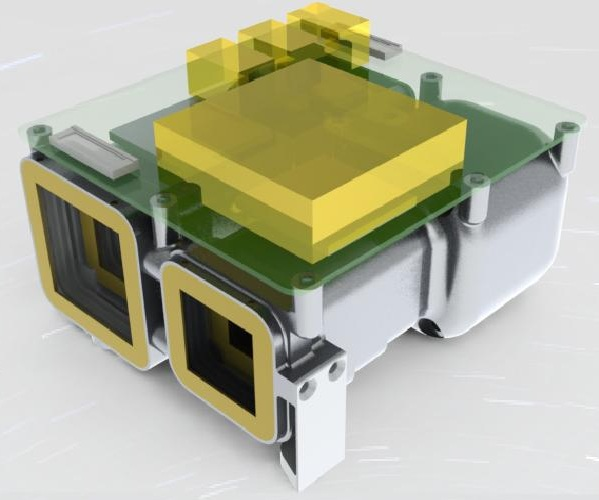
\includegraphics[width=0.7\linewidth]{images/EPD_Brochure}
\caption{}
\label{fig:epdbrochure}
\end{figure}
%\centering
%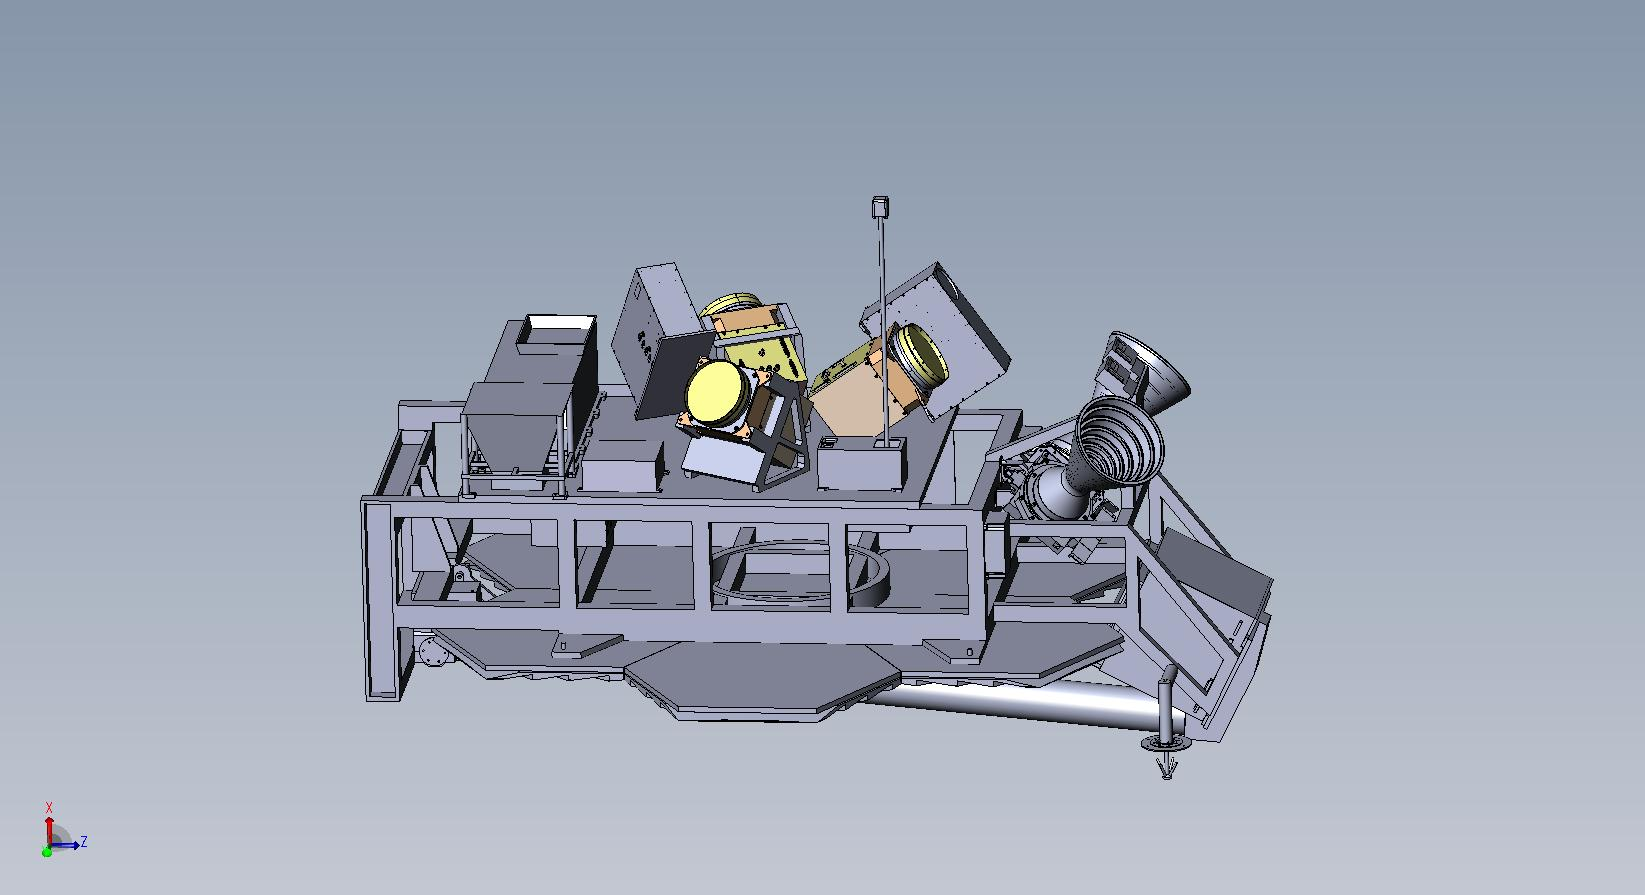
\includegraphics[width=0.8\linewidth]{images/lomonosov2}
%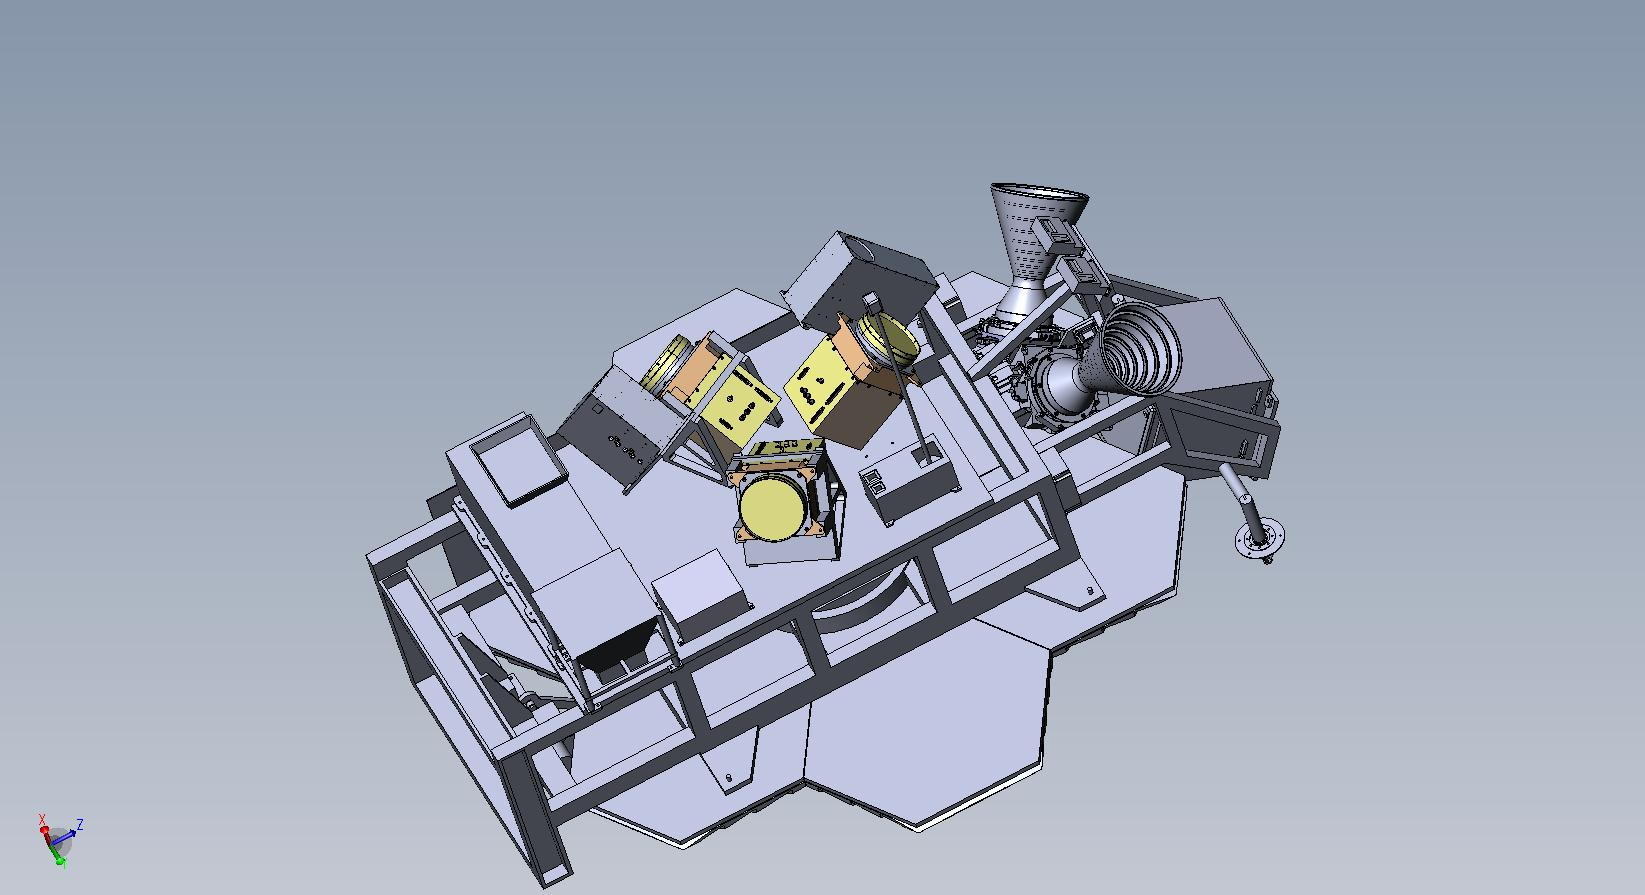
\includegraphics[width=0.8\linewidth]{images/lomonosov1}
%\caption{Внешний вид спутника Ломоносов старый}
%\label{fig:lomonosov2}
%\end{figure}

\begin{figure}
\centering
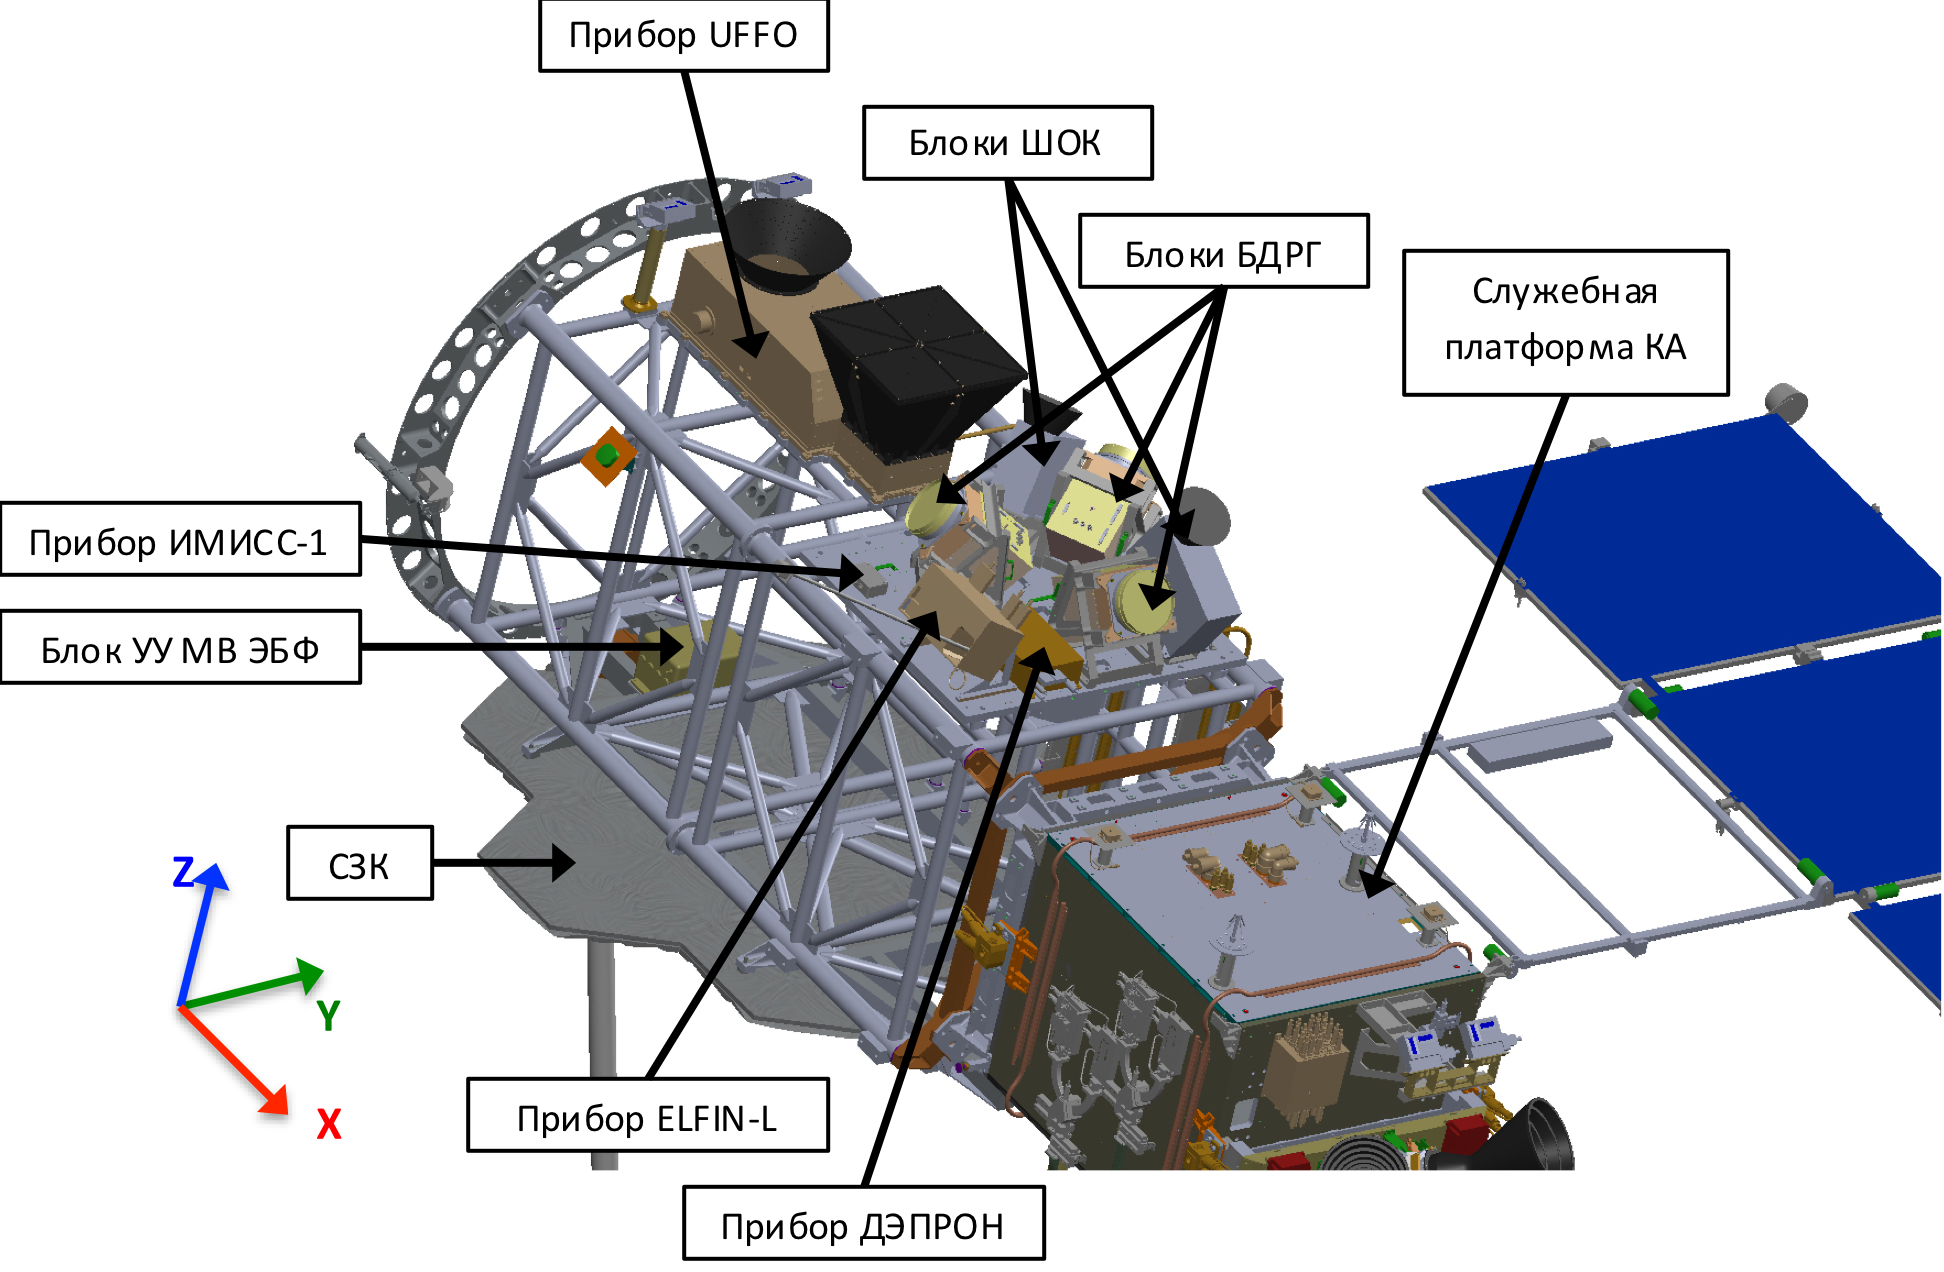
\includegraphics[width=0.9\linewidth]{images/lomo3}
\caption{Внешний вид спутника Ломоносов}
\label{fig:lomo3}
\end{figure}


           % Глава 1
%\chapter{Аппаратура для проведения исследований} \label{chapt2}

\section{Прибор Дэпрон}

Прибор Дэпрон разрабатывался как исследовательский инструмент для решения широкого круга научных задач. Основной задачей прибора является измерение мощности дозы и потоков ионизирующих излучений. Дополнительными задачами выделены регистрация нейтронов тепловых энергий и высокоэнергетичных частиц. Такое сочетание решаемых задач, для прибора относительно небольшого веса,  является уникальным и позволяет надеяться на получение достаточно подробной информации о радиационной обстановке на борту КА. 

\subsection{Устройство прибора}

В состав прибора ДЭПРОН входят два узла с полупроводниковыми детекторами и два узла с газоразрядными гелиевыми счетчиками нейтронов. Также в состав прибора входят узлы усиления и формирования сигналов от полупроводниковых и нейтронных детекторов и узел цифровой обработки сигналов.


Поглощенная доза регистрируется узлами с полупроводниковыми детекторами. Для получения информации о величине поглощенной дозы используется принцип регистрации величины заряда в объеме полупроводника, пропорционального энерговыделению в данном объеме. 

\begin{equation}\label{eq:benghin_doze}
D = \frac{E}{m} = \dfrac{w_i \cdot\dfrac{q}{e}}{m}
\end{equation}
где \begin{description}
	\item[$ D $] поглощенная доза
	\item[$ E $] энергия поглощенная в чувствительном объеме
	\item[$ m $] масса чувствительной зоны детектора
	\item[$ w_i $] энергия формирования np пары
	\item[$ e $] заряд электрона
	\item[$ q $] электрический заряд образованный в чувствительном объеме
\end{description}
Оба полупроводниковых детектора и скомпонованы в кассету и расположены в относительной близости друг от друга. Схема построения прибора с параллельным расположением двух полупроводниковых детекторов была использована для получения информации о ЛПЭ частиц, прошедших одновременно оба детектора. Спектр ЛПЭ зарегистрированных частиц позволяет вычислить эквивалентную дозу, используя постулированный в НРБ коэффициент качества ионизирующего излучения. Для перехода от поглощенной дозы в кремнии к эквивалентной дозе потребуется пересчет зарегистрированного спектра ЛПЭ в спектр ЛПЭ в воде, который произвадится умножением на коэффициент $ 1,21 $.
 Функциональная схема прибора ДЭПРОН показана на рисунке \ref{fig:Depron_blocksch}.
 
\begin{figure}
\centering
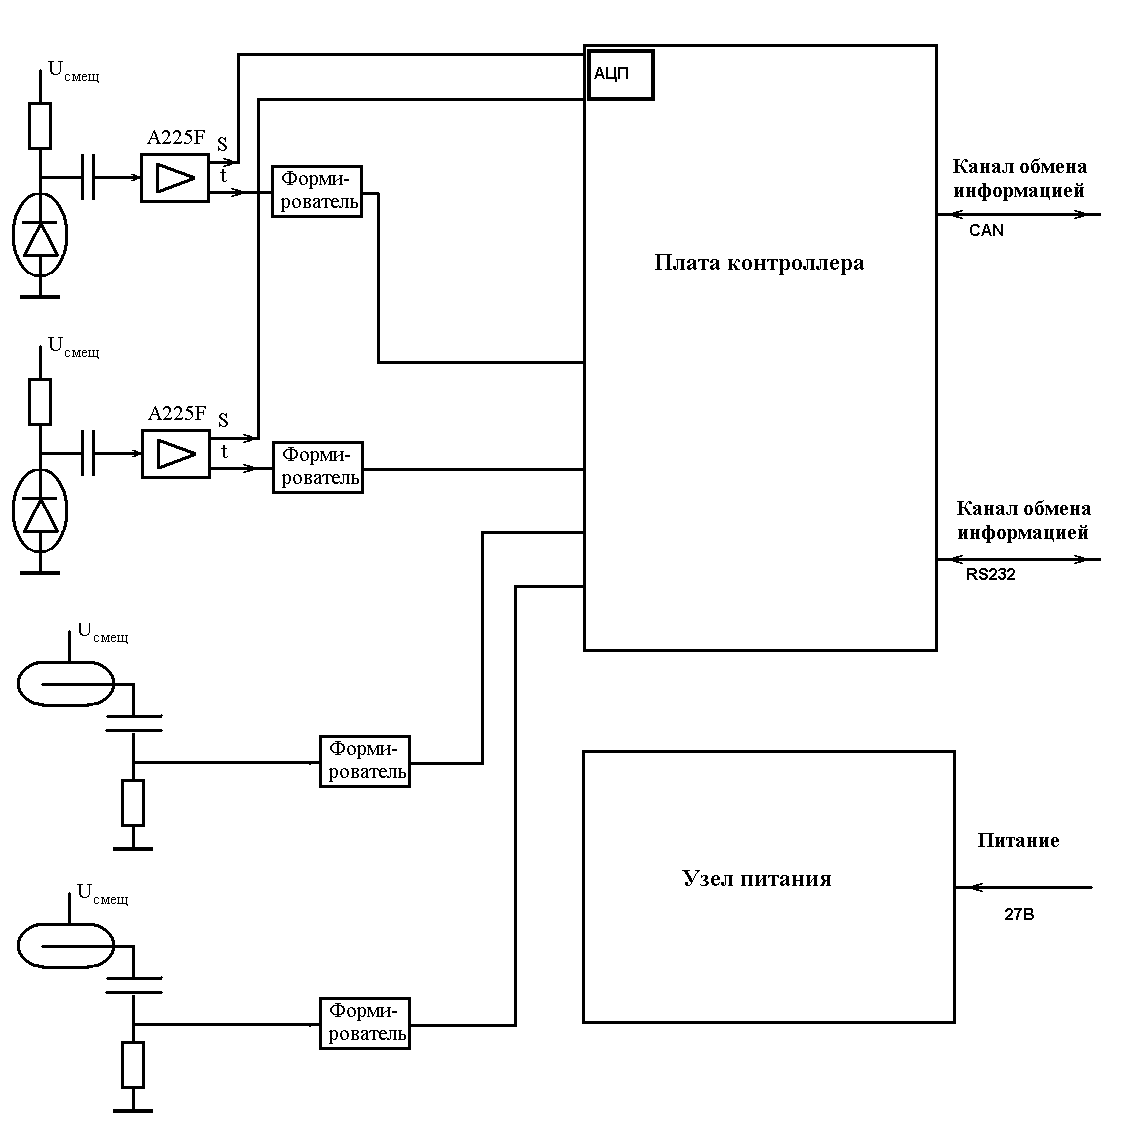
\includegraphics[width=0.8\linewidth]{images/Depron_blocksch}
\caption{Блок-схема прибора ДЭПРОН}
\label{fig:Depron_blocksch}
\end{figure}


%\newpage
%============================================================================================================================
\section{Конструктивные особенности прибора}

Прибор состоит из одного блока, габаритный чертеж которого представлен в Приложении 1. Габаритные размеры прибора: длина  280 мм, ширина 160 мм, высота 78 мм. Масса прибора - 3 кг. Корпус прибора составлен из шести пластин Д16т -- листового дюралюминия, толщиной 4,5 мм, обработанного на станке ЧПУ. В каждой пластине фрезерованы повторяющиеся выборки треугольной формы до толщины 2 мм. Выборки расположены таким образом, чтобы сформировать «ребра» жесткости в стенках прибора, как видно на рисунке \ref{fig:viborki}. С лицевой стороны пластины корпуса оксидированы, с целью получения электропроводной поверхности всего прибора.

\begin{figure}
\centering
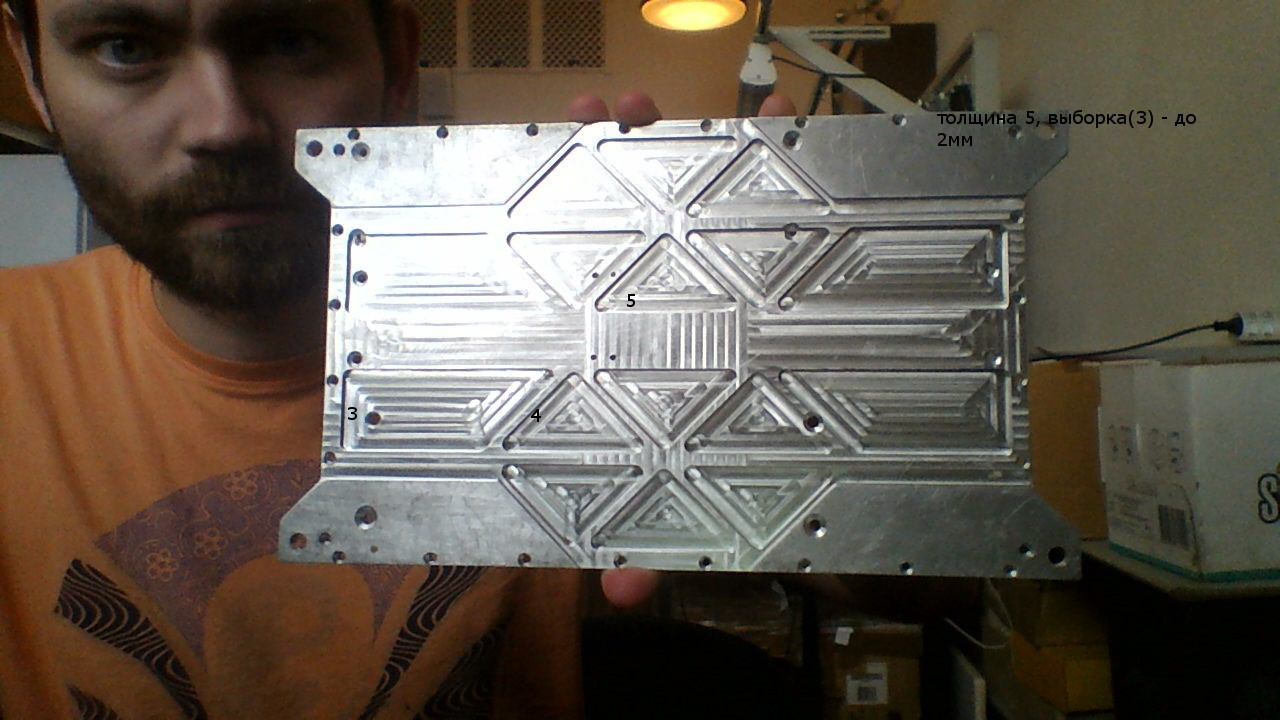
\includegraphics[width=0.7\linewidth]{images/viborki}
\caption{ Вариант размещения выборок в днище прибора ДЭПРОН.}
\medskip
{\small В последствии данный вариант переработан исходя из конструктивных соображений крепления модулей электроники и улучшения теплосброса источников питания, через термоконтакт с бортом КА. }
\label{fig:viborki}
\end{figure}


На лицевом торце прибора распложены два разъема СНП-333, используемых для передачи данных в БИ аппаратуры спутника (разъем Х1) и для передачи питания в прибор ДЭПРОН от бортовой аппаратуры спутника (разъем Х2). Также на лицевой панели находятся два разъема РС-7 предназначенные для передачи информации по каналу RS232 от прибора ИМИСС-1 (разъем Х5) и сквозной передачи питания от бортовой аппаратуры к прибору ИМИСС-1 (разъем Х4). Во всех перечисленных разъемах предусмотрен контроль стыковки разъемов с помощью короткозамкнутых линий, а также дублирование информационных и токонесущих линий.


Дополнительно на лицевую панель прибора вынесен технологический разъем РС 19 ХТ3, используемый для проверки функционирования прибора в лабораторных условиях методом подачи на детекторные узлы калиброванных сигналов с генератора, а также для контроля внутренних рабочих напряжений. Проверка работоспособности прибора и подача сигналов с генератора осуществляется с помощью  блока КПА, имеющему четыре экранированных канала для передачи низкоамплитудных сигналов и два светодиодных индикатора для контроля наличия рабочих напряжений  $ +5  $В и$  +12 $ В в приборе ДЭПРОН.  В штатном режиме работы данный разъем не подключен и закрыт заглушкой. Схема распределения линий в разъемах представлена в Приложении 2.

Платы электроники блоков усиления и формирования аналоговых сигналов располагаются в трех тонкостенных алюминиевых кассетах и выполнены в формате 11-ти контактных печатных плат размерами 34х50мм (\ref{fig:Depron_inside}). Данный формат печатных плат распространен в производстве научной аппаратуры изготовления НИИЯФ МГУ и с успехом применяется для космической аппаратуры уже на протяжении нескольких десятков лет. Применение данного стандарта позволяет соблюсти принцип модульности построения приборов, используя отработанные в космических условиях надежные схемы, компонуя из них тракты с параметрами, заданными потребностями текущих экспериментальных задач. 

\begin{figure}
\centering
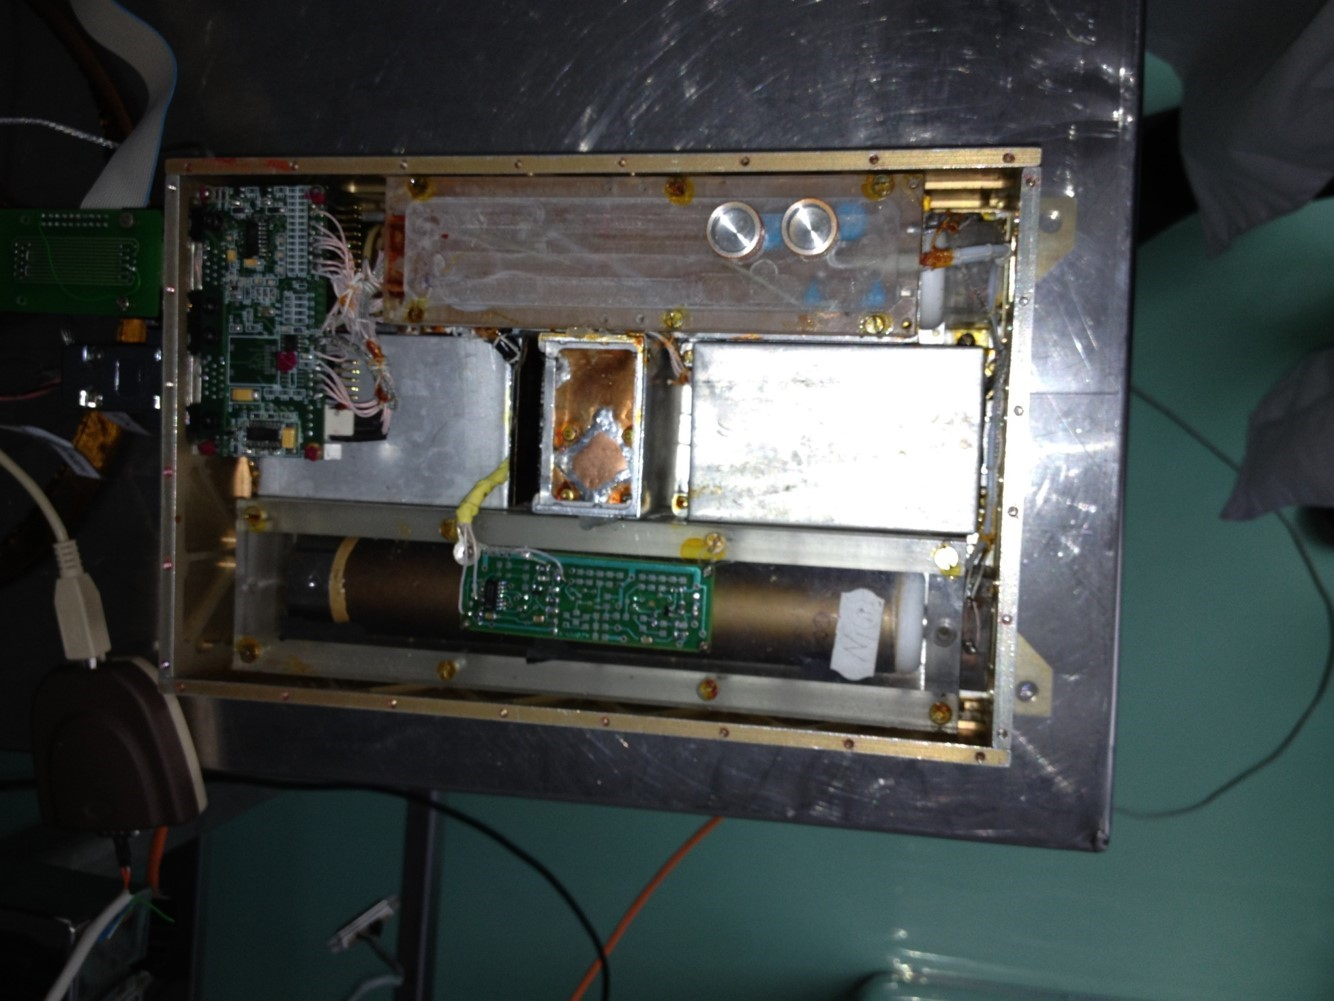
\includegraphics[width=0.7\linewidth]{images/Depron_inside}
\caption{Внутренняя компоновка модулей прибора ДЭПРОН. Вид сверху со снятой крышкой прибора.}
\label{fig:Depron_inside}
\end{figure}


В средней части рисунка последовательно располагаются три корпусных кассеты с платами электроники: левая и правая кассеты содержат платы формирователей триггерных сигналов от детекторов, центральная кассета ориентирована перпендикулярно и содержит две платы полупроводниковых детекторов и ЗЧУ, а также платы дополнительного усиления.

В нижней части рисунка находится нейтронный счетчик СИ13Н (циллиндр), экранированный 1 см оргстекла

\section{Детекторы}

Дозиметр заряженных частиц выполнен на кремниевых ионно-имплантированных Д1 пролетных детекторах, работающих в режиме регистрации амплитуд импульсов. Детекторы изготовлены по специальному заказу НИИЯФ МГУ в ООО «Детектор-СИ» в соответствии с АБЛК.418219.402ТУ. Данные детекторы предназначены для спектрометрии и радиометрии заряженных частиц в составе предназначенной для этих целей аппаратуры. Чувствительный элемент детектора изготовлен из высокоомного кремния n--типа по технологии ионной имплантации. Рекомендуемая схема включения детектора приведена на рисунке \ref{fig:detector_sch}. 


\begin{figure}[h]
	\centering
	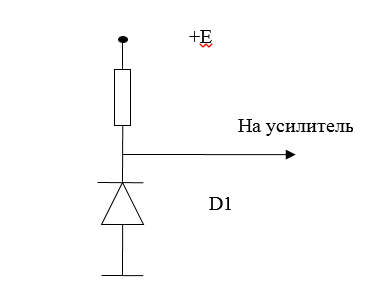
\includegraphics[width=0.5\linewidth]{images/detector_sch}
	\caption{Схема включения детектора.}
	\medskip
	\small
	\begin{description}
		\item[+Еп] источник напряжения;
		\item[Rсм] сопротивление смещения;
		\item[D1] Детектор.
	\end{description}			
	\label{fig:detector_sch}
\end{figure}
	


Детекторы могут эксплуатироваться при атмосферном давлении или в вакууме до 10\textsuperscript{-6} мм.рт.ст., таким образом подходят для расмещения в не герметичном корпусе прибора ДЭПРОН. Подробные значения параметров детекторов приведены в таблице \ref{tab:detectors}.

\begin{table} 

	\begin{tabular}{p{10cm}|cc}
		Наименование параметра&Фактические параметры\\ \hline
		Рабочее напряжение, В&90&\\ Обратный ток, нА&4\\
		Энергетический эквивалент шума, кэВ&5\\
		Постоянная времени квазигауссова формирования импульса, мкс&2\\
		Предельно допустимое напряжение, В&130\\
		\multicolumn{2}{l}{Примечания: Аттестация производилась при 26 C.}\\
		
	\end{tabular} 
	\caption{Полупроводниковые детекторы прибора ДЭПРОН (по материалам ТУ)}
		\label{tab:detectors}
\end{table}



\subsection{Телескоп детекторов}
В приборе Дэпрон  используются два полупроводниковых детектора. Детекторы образуют телескоп, то есть расположены параллельно на определенном расстоянии, что обеспечивает возможность регистрировать спектр ионизационных потерь.
Дополнительно использование двух детекторов позволяет повысить уровень надежности всего регистрирующего тракта.

Схематично относительное расположение детекторов показано на рисунке~\ref{fig:telescope}.  Расстояние между детекторами выбрано 18 мм, таким образом что телесный угол полета частиц, проходящих через оба детектора оказывается около 30 градусов. 


%\begin{tikzpicture}
%\draw[dashed,color=gray] (0,0) arc (-90:90:0.5 and 1.5);% right half of the left ellipse
%\draw[semithick] (0,0) -- (4,1);% bottom line
%\draw[semithick] (0,3) -- (4,2);% top line
%\draw[semithick] (0,0) arc (270:90:0.5 and 1.5);% left half of the left ellipse
%\draw[semithick] (4,1.5) ellipse (0.166 and 0.5);% right ellipse
%\draw (-1,1.5) node {$\varnothing d_1$};
%\draw (3.3,1.5) node {$\varnothing d_2$};
%\draw[|-,semithick] (0,-0.5) -- (4,-0.5);
%\draw[|->,semithick] (4,-0.5) -- (4.5,-0.5);
%\draw (0,-1) node {$x=0$};
%\draw (4,-1) node {$x=l$};
%\end{tikzpicture}



\begin{figure}	
	\centering
	\begin{tikzpicture}[scale=2, transform shape]
	\pic [fill=magenta, text=blue, draw=blue] at (5,0) {annotated cuboid={width=10, height=0.3, depth=10, units=мм}};
	\pic [fill=green, text=green!50!black, draw=green!25!black] at (5,-1.8) {annotated cuboid={width=10, height=0.3, depth=10, units=мм}};
	
	\draw[|->,semithick] (7,-1.8) -- (7,0);
	\draw (8,-1.8) node {$z=0$};
	\draw (8,0) node {$z=18$};
	%	\pic at (1,-3) {annotated cuboid={width=150, height=200, depth=250, scale=.01, units=m}};
	%	\pic [fill=cyan, text=blue!75!cyan, draw=blue!75!cyan] at (-3,-2) {annotated cuboid={width=15, height=18, depth=13.5, units=}};
	\end{tikzpicture}
	\caption{Телескоп детекторов прибора ДЭПРОН, масштаб 1:2}
	\label{fig:telescope}
\end{figure}

\subsubsection{Расчет геометрического фактора телескопа}
В соответствии с работой :[Analytical derivation of the
geometric factor of a
particle detector having
circular or rectangular
geometry
G R Thomas and D M Willis
SRC, Radio and Space Research Station, Ditton Park,
Slough, SL3 9JX
MS received 12 October 1971, in revised form 18 November
1971 ] общий геометрический фактор можно вычислить исходя из соображений затенения одного детектора вторым, что для геометриии с прямоугольными детекторами дает:

\[ G = Z^2 \int_{-X_1}^{X_1} \int_{-Y_1}^{Y_1} 
			\int_{-X_2}^{X_2} \int_{-Y_2}^{Y_2}
			\frac{dx_1dy_1dx_2dy_2}{\left\lbrace Z^2 + (x_2-x_1)^2 + (y_2-y_1)^2\right\rbrace^2 }\]

Численный расчет в пакете Mathcad ( рисунок \ref{fig:mathcadGeomfactor}) дает в результате для нашего случая геометрический фактор 0.145, учитывая что геометрический фактор отдельного детектора равен $ 4\pi $ и мы имеем два идентичных детектора, так что удваиваем полученный результат. Поправочный коэффициент для энерговыделения в телескопе детекторов 0,043, он рассчитан по соотношению \ref{eq:lpe_koef}, где $ S_0 $ площадь чувствительной поверхности.
\begin{equation}\label{eq:lpe_koef}
 \xi = \frac{Z}{2 \pi S_0 } \cdot \int_{-X_1}^{X_1} \int_{-Y_1}^{Y_1} 
\int_{-X_2}^{X_2} \int_{-Y_2}^{Y_2}
\frac{dx_1dy_1dx_2dy_2}{\left\lbrace Z^2 + (x_2-x_1)^2 + (y_2-y_1)^2\right\rbrace^2 }^{\frac{3}{2}}
\end{equation}


\begin{figure}[h!]
\centering
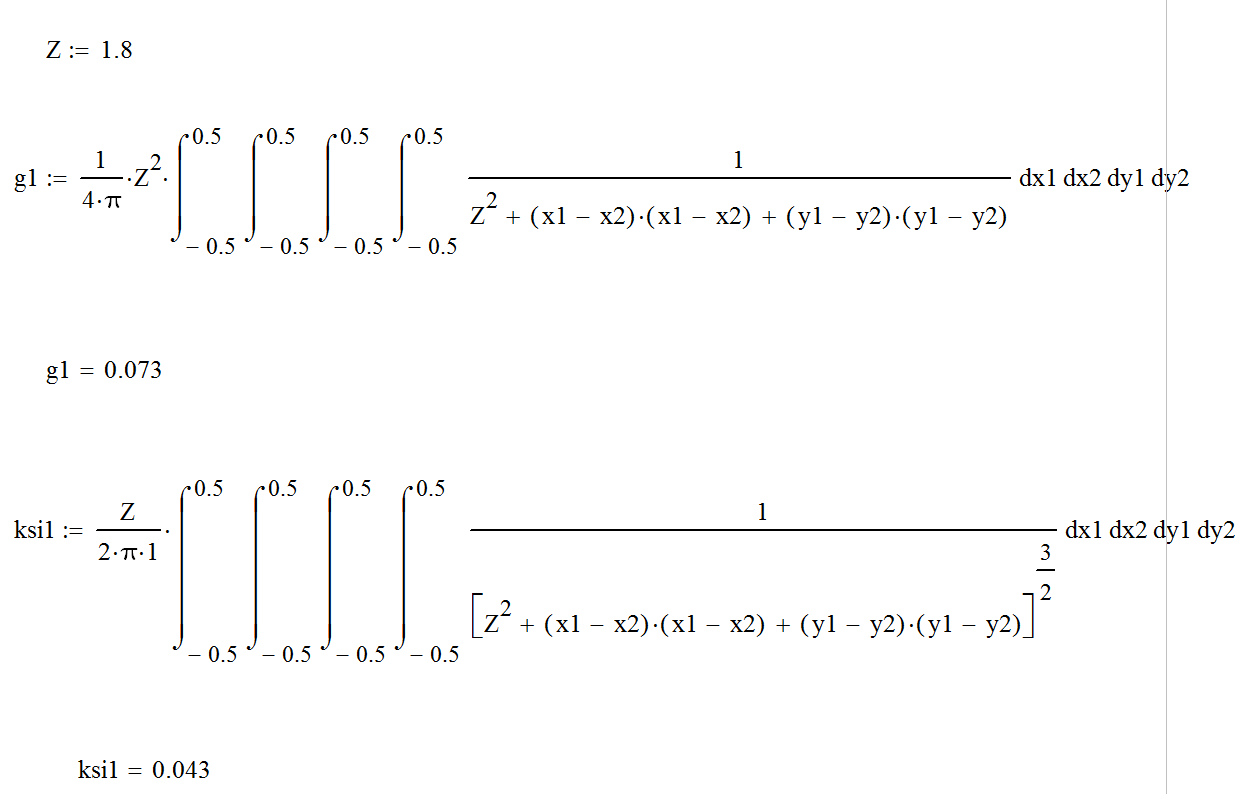
\includegraphics[width=0.7\linewidth]{images/mathcadGeomfactor}
\caption{ Расчет геометрического фактора телескопа в системе Mathcad}
\label{fig:mathcadGeomfactor}
\end{figure}

%\begin{figure}
%\centering
%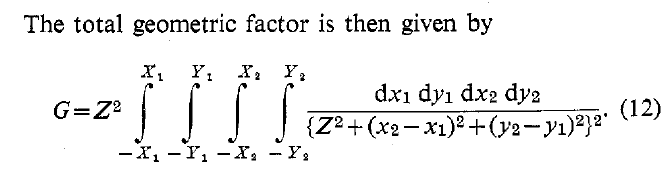
\includegraphics[width=0.7\linewidth]{images/totalgeomfactorintegral}
%\caption{}
%\label{fig:totalgeomfactorintegral}
%\end{figure}

%\begin{figure}
%\centering
%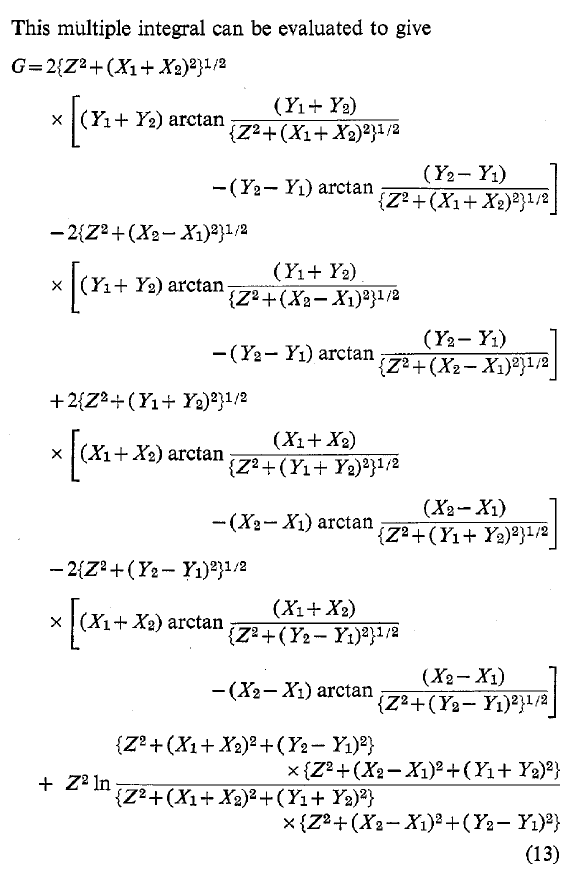
\includegraphics[width=0.7\linewidth]{images/totalgeomfactorsolved}
%\caption{}
%\label{fig:totalgeomfactorsolved}
%\end{figure}
%\begin{figure}
%\centering
%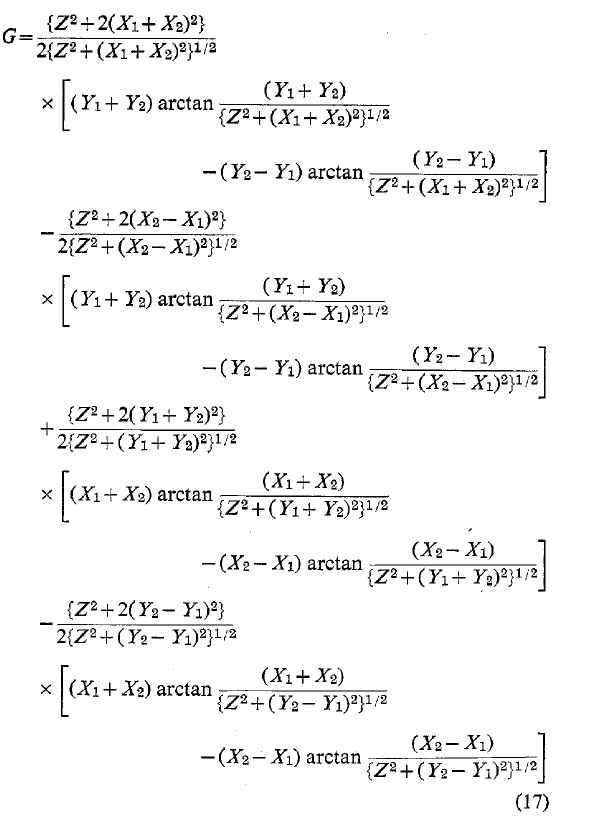
\includegraphics[width=0.7\linewidth]{images/totalgeomfactorsolved2}
%\caption[для интенсивности]{}
%\caption{}
%\label{fig:totalgeomfactorsolved2}
%\end{figure}


\subsubsection{Расчет энергетического коэффициента}
Детектор1: 3,4141 КэВ/канал 

Детектор2: 4 КэВ/канал - очень большой разброс по калибровкам - не могу понять почему:15.4 – 16.3 КэВ/канал. Необходимо найти исходные данные калибровок.

В ходе калибровок получено, что одной еденице по дозе детектора 1 соответствует 135 счетных имульсов в детектору 1, получается что умножив 135 на 3,4141  КэВ/канал  получаем энергетический эквивалент 3687 КэВ/(дозовый импульс) 

Так как мы имеем квадратный детектор с размерами 10мм * 10мм* 300мкм, оценим массу чувствительного объема детектора, подборав значения толщины тормозящего слоя вещества $ 0.0013 $ г/см$^2 $. Такая масса соответствует 5,58 мкм кремния или 1,04 см воздуха, а масса детектора соответственно: 0,0687г.

Дет1: 8,69пГр/кодАЦП 

Дет2: 9,32пГр/кодАЦП  

\todo{Далее можно посчитать на воду}

В программе микроконтроллера Дэпрон с целью сокращения передачи неинформативных каналов АЦП был сделан сдвиг на 3 разряда при записи в спектр энерговыделения, такая операция близка к операции деления на 8.

Независимый расчет дал результат для коэффициентов для первого детектора 0,0633  наноГрей/импульс, для второго -  0,0742 наноГрей/импульс. С учетом коэффициента 8 это близко к полученным результатам.

\subsection{Нейтронные детекторы}

Детектор нейтронов выполнен на счётчике медленных нейтронов «СИ-13Н», представляющем собой газоразрядный  счетчик, работающий в режиме коронного разряда. Для обеспечения надежности используются 2 счетчика. Второй детектор нейтронов окружен замедляющей оболочной из поликарбоната, что позволило расширить энергетический диапазон регистрируемых нейтронов. При прохождении нейтрона через газ Не-3, наполняющий счетчик, происходит ядерная реакция:
\[ n+^3\!He = p+T+764 \textrm{ КэВ}\]

Продукты реакции вызывают ионизацию газа в счётчике, что приводит к образованию газового разряда и появлению электрического импульса на электроде счетчика. Импульс поступает на вход усилителя-формирователя и, затем, поступает на регистр прерываний процессора, где используется для подсчета числа зарегистрированных нейтронов.

%\newpage
%============================================================================================================================
\section{Аналоговая обработка сигналов}

Платы полупроводниковых детекторов и предусилителей (внутренний номер SSD006) изготовлены методом фотолитографии в стандартном формате 34х50, использование современных миниатюрных электронных компонент позволило совместить блоки предусиления и детектирования на одной плате и закрыть единым экраном от электромагнитных помех.

Сигнал с полупроводникового детектора поступает на зарядовочувствительный предусилителя A225F, фирмы AMPTEC, специализирующейся на производстве компонент для космической промышленности. 

\todo{Рисунок A225F}

На выходах предусилителя формируются два сигнала. Один (S-сигнал) - имеет амплитуду пропорциональную заряду, образовавшемуся в детекторе и длительность порядка 5 -- 10 мксек. Этот сигнал поступает на амплитудно-цифровой преобразователь (АЦП). Второй сигнал предусилителя A225F (t-сигнал) имеет короткое, менее 0.5 мксек, время задержки от момента прихода сигнала с детектора до максимума амплитуды и используется для запуска процесса цифровой обработки пришедшего импульса. Этот (t-сигнал) сигнал поступает на вход усилителя и, после усиления, поступает на регистр прерываний процессора, где используется для запуска процесса преобразования амплитуды сигнала, поступившего на АЦП, в код. Дальнейшая обработка сигналов с полупроводниковых детекторов производится микропроцессором прибора в цифровой форме.

%\newpage
%============================================================================================================================
\section{Цифровая обработка сигналов}

Для записи результатов измерений прибора используется внутренняя память микроконтроллера, входящего в состав узла цифровой обработки сигналов. В нее записываются, а затем передаются в Блок Информации КА «Ломоносов» кадры информации.

На этапе опытно-конструкторских разработок (при макетировании прибора ДЭПРОН) в качестве узла цифровой обработки сигнала использовался 8-битный микроконтроллер ATmega128. Данная микросхема отличается низкой потребляемой мощностью и обладает развитыми средствами ввода данных и обмена информацией, а также достаточной вычислительной мощностью. Печатная плата контроллера была разработана в  НИИЯФ МГУ Н.Н. Веденькиным и Д.Г. Аксельродом. На плате расположены два АЦП, а также дополнительная память, независимый преобразователь питания и контроллер обеспечения связи по последовательному каналу (RS232). Как показали опытно-конструкторские работы, проведенные с макетом дозиметра ДЭПРОН, данный узел обеспечивает потребности по бортовой обработке сигналов от детектора по производительности, несмотря на то, что по современным меркам частота работы ядра процессора невелика - 16 MHz. Также выбранный контроллер обладает достаточным для поставленной задачи количеством входных каналов.

Для преобразования амплитуды импульсов, сформированных на выходе аналоговых трактов усиления, использовались 12-ти битные АЦП AD7495 фирмы Analog Devices со скоростью работы 1 MSPS (миллион измерений в секунду). Данные АЦП используют высокоскоростной последовательный интерфейс (SPI -- Serial Peripheral Interface), который был реализован программным способом. Управление моментом захвата амплитуды входного сигнала также производилось программным способом подачей цифрового сигнала «0» на линию CS. 
\begin{figure}
	\centering
	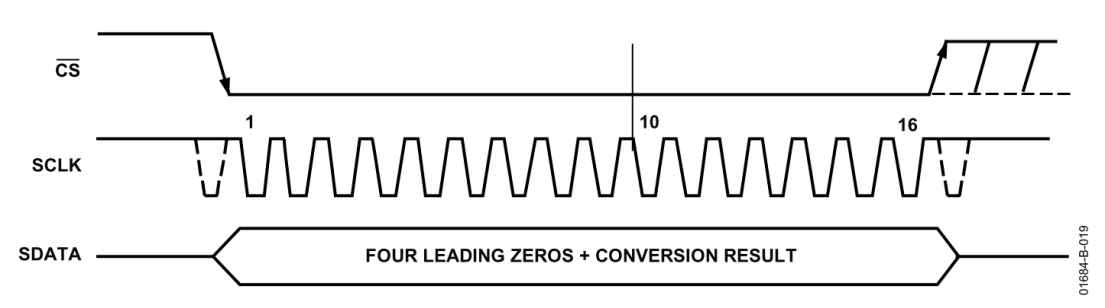
\includegraphics[width=0.7\linewidth]{images/adc}
	\caption{Использованный в приборе ДЭПРОН режим работы АЦП (AD7495), по материалам:  «1 MSPS,12-Bit ADCs  AD7475/AD7495», One Technology Way, P.O. Box 9106, Norwood, MA 02062-9106, U.S.A., 2005 Analog Devices, Inc.}
	\label{fig:adc}
\end{figure}

В первой версии платы цифровой обработки сигналов подключение обоих АЦП к контроллеру прибора производилось по независимым каналам: CS (Chip Select -- Активный логический вход АЦП), SCLK (Serial Clock -- логический вход АЦП), SDATA (Data Output -- логический выход АЦП). Задача максимально быстрого захвата сигналов с выхода предусилителя решалась включением встроенного в АЦП устройства выборки и хранения (англ. ``track and hold circuit'') в момент получения контроллером сигнала от таймингового выхода предусилителя. Для этого прерывания контроллера настроены при получении такого сигнала на выдачу управляющего сигнала на вход CS АЦП, ответственного за оцифровку сработавшего канала аналоговой части прибора. Дальнейшая оцифровка амплитуды захваченного в буфере АЦП сигнала производилась после выхода из процедуры обработки прерывания, так как этот процесс отнимает значительное время. Испытания процедуры управления оцифровкой АЦП показали, что точность измерений АЦП чувствительна к временной регулярности тактирующего сигнала подаваемого на SCLK АЦП. Одной из причин таких нерегулярностей является возможность срабатывания прерывания в ПО контроллера во время исполнения процедуры генерации тактирующих импульсов, что в условиях эксплуатации прибора при высоких потоках ионизирующих излучений (например, в области ЮАА) не редкость. Временное отключение обработки прерываний может устранить данный недостаток работы прибора, однако испытания такого режима работа показали накопление необработанных прерываний в буфере контроллера, которые впоследствии обрабатывались неверно, из-за чего решено отказаться от использования этого режима.


\todo{Рисунок. Осциллограмма: регулярность тактирующего сигнала, подающегося на SCLK АЦП.}

Выявление нерегулярности тактирующего сигнала потребовало проверку этого сигнала с помощью осциллографа. Дизассемблирование скомпилированного кода ПО микроконтроллера показало критические места кода, требующие изменения алгоритма генерации тактирующих импульсов и добавления промежутков простоя процессора (\texttt{\_nop} -- в коде ``no operation''). Окончательная проверка регулярности сигнала, генерируемого выверенным кодом, производилась снятием временной развертки тактирующего сигнала  на осциллографе. Данный подход использовался и при последующих отработках работы АЦП прибора ДЭПРОН.

\todo{Рисунок Блок схема подключения АЦП к контроллеру версия 1.}

Таким образом, в первой версии платы цифровой обработки сигналов использовались шесть независимых каналов контроллера, что ограничивало возможность подключения дополнительных информационных каналов с детекторной части прибора. Также одой из проблем данного подхода является двойная нагрузка на микроконтроллер прибора ДЭПРОН, так как управляющие сигналы генерируются программным способом. Такой подход предоставлял сомнительное преимущество в независимом управлении АЦП из программного обеспечения микроконтроллера, поэтому было принято решение изменения способа подключения АЦП.

Следующим конструктивным решением было включение обоих АЦП в параллельный режим работы, когда управляющий (CS) и тактирующий (SCLK) сигналы подаются на оба АЦП. Каналы данных (SDATA) подключены к независимым входам контроллера. 

\todo{Рисунок Блок схема подключения АЦП к контроллеру версия 2.}

При проектировании Блоков обработки Информации (БИ) было принято решение по организации обмена по каналу CAN между дочерними приборами, входящими в Комплекс Научной Аппаратуры (КНА) «Ломоносов». Однако использованный для макетирования контроллер ATmega128, и данный контроллер был заменен на AT90CAN128. Данное решение было продиктовано минимальными изменениями уже разработанного программного обеспечения и незначительными доработками печатных плат, необходимым для внедрения контроллера AT90CAN128.

Опыт работы с данным контроллером также показал его применимость для целей построения полноценного дозиметра ионизирующих излучений. Тем не менее, по требованию других участников проекта данный контроллер был заменен более современным и более производительным контроллером AT91SAM7X256. Всего в составе КНА насчитывается 4 прибора, в которых использована схема цифровой обработки сигнала на базе AT91SAM7X, некоторые из этих приборов испытывали нехватку производительности данного модуля до замены ЦПУ. В целях унификации разработанный аппаратуры модуль цифровой обработки сигналов и связи был заменен и в приборе ДЭПРОН. Данное изменение состава прибора повлекло за собой необходимость повторения цикла разработки программно-математического обеспечения прибора и проведения повторных калибровок АЦП и счетных каналов схемы цифровой обработки. Необходимость данных работ обусловлена принципиальным отличием архитектуры контроллера: в исходном варианте это архитектура AVR, а в окончательном ARM. 

В финальном варианте цифровая обработка сигналов осуществляется с помощью микропроцессора AT91SAM7X512. Программно-математическое обеспечение ДЭПРОН функционирует на одной микропроцессорной плате SSD234. Данная плата собрана на базе микроконтроллера AT91SAM7X512 производства фирмы ATMEL, и содержит процессор ARM7 TDMI® ARM® Thumb® с 32-разрядной RISC-архитектурой команд.

Программное обеспечение процессора осуществляет регистрацию сигналов, поступающих со схем преобразования импульсов с детекторов, их преобразование и накопление, передачу результатов по каналу связи с блоком информации КА. Объем сбрасываемой информации не превышает 1 Мбайт/сутки.

\section{Связь с внешними системами}
\emph{Связь с Блоком Информации «Ломоносов»}

Связь с БИ осуществляется посредством канала Controller Area Network (CAN), использующегося в качестве стандарта промышленных сетей. CAN ориентированн на объединение в единую сеть различных исполнительных устройств и датчиков. Режим передачи данных - последовательный, широковещательный, пакетный. Программные модули и аппаратные схемы разрабатывались для комплекса аппаратуры в целом Н.Н. Веденькиным и прошли проверку при доводке аппаратуры и комплексных испытаниях КНА.

Прибор ДЭПРОН формирует в рабочем режиме пакеты данных по 512 байт, которые накапливаются во внутренней памяти контроллера. Подготовленная очередь пакетов  передается на БИ КА «Ломоносов», где накапливается для передачи на Землю.

Передача информации от космического аппарата происходит через сеть фиксированной спутниковой связи. Данные передаются через общественную сеть Интернет и архивируются на специально выделенном сервере данных. Альтернативно, при отсутствии подключения к спутниковой сети связи, используется канал передачи телеметрической информации с платформы КА «Ломоносов», при таком подключении данные ДЭПРОН поступают на Землю через центр управления полетами (ЦУП) и ввиду ограниченной пропускной способности этого канала данные передаются частично.

\emph{Связь с прибором ИМИСС}

Связь с прибором ИМИСС-1 осуществляется по каналу RS232 (USART). Поступающая информация транслируется прибором ДЭПРОН в БИ по каналу CAN без изменений. В соответствии с расчетным объемом данных от прибора ИМИСС затраты производительности микроконтроллера ДЭПРОН на трансляцию данных в БИ будут незначительны по отношению к затратам на выполнение основных задач прибора ДЭПРОН.

\subsection{Питание}

Электропитание схем прибора ДЭПРОН осуществляется с использованием DC/DC преобразователей. Напряжение питание бортовой сети 27В, подключено через разъем Х2 прибора ДЭПРОН и поступает на два преобразователя 28/12 В. С первого преобразователя напряжение поступает на стабилизатор напряжения и далее из этого напряжения формируются номиналы: +6 В, для питания схем усилителей, формирователей и микропроцессора. Со второго преобразователя питание поступает на преобразователь +70 В, для питания полупроводниковых детекторов и на преобразователь +1200 В, для питания газоразрядных счетчиков. 

\subsection{Программное обеспечение}

Программно-математическое обеспечение прибора ДЭПРОН состоит из программы для контроллера прибора, написанной на языке C++(C), c использованием пакета IAR  Workbench\textsuperscript{®} для микроконтроллеров архитектуры ARM\textsuperscript{®}. 


Исполняемый код программы формируется из двух файлов: 


\begin{itemize}
	\item 	\texttt{detector.c} -- прикладные функции для работы прибора ДЭПРОН
	
	
	\item \texttt{main.cpp} -- инициализация контроллера прибора и функции обмена информацией с БИ. В процедуре main этого файла работает основной бесконечный цикл программы, в котором вызываются функции обмена информацией по каналу CAN и процедура \texttt{Detectors\_Handling}.
	
	
\end{itemize}
Работа прибора ДЭПРОН основана на прерываниях, которые обрабатываются по мере их поступления в процедуре \texttt{Ext\_Interrupt} (см. рисунок \ref{fig:ext_interrupt}), а ресурсоемкий разбор полученных данных и запуск АЦП происходят в процедуре \texttt{Detectors\_Handling}, которая отрабатывает постоянно. 

\begin{figure}
\centering
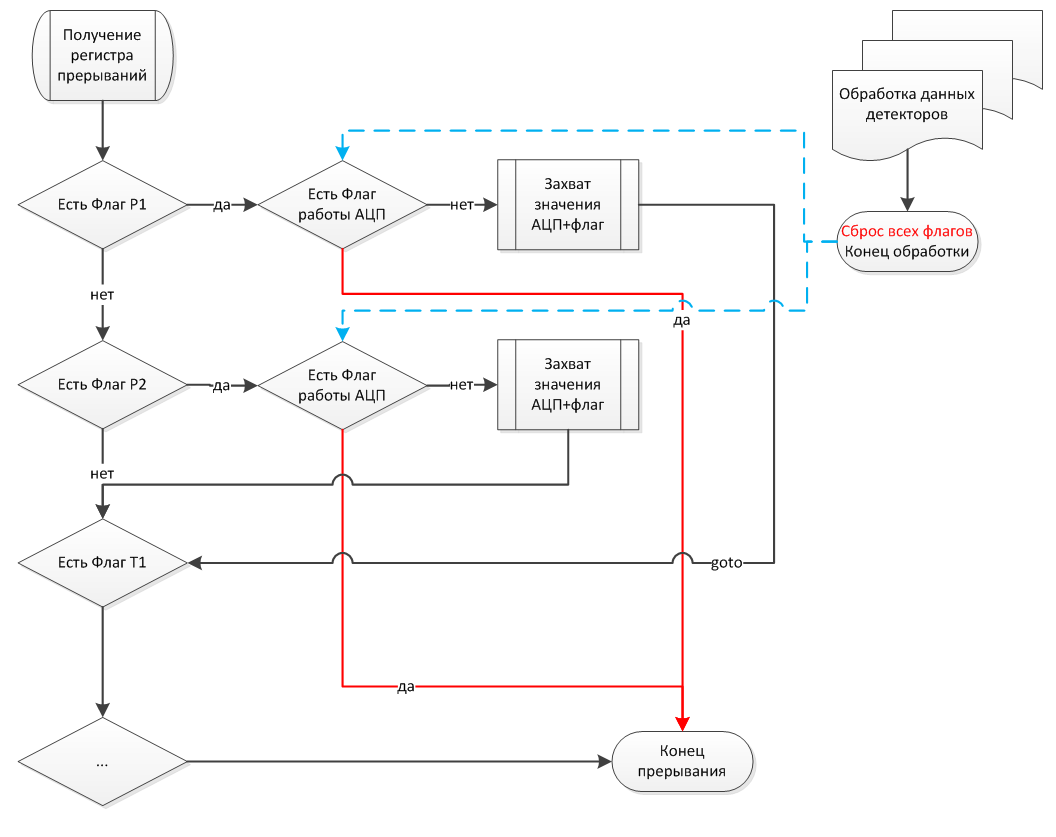
\includegraphics[width=0.7\linewidth]{images/ext_interrupt}
\caption{Блок схема работы процедуры \texttt{Ext\_Interrupt}, \todo{требует обновления!}}
\label{fig:ext_interrupt}
\end{figure}



\todo{Таблица Распределение битов в регистре прерывания}

\todo{Блок схема работы процедуры Detectors\_Handling}


\subsection{Контрольная проверочная аппаратура}

Контрольно приемная аппаратура (КПА) прибора ДЭПРОН используется для  проведения автономных испытаний прибора. КПА ДЭПРОН состоит из:


\begin{itemize}
	\item 	Ноутбук (или другой персональный компьютер) с установленной операционной системой Windows XP и установленным специальным программным обеспечением (программой Depron Terminal), наличием порта RS232, либо дополнительно преобразователь интерфейсов USBRS232;
	
	
	\item 	Блока питания, обеспечивающего измерение потребляемого тока нагрузки GwINSTEK GPS-4303;
	
	
	\item 	Преобразователя интерфейсов USBRS232 (при отсутствии COM порта у ПК);
	
	
	\item 	Комплекта соединительных кабелей 
	
	
	\item 	Блока КП -- контрольно-приемного блока
	
	
\end{itemize}






\todo{Рис.1. Схема подключения КПА для проверки функционирования прибора ДЭПРОН.}


Блок КП предназначен для подключения генератора и осциллографа к тестовым входам прибора ДЭПРОН, а также для контроля наличия рабочих напряжений в контурах прибора. Блок КП имеет 4 входных гнезда BNC промаркированных в соответствии с каналами прибора ДЭПРОН на которые передаются тестовые сигналы с генератора: 



\begin{itemize}
	
	\item 	X1	
	
	\item 	X2\ldots
		
\end{itemize}

На лицевой панели блока КП расположены 2 светодиодных индикатора. Подключение Блока КП к прибору ДЭПРОН происходит через тестовый вход XT3 (типа РС19).


\section{Градуировочные  характеристики прибора}
Градуировка прибора ДЭПРОН проводится с использованием зависимости \ref{eq:benghin_doze_code}

\begin{equation}\label{eq:benghin_doze_code}
D = \frac{E}{m} = \dfrac{w_i \cdot\frac{q}{e}}{m} = \frac{w_i \cdot \Delta U \cdot\sum K \cdot C}{m \cdot e \cdot \eta}  = V \cdot \sum K
\end{equation}
по материалам  «ПРИБОР ДЭПРОН, В.В. Бенгин, О.Ю. Нечаев, И.А. Брильков, А. Амелюшкин, В. Петров»  представленной на рабочем совещании «Universat» (Университетские спутники), 7-10 июня в МГУ им. М.В. Ломоносова

где \begin{description}	
	\item[$ K $] выходной сигнал АЦП
	\item[$ C $] входная емкость системы детектор-предусилитель
	\item[$ \eta $] суммарный градуировочный коэффициент тракта усиления до АЦП
	\item[$ \Delta U $] шаг дискретизации АЦП
\end{description} 
Большая часть величин в этой формуле известна, а экспериментально были определены недостающие величины. Данная работа была проведена Сиолаповым Виктором вместе с Бенгиным В.В, 
           % Глава 2
%\chapter{Обработка информации с прибора} \label{chapt3}


Отладка программного обеспечения и проверка обработки сигналов от детекторов на этапе  конструкторских работ производилась подключением канала RS232 к последовательному (COM) порту персонального компьютера. Программное обеспечение контроллера формирует отладочные посылки и массивы тестовых данных и отправляет по интерфейсу USART, реализованному на всех использовавшихся контроллерах. Такой способ передачи тестовых данных выбран как максимально приближенный к условиям реального функционирования прибора. 

Автономные испытания Дэпрон проходили с момента создания первых версий ПМО до ноября 2011. В ходе этих испытаний были проведены основные калибровки усилительных трактов прибора с помошью генератора сигналов и с помошью  источников ионизирующего излучения.

Отработка работы прибора в комплексе научной аппаратуры позволяет использовать штатный способ передачи информации по каналу CAN, в таком случае критерием работы прибора является выдача от БИ содержательных блоков информации с меткой, соответствующей прибору ДЭПРОН. 

\section{Схема обработки информации при КДИ}\label{sec3.1}

Для обработки данных и отладки работы прибора ДЭПРОН были использованы специально разработанные программные средства. Поскольку отладка прибора ДЭПРОН производится подключением по каналу RS232 а при работе в штатном режиме передача данных ведется по каналу CAN, для взаимодействия с прибором были написаны две различные программы.

\subsection{Отладочная программа Depron Terminal}

Данная программа предназначена для отладки прибора во время лабораторных испытаний, проверки работоспособности прибора при приемо-сдаточных работах. Программа была написана в средстве разработки ПО Microsoft Visual Studio на языке C\#, c использованием фрэймворка .NET3.5. Пользовательский интерфейс программы построен на основе WinForms, поэтому отличается консервативностью и достаточно низкими аппаратными требованиями.

Программа позволяет:


\begin{itemize}
	\item 	Подключаться к прибору ДЭПРОН по каналу RS232 (с использованием COM порта)
	
	
	\item 	Принимать и отображать тестовые данные сформированные прибором ДЭПРОН
	
	
	\item 	Сохранять запись потока данных на жесткий диск ПК (в фоновом режиме и по запросу)
	
	
	\item 	Открывать сохраненные данные с носителя информации
	
	
	\item 	Посылать команды на прибор ДЭПРОН (в том числе с заданной периодичностью)
	
	
\end{itemize}
\begin{figure}
\centering
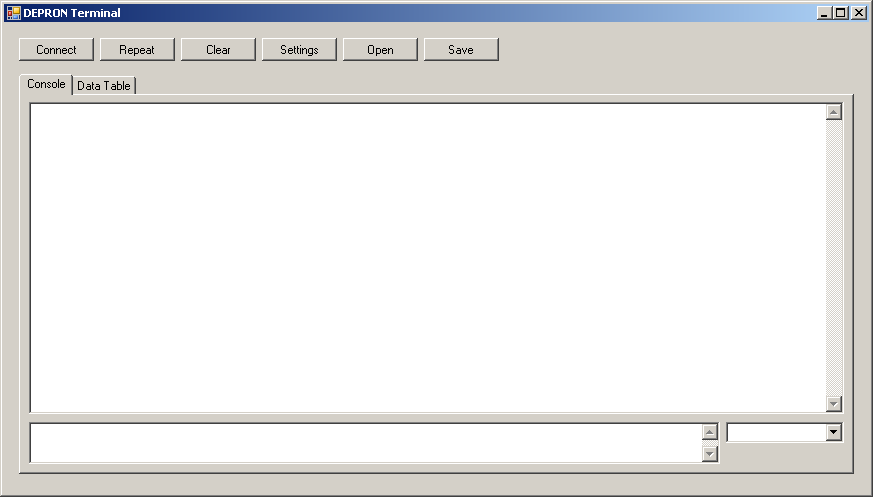
\includegraphics[width=0.7\linewidth]{images/depron_terminal}
\caption{Интерфейс программы \textbf{Depron Terminal}}
\label{fig:depron_terminal}
\end{figure}

Данная программа была использована как основа для разработки отладочной программы для дозиметрических блоков ДБ-8м. Основные принципы работы новой программы, названной \textbf{DB8m Terminal} были сохранены и она обеспечивает те же базовые функции. Дополнительно программа обеспечивает возможность накопления спектров энерговыделения по детекторам ДБ-8м и отображения их в графическом виде, в режиме реального времени. 
\begin{figure}
\centering
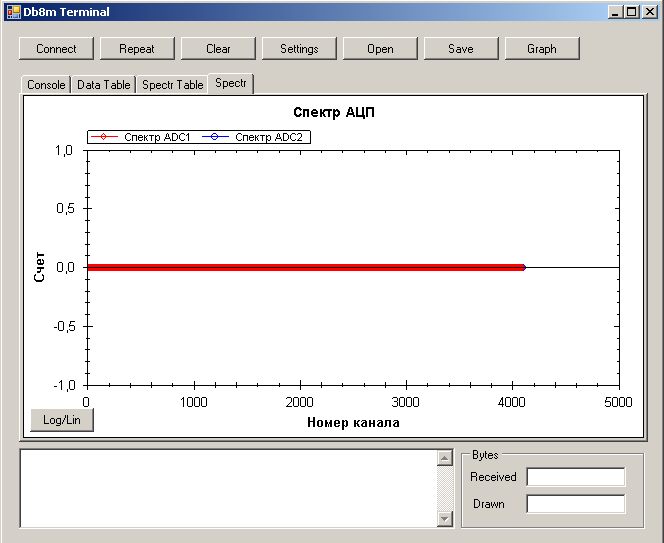
\includegraphics[width=0.7\linewidth]{images/db8m_terminal}
\caption{Интерфейс программы \textbf{DB8mTerminal}}
\label{fig:db8m_terminal}
\end{figure}

Графическое отображение спектров реализовано с использованием компонента ZedGraph. Введение такой возможности значительно ускорило калибровку и градуировку прибора на источниках радиационного излучения, так что может быть рекомендовано для программ аналогичной направленности.

\subsection{Программа DepronExplorerView}

Данная программа предназначена для просмотра и обработки данных прибора полученных во время комплексных испытаний или во время штатной работы прибора. Аналогично Depron Terminal, данная программа была написана в средстве разработки ПО Microsoft Visual Studio на языке c\# c использованием фрэймворка .NET3.5. Пользовательский интерфейс программы построен на основе WPF.


На момент комплексных испытаний прибора ДЭПРОН программа DepronExplorerView позволяет отображать все типы бинарных данных, полученных от прибора ДЭПРОН, в таблично-текстовой форме и сохранять полученные данные в текстовые файлы. Для удобства использования интерфейс программы выполнен в стиле файлового менеджера. 

Подготовленная программа активно использовлалась при всех испытаниях прибора ДЭПРОН в комплексе аппаратуры спутника, а также будет использоваться при предполетных проверках на космодроме Восточный.

\begin{figure}
\centering
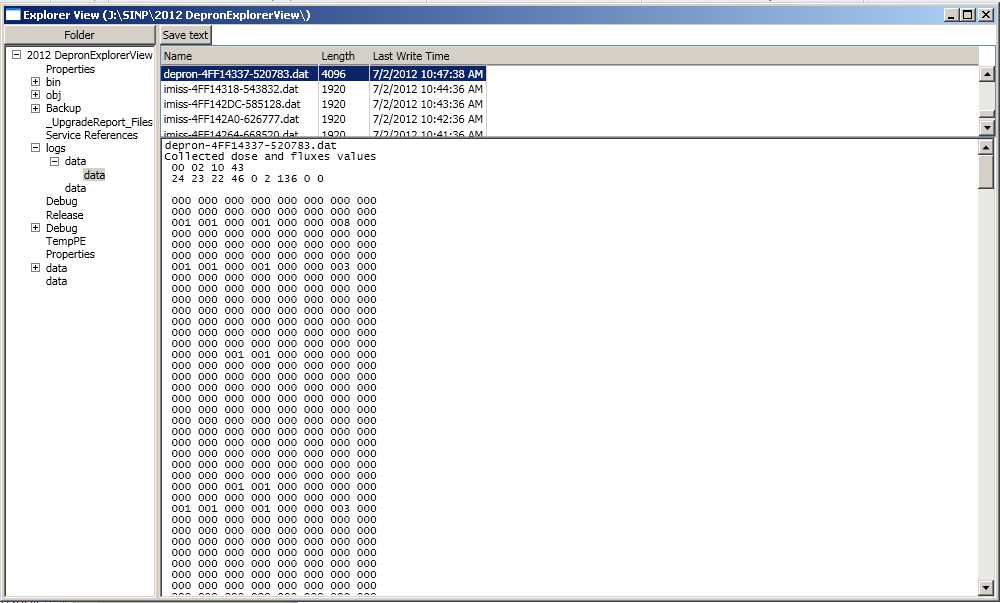
\includegraphics[width=0.8\linewidth]{images/depron_explorer}
\caption{Интерфейс программы \textbf{DepronExplorerView}}
\label{fig:depron_explorer}
\end{figure}


\subsection{Структура массивов (базы данных) результатов измерений}

Результаты измерений прибора ДЭПРОН формируется в массивы информации размером 512 байт.


Каждое сообщение состоит из следующих полей:

\begin{itemize}
	\item  начало сообщения;

	\item  категория;

	\item  длина сообщения;

	\item  данные.
\end{itemize}


Поле {``}начало сообщения'' содержит 2 байта:
\begin{itemize}
	\item байт DLE -- 11110000;
	\item байт STX -- 11111111.
\end{itemize}


На момент написания в программе ДЭПРОН используются нестандартные значения для байт DLE и STX, поэтому во избежание путаницы в дальнейших версия ПО ДЭПРОН будут использоваться общепринятые значения этих байт.


Поле ``категория'' состоит из одного байта (CAT). При обмене с БИ используются варианты сообщений: A, S, H, N. Коды сообщений соответствуют таблице ASCII: A - 01000001, S - 01010011, H - 01001000, N -- 01001110.

Поле ``длина сообщения'' содержит 1 байт (LEN) по умолчанию передается ``\ensuremath{\backslash 0}'', что означает общую длину посылки 512 байт.


В ином случае значение длины равно общему числу байт сообщения, исключая поле ``начало сообщения''.


Поле ``данные'' (RECORD) содержит данные в соответствии с описанием передаваемых сообщений и их спецификацией.



Общая структура сообщений выглядит следующим образом:

\begin{tabular}{|p{4.5cm}|c|c|p{2.5cm}|}
	\hline
	Начало сообщения (DLE,STX) & Категория(CAT) & Длина(LEN)  & Данные (RECORD) \\ \hline
	Метка 1                    & \multicolumn{2}{c|}{Метка 2} &  \\ \hline
	2 байта                    & \multicolumn{2}{c|}{2 байта} & {508 байт  }    \\ \hline
\end{tabular}

 
\subsection{Содержание блоков данных ДЭПРОН}

Прибор ДЭПРОН в процессе штатной работы формирует несколько типов массивов информации, которые соответствуют различным типам измерений:


\begin{itemize}
	\item 	дозиметрические измерения потока ионизирующих излучений;
	
	
	\item 	измерения спектров потока ионизирующих излучений;
	
	
	\item 	запись данных высокоэнергетичных событий в детекторах;
	
	
	\item 	измерение временного характера кратковременных нейтронных явлений;
	
	
\end{itemize}
Также прибор ДЭПРОН формирует ответ на пришедшую команду от БИ.





Типы массивов данных прибора ДЭПРОН:


\begin{itemize}
	\item 	блок данных ДЭПРОН  A  		Collected dose and fluxes values
	
	
	\item 	блок данных ДЭПРОН  S 		Energy deposition spectra
	
	
	\item 	блок данных ДЭПРОН  H  		High Amplitude Data
	
	
	\item 	блок данных ДЭПРОН  N		Neutron burst data
	
	
	\item 	блок данных ДЭПРОН  Т		квитанция на полученную команду
	

\end{itemize}

\subsection{Периодичность выдачи массивов данных}
\begin{center}
	{\small 
		\begin{tabularx}{\textwidth}{|c|c|X|}
			\hline
			Блок данных & Содержание                                 & Периодичность \\ \hline
			     A      & Величины поглощенной дозы и потоков частиц & 1 мин. \\ \hline
			     S      & Спектр энерговыделения                     & 5 мин. \\ \hline
			     H      & Данные о высокоэнергетичных событиях       & По мере накопления данных \\ \hline
			     N      & Данные по нейтронным вспышкам              &  По мере накопления данных, но не более 10 массивов в минуту\\ \hline
			     T      & Квитанция на полученную команду            &  По мере поступления команд\\ \hline
		\end{tabularx}
}
\end{center}



\section{Обработка наземных данных}\label{sec3.2.1}
В процессе наземных отработок прибор ДЭПРОН включался автономно при калибровке и в процессе проведения испытаний в комплексе аппаратуры.


В конце 2011 года прибор был передан на отработку в комплексе научной аппаратуры и далее работа с ним происходила по штатному каналу

Включения на стенде космодрома Восточный проходили  
2016-03-13,
2016-03-14,
2016-03-15,
2016-03-16.


В результате обработки данных, полученных в результате включений прибора ДЭПРОН на стенде космодрома ВОСТОЧНЫЙ, подтверждено прибор работает в штатном режиме и регистрирует естественный радиационный фон помещения.
В данных присутствуют массивы информации по величинам поглощенной дозы и потоков частиц, и спектры энерговыделения в детекторах прибора, состав массивов соответствует разработанному протоколу обмена. Эти массивы выдаются прибором, в соответствии с заданной периодичностью – 1 и 5 минут соответственно. Два дополнительных блока данных не выдаются прибором до заполнения массивов высокоэнергетичных событий и нейтронных всплесков, которые в условиях естественного радиационного фона на Земле не встречаются.

По данным в блоках A фоновый счет в п/п детекторе 1 - 108 частиц за 4 часа, и в детекторе 2 -90, за тот же временной промежуток. Счет в детекторе нейтронов 2 – 38, в детекторе 1 – 12 частиц за промежуток 4  часа.

%\todo{обработать наземные данные}

\section{Схема обработки и распределения потоков информации полетных данных}\label{sec3.2}
\subsection{Восстановление метки времени в массивах данных}
В процессе обработки данных полученных во время летных испытаний прибора ДЭПРОН 
было выяснено, что во временных метках массивов информации имеются ошибочные 
значения, происхождение которых связано с отсутствием календаря в ПО 
микроконтроллера ДЭПРОН. Так как в ПО не были заложены длительности месяцов 
года, при наступлении нового месяца метки времени продолжают приходить с 
номером предыдущего месяца к числу дней прибавляется дополнительный и возникают 
ошибочные даты: 2016-05-32 и 2016-05-33. На рисунке 
\ref{fig:deprontimedifference} видно наличие пробелов при наступлении нового 
месяца, так как невозможно автоматическое распознание меток времени. Наличие 
таких отклонений должно быть 
исправлено отправлением метки времени в прибор от БИ в первую минуту нового 
месяца. Однако пока такая процедура не проводилась был накоплен значительный 
объем измерений и для их верной привязки к действительным датам был разработан 
алгоритм и реализован на языке R, листинг кода представлен в \ref{list:datecor}.

\begin{figure}
	\centering
	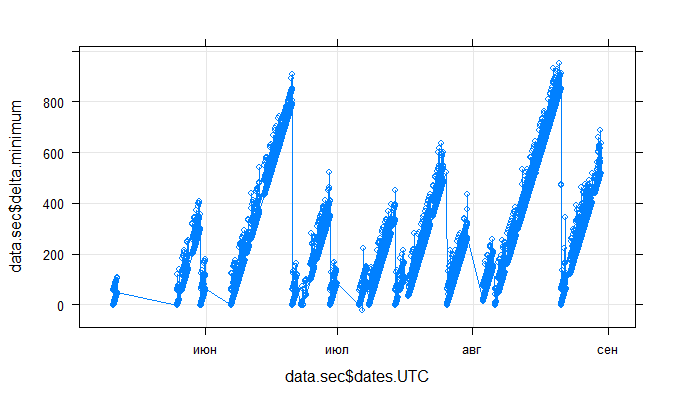
\includegraphics[width=0.9\linewidth]{images/deprontimedifference}
	\caption[Временной ряд разницы приборного времени и меток начала записи в 
	файл.]{Временной ряд разницы приборного времени и меток начала записи в 
		файл. Показаны первые шесть месяцев после запуска спутника Ломоносов, 
		отключения прибора соответствуют циклограмме летных испытаний, а 
		пробелы в данных в начале месяца соответствуют ошибочным номерам дня в 
		месяце.}
	\label{fig:deprontimedifference}
\end{figure}

При привязке секундных данных к баллистическим данным была обнаружена еще одна 
проблема с метками времени в данных 
ДЭПРОН, связанная с постоянным уходом приборных часов. Для решения этой 
проблемы также был разработан алгоритм \ref{list:timecor} и успешно применен 
для восстановления меток времени 

\subsubsection{Описание алгоритма восстановления дат}

На первом этапе  бинарные данные каждого сброса распаковываются в текстовый вид 
с получением таблицы с колонками: \texttt{YYYY-MM-DD hh:mm:ss-1s,	count.h,	
count1,	count2,	count.both,	n1,	n2,	dose1, dose2,	filename,	timestamp}. 
Далее осуществляется разделение текстового поля с меткой времени --- 
\texttt{YYYY-MM-DD hh:mm:ss-1s} на дату и время, а после полученное поле 
\texttt{date} на год, месяц и день - обозначенные \texttt{year, month, day} 
соотвественно.

Создается поле \texttt{dates} имеющее тип данных \texttt{ISOdate} исходя только 
из полей даты года и месяца, а день месяца устанавливается первый. Далее к полю 
\texttt{dates} 
добавляется число дней из поля \texttt{day}, минус один день. В последнюю 
очередь в поле \texttt{dates} выставляется приборное время, отделенное в начале 
алгоритма.

\subsubsection{Описание алгоритма восстановления метки времени}

Приборное время ДЭПРОН установлено на третий часовой пояс и соотвествует 
Московскому 
времени, поэтому для унификации базы данных получено поле \texttt{dates.UTC} 
соответствующее приборному времени смещенному на 3 часа.



Далее в результате ручного анализа данных было найдено что за сутки внутренние 
часы ДЭПРОН уходят вперед на 57 секунд, что хорошо видно на графике~
\ref{fig:deprontimedifference} поэтому был введена поправка \texttt{kt}:
\[ kt = (56.77315002) /86400 \]
Далее c использованием полученной поправки из времени UTC получено 
скорректированное приборное время, хотя это время смещено отностительно 
действительного всемирного времени это смещение меняется каждый раз при 
выключениях прибора в ходе программы исследований \ref{fig:deprontimeplot}. 

\begin{figure}
	\centering
	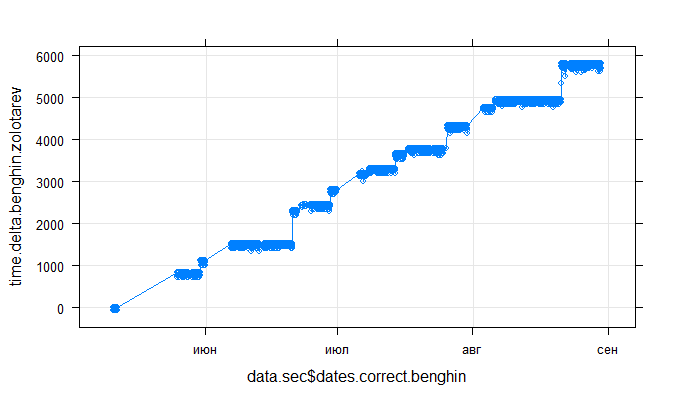
\includegraphics[width=0.9\linewidth]{images/deprontimeplot}
	\caption[Временной ряд разницы калиброванного приборного времени и меток 
	начала записи в файл.]{Временной ряд разницы калиброванного приборного 
	времени и меток начала записи в файл.}
	\label{fig:deprontimeplot}
\end{figure}


Для автоматического определения этого смещения необходимо привязать его к 
независимому источнику точного времени - в качестве такого рассмотрены метки 
времени начала записи в бинарный файл данных БИ а также метки окончания записи 
файловой системы. Оказалось что разница времени меток последней записи сильно 
разнится относительно всех других меток, видимо по причине буферизации записи в 
файл данных, поэтому в качестве реперного времени выбрано время создания файла, 
которое записано в названии каждого файла как POSIXtime в виде 
шестнадцатеричного числа.

После получения разницы ``горизонтального'' приборного времени с временем 
начала записи в файл (поле time.delta.file.start) мы рассчитываем минимум 
(\texttt{delta.minimum}) этой разницы для каждого файла бинарных данных. Анализ 
распределения минимумов показал что моменты ``перескоков'' приборного времени 
из-за выключений приводят к разницам более двух минут, таким образом времена 
выключений были отсеяны от минутных или двухминутных пропусков в при записи в 
бинарных файлах данных. На основе данных о перескоках времени составлен массив 
\texttt{data.sec.switches}, который записывается в отдельный файл и также 
исходный массив секундных данных разбивается на участки без выключений прибора. 

Для каждого участка непрерывной работы были найдены наиболее часто 
встречающиеся значения смещений \texttt{mfv.delta} --- мода разниц. И в 
соответствии с этими значениями скорректировано приборное время.

Последней операцией производится смещение полученного правильного времени на 59 
секунд назад, так как прибор присваивает метку времени массиву данных по окончании периода измерения длительностью 1 минута для массивов А и  5 минут для массивов S. 

Итоговый график сдвигов времени в массивах для одного из дней работы прибора представлен на рисунке \ref{fig:deprontime172}. По оси ординат отложен сдвиг метки времени в блоке данных, длительность которых около 6 минут. Можно заметить что полученные массивы данных после 9:00 начинают иметь пробелы по времени - выпавшие данные измерений длительностью одна минута, эта особенность связана с загруженностью канала приема-передачи, таким образом пробелы в этих данных сказывается на ухудшении подробной посекундной  записи, но поминутная запись данных содержит интегральную информацию по всем счетчикам потоков и дозы.






\begin{figure}
	\centering
	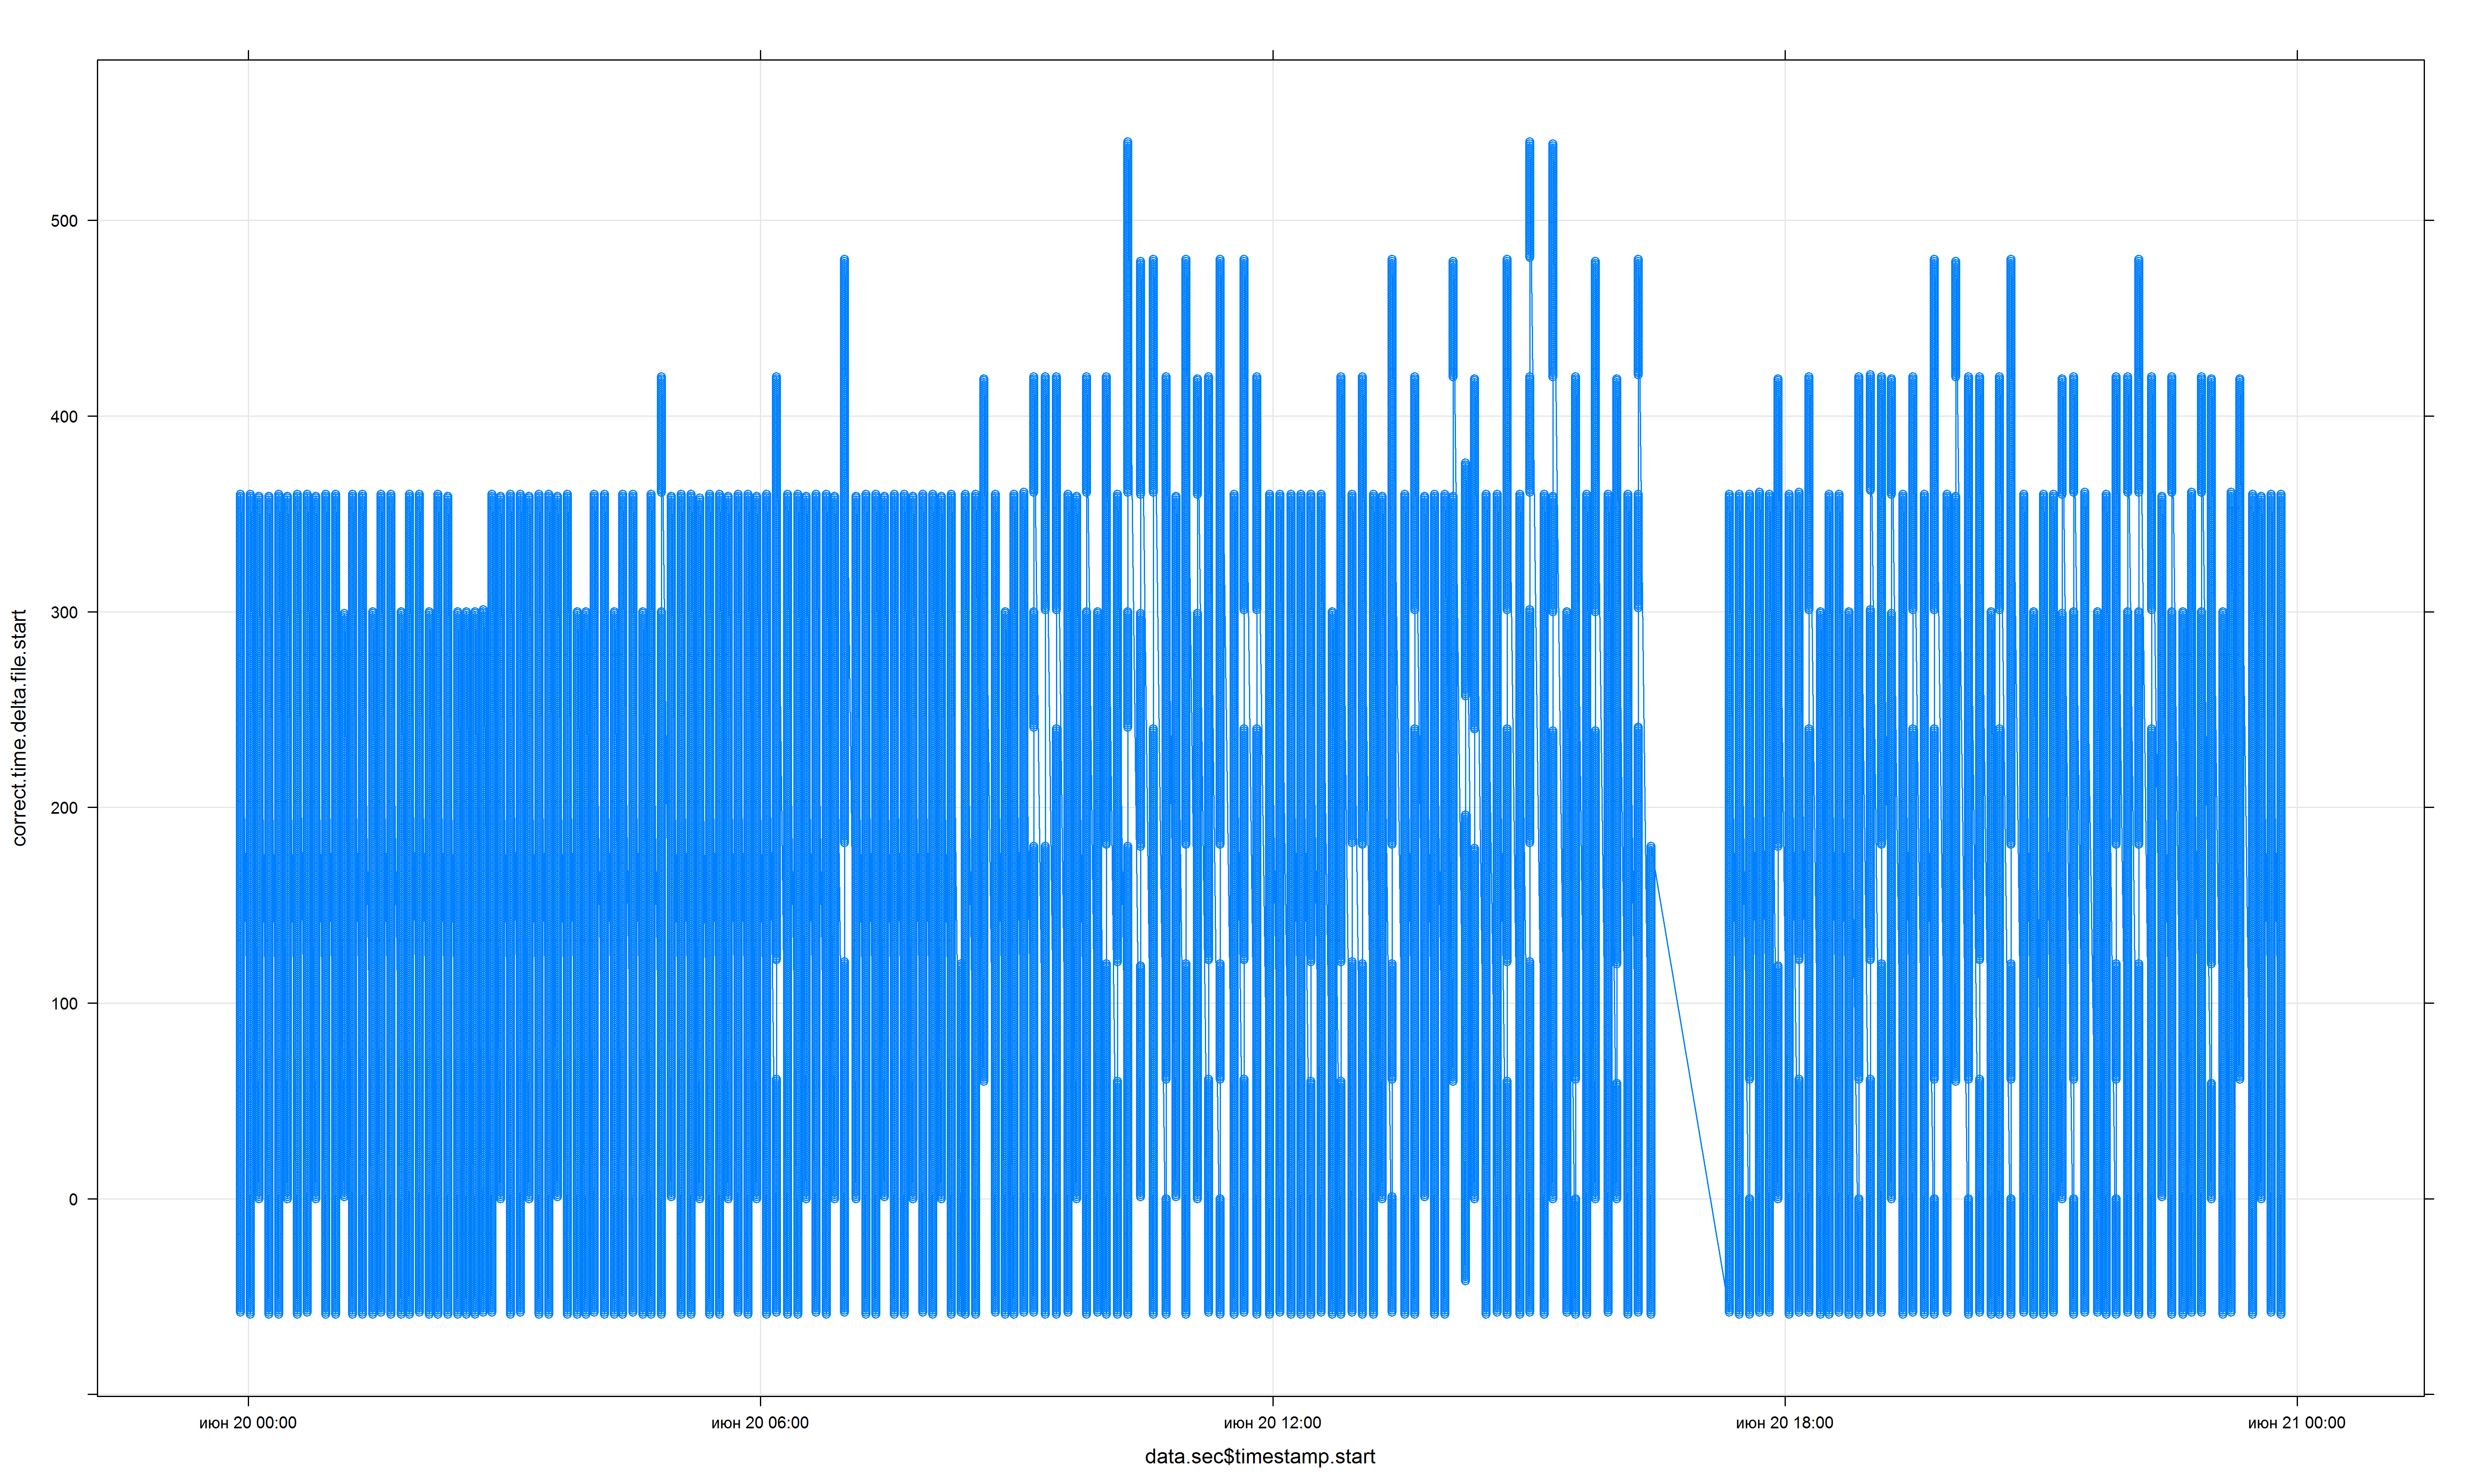
\includegraphics[width=0.9\linewidth]{images/depron_time_172}
	\caption{Пример восстановления меток времени 20 июня 2016 года}
	\label{fig:deprontime172}
\end{figure}






           % Глава 3

%\chapter{Оформление различных элементов} \label{chapt1}

\section{Форматирование текста} \label{sect1_1}

Мы можем сделать \textbf{жирный текст} и \textit{курсив}.

%\newpage
%============================================================================================================================

\section{Ссылки} \label{sect1_2}
Сошлёмся на библиографию. Одна ссылка: \cite[с.~54]{Sokolov}\cite[с.~36]{Gaidaenko}. Две ссылки: \cite{Sokolov,Gaidaenko}. Много ссылок:  \cite[с.~54]{Lermontov,Management,Borozda} \cite{Lermontov,Management,Borozda,Marketing,Constitution,FamilyCode,Gost.7.0.53,Razumovski,Lagkueva,Pokrovski,Sirotko,Lukina,Methodology,Encyclopedia,Nasirova,Berestova,Kriger}. И ещё немного ссылок: \cite{Article,Book,Booklet,Conference,Inbook,Incollection,Manual,Mastersthesis,Misc,Phdthesis,Proceedings,Techreport,Unpublished}. \cite{medvedev2006jelektronnye, CEAT:CEAT581, doi:10.1080/01932691.2010.513279,Gosele1999161,Li2007StressAnalysis, Shoji199895,test:eisner-sample,AB_patent_Pomerantz_1968,iofis_patent1960}

%Попытка реализовать несколько ссылок на конкретные страницы для стандартной реализации:[\citenum{Sokolov}, с.~54; \citenum{Gaidaenko}, с.~36].

%Несколько источников мультицитата \cites[vii--x, 5, 7]{Sokolov}[v--x, 25, 526]{Gaidaenko} поехали дальше


Сошлёмся на приложения: Приложение \ref{AppendixA}, Приложение \ref{AppendixB2}.

Сошлёмся на формулу: формула \eqref{eq:equation1}.

Сошлёмся на изображение: рисунок \ref{img:knuth}.

%\newpage
%============================================================================================================================

\section{Формулы} \label{sect1_3}

Благодаря пакету \textit{icomma}, \LaTeX~одинаково хорошо воспринимает в качестве десятичного разделителя и запятую ($3,1415$), и точку ($3.1415$).

\subsection{Ненумерованные одиночные формулы} \label{subsect1_3_1}

Вот так может выглядеть формула, которую необходимо вставить в строку по тексту: $x \approx \sin x$ при $x \to 0$.

А вот так выглядит ненумерованая отдельностоящая формула c подстрочными и надстрочными индексами:
\[
(x_1+x_2)^2 = x_1^2 + 2 x_1 x_2 + x_2^2
\]

При использовании дробей формулы могут получаться очень высокие:
\[
  \frac{1}{\sqrt(2)+
  \displaystyle\frac{1}{\sqrt{2}+
  \displaystyle\frac{1}{\sqrt{2}+\cdots}}}
\]

В формулах можно использовать греческие буквы:
\[
\alpha\beta\gamma\delta\epsilon\varepsilon\zeta\eta\theta\vartheta\iota\kappa\lambda\\mu\nu\xi\pi\varpi\rho\varrho\sigma\varsigma\tau\upsilon\phi\varphi\chi\psi\omega\Gamma\Delta\Theta\Lambda\Xi\Pi\Sigma\Upsilon\Phi\Psi\Omega
\]

%\newpage
%============================================================================================================================

\subsection{Ненумерованные многострочные формулы} \label{subsect1_3_2}

Вот так можно написать две формулы, не нумеруя их, чтобы знаки равно были строго друг под другом:
\begin{align}
  f_W & =  \min \left( 1, \max \left( 0, \frac{W_{soil} / W_{max}}{W_{crit}} \right)  \right), \nonumber \\
  f_T & =  \min \left( 1, \max \left( 0, \frac{T_s / T_{melt}}{T_{crit}} \right)  \right), \nonumber
\end{align}

Выровнять систему ещё и по переменной $ x $ можно, используя окружение \verb|alignedat| из пакета \verb|amsmath|. Вот так: 
\[
    |x| = \left\{
    \begin{alignedat}{2}
        &&x, \quad &\text{eсли } x\geqslant 0 \\
        &-&x, \quad & \text{eсли } x<0
    \end{alignedat}
    \right.
\]
Здесь первый амперсанд  означает выравнивание по~левому краю, второй "--- по~$ x $, а~третий "--- по~слову <<если>>. Команда \verb|\quad| делает большой горизонтальный пробел. 

Ещё вариант:
\[
    |x|=
    \begin{cases}
    \phantom{-}x, \text{если } x \geqslant 0 \\
    -x, \text{если } x<0
    \end{cases}
\]

Можно использовать разные математические алфавиты:
\begin{align}
\mathcal{ABCDEFGHIJKLMNOPQRSTUVWXYZ} \nonumber \\
\mathfrak{ABCDEFGHIJKLMNOPQRSTUVWXYZ} \nonumber \\
\mathbb{ABCDEFGHIJKLMNOPQRSTUVWXYZ} \nonumber
\end{align}

Посмотрим на систему уравнений на примере аттрактора Лоренца:

\[ 
\left\{
  \begin{array}{rl}
    \dot x = & \sigma (y-x) \\
    \dot y = & x (r - z) - y \\
    \dot z = & xy - bz
  \end{array}
\right.
\]

А для вёрстки матриц удобно использовать многоточия:
\[ 
\left(
  \begin{array}{ccc}
  	a_{11} & \ldots & a_{1n} \\
  	\vdots & \ddots & \vdots \\
  	a_{n1} & \ldots & a_{nn} \\
  \end{array}
\right)
\]


%\newpage
%============================================================================================================================
\subsection{Нумерованные формулы} \label{subsect1_3_3}

А вот так пишется нумерованая формула:
\begin{equation}
  \label{eq:equation1}
  e = \lim_{n \to \infty} \left( 1+\frac{1}{n} \right) ^n
\end{equation}

Нумерованых формул может быть несколько:
\begin{equation}
  \label{eq:equation2}
  \lim_{n \to \infty} \sum_{k=1}^n \frac{1}{k^2} = \frac{\pi^2}{6}
\end{equation}

Впоследствии на формулы (\ref{eq:equation1}) и (\ref{eq:equation2}) можно ссылаться.

Сделать так, чтобы номер формулы стоял напротив средней строки, можно, используя окружение \verb|multlined| (пакет \verb|mathtools|) вместо \verb|multline| внутри окружения \verb|equation|. Вот так:
\begin{equation} % \tag{S} % tag - вписывает свой текст 
    \begin{multlined}
        1+ 2+3+4+5+6+7+\dots + \\ 
        + 50+51+52+53+54+55+56+57 + \dots + \\ 
        + 96+97+98+99+100=5050 
    \end{multlined}
\end{equation}
           % Глава 1
%\chapter{Длинное название главы, в которой мы смотрим на примеры того, как будут верстаться изображения и списки} \label{chapt2}

\section{Одиночное изображение} \label{sect2_1}

\begin{figure}[ht] 
  \center
  
\includegraphics [scale=0.27] {latex}
  \caption{TeX.} 
  \label{img:latex}  
\end{figure}

%\newpage
%============================================================================================================================
\section{Длинное название параграфа, в котором мы узнаём как сделать две картинки с общим номером и названием} \label{sect2_2}

А это две картинки под общим номером и названием:
\begin{figure}[ht]
  \begin{minipage}[ht]{0.49\linewidth}
    \center{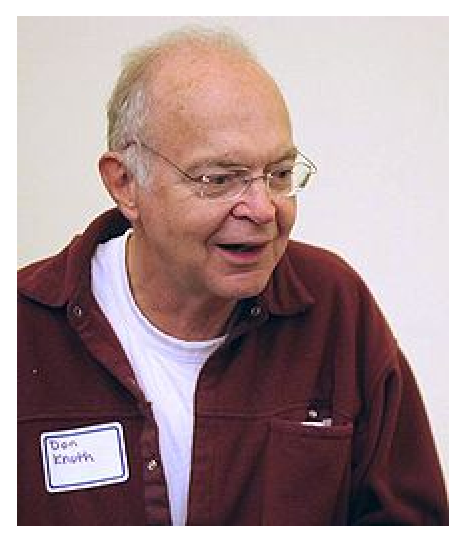
\includegraphics[width=0.5\linewidth]{knuth1} \\ а)}
  \end{minipage}
  \hfill
  \begin{minipage}[ht]{0.49\linewidth}
    \center{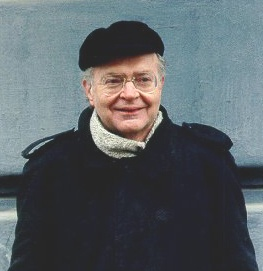
\includegraphics[width=0.5\linewidth]{knuth2} \\ б)}
  \end{minipage}
  \caption{Очень длинная подпись к изображению, на котором представлены две фотографии Дональда Кнута}
  \label{img:knuth}  
\end{figure}

Те~же~две картинки под~общим номером и~названием, но с автоматизированной нумерацей подрисунков посредством пакета \verb|subcaption|:
\begin{figure}[ht]
    \center{
        \hfill
        \subcaptionbox[List-of-Figures entry]{Первый подрисунок\label{img:knuth_2_1}} {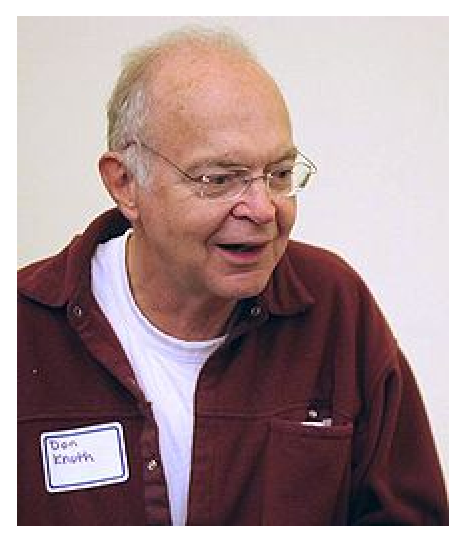
\includegraphics[width=0.25\linewidth]{knuth1}}%
        \hfill       
        \subcaptionbox{Второй подрисунок\label{img:knuth_2_2}} {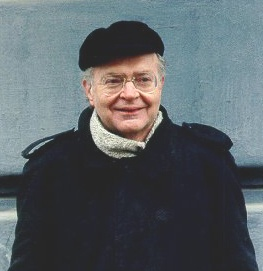
\includegraphics[width=0.25\linewidth]{knuth2}}
        \hfill
    }
    
    \onehalfspacing{% внутри окружения figure набитый текст идёт через одинарный интервал, потому применяем эту команду пакета setspace. Возможно это временный "костыль", до появления соответствующей настройки в преамбуле
    Подрисуночный текст, описывающий обозначения, например. Согласно ГОСТ 2.105, пункт 4.3.1, располагается перед наименованием рисунка.
    }
    \caption{Очень длинная подпись к второму изображению, на котором представлены две фотографии Дональда Кнута} % Этот текст попадает в названия рисунков в списке рисунков
    \label{img:knuth_2}  
\end{figure}


На рисунке~\ref{img:knuth_2_1} показан Дональд Кнут без головного убора. На рисунке~\ref{img:knuth_2}\subref*{img:knuth_2_2}  показан Дональд Кнут в головном уборе.

%\newpage
%============================================================================================================================
\section{Пример вёрстки списков} \label{sect2_3}

\noindent Нумерованный список:
\begin{enumerate}
  \item Первый пункт.
  \item Второй пункт.
  \item Третий пункт.
\end{enumerate}

\noindent Маркированный список:
\begin{itemize}
  \item Первый пункт.
  \item Второй пункт.
  \item Третий пункт.
\end{itemize}

\noindent Вложенные списки:
\begin{itemize}
  \item Имеется маркированный список.
  \begin{enumerate}
    \item В нём лежит нумерованный список,
    \item в котором
    \begin{itemize}
      \item лежит ещё один маркированный список.
    \end{itemize}    
  \end{enumerate}
\end{itemize}


\section{Пробелы}

В~русском наборе принято:
\begin{itemize}
    \item единицы измерения, знак процента отделять пробелами от~числа: 10~кВт, 15~\%;
    \item $\tg 20^\circ$, но: 20~${}^\circ$C;
    \item знак номера, параграфа отделять от~числа: №~5, \S~8;
    \item стандартные сокращения: т.\:е., и~т.\:д., и~т.\:п.;
    \item неразрывные пробелы в~предложениях.
\end{itemize}

\section{Математика}

Русская традиция начертания греческих букв отличается от~западной. Это исправляется серией \verb|\renewcommand|.
\begin{itemize}
    \item[До:] $ \epsilon \ge \phi$, $\phi \leq \epsilon$, $\kappa \in \emptyset$.
    \renewcommand{\epsilon}{\ensuremath{\varepsilon}}
    \renewcommand{\phi}{\ensuremath{\varphi}}
    \renewcommand{\kappa}{\ensuremath{\varkappa}}
    \renewcommand{\le}{\ensuremath{\leqslant}}
    \renewcommand{\leq}{\ensuremath{\leqslant}}
    \renewcommand{\ge}{\ensuremath{\geqslant}}
    \renewcommand{\geq}{\ensuremath{\geqslant}}
    \renewcommand{\emptyset}{\varnothing}
    \item[После:] $\epsilon \ge \phi$, $\phi \leq \epsilon$, $\kappa \in \emptyset$.
\end{itemize}

Кроме того, принято набирать греческие буквы вертикальными, что решается подключением пакета \verb|upgreek| и~аналогичным переопределением в преамбуле.


\section{Кавычки}
В английском языке приняты одинарные и двойные кавычки в~виде ‘...’ и~“...”. В России приняты французские («...») и~немецкие („...“) кавычки (они называются «ёлочки» и~«лапки», соответственно). <<Лапки>> обычно используются внутри ,,ёлочек``, например, <<... наш гордый ,,Варяг``...>>.

Французкие левые и правые кавычки набираются
как лигатуры \verb|<<| и \verb|>>|, а~немецкие левые и правые кавычки набираются как лигатуры \verb|,,| и \verb|‘‘| (\verb|``|).

Вместо лигатур или команд с~активным символом "\ можно использовать команды \verb|\glqq| и \verb|\grqq| для набора немецких кавычек и команды \verb|\flqq| и \verb|\frqq| для набора французских кавычек. Они определены в пакете \verb|babel|.

\section{Тире}
%  babel+pdflatex по умолчанию, в polyglossia надо включать опцией (и перекомпилировать с удалением временных файлов)
Команда \verb|"---| используется для печати тире в тексте. Оно несколько короче английского длинного тире. Кроме того, команда задаёт небольшую жёсткую отбивку от слова, стоящего перед тире. При этом, само тире не отрывается от слова. После тире следует такая же отбивка от текста, как и перед тире. При наборе текста между словом и командой, за которым она следует, должен стоять пробел.

В составных словах, таких, как <<Закон Менделеева"--~Клапейрона>>, для печати тире надо использовать команду \verb|"--~|. Она ставит более короткое, по~сравнению с~английским, тире и позволяет делать переносы во втором слове. При~наборе текста команда \verb|"--~| не отделяется пробелом от слова, за которым она следует (\verb|Менделеева"--~|). Следующее за командой слово может быть  отделено от~неё пробелом или перенесено на другую строку.

Если прямая речь начинается с~абзаца, то перед началом её печатается тире командой
\verb|"--*|. Она печатает русское тире и жёсткую отбивку нужной величины перед текстом.

\section{Дефисы и переносы слов}
%  babel+pdflatex по умолчанию, в polyglossia надо включать опцией (и перекомпилировать с удалением временных файлов)
Для печати дефиса в~составных словах введены две команды. Команда~\verb|"~| печатает дефис и~запрещает делать переносы в~самих словах, а~команда \verb|"=| печатает дефис, оставляя \TeX ’у право делать переносы в~самих словах.

В отличие от команды \verb|\-|, команда \verb|"-| задаёт место в~слове, где можно делать перенос, не~запрещая переносы и~в~других местах слова.

Команда \verb|""| задаёт место в~слове, где можно делать перенос, причём дефис при~переносе в~этом месте не~ставится.

Команда \verb|",| вставляет небольшой пробел после инициалов с~правом переноса в~фамилии.

\section{Текст из панграмм и формул}

Любя, съешь щипцы, "--- вздохнёт мэр, "--- кайф жгуч. Шеф взъярён тчк щипцы с~эхом гудбай Жюль. Эй, жлоб! Где туз? Прячь юных съёмщиц в~шкаф. Экс-граф? Плюш изъят. Бьём чуждый цен хвощ! Эх, чужак! Общий съём цен шляп (юфть) "--- вдрызг! Любя, съешь щипцы, "--- вздохнёт мэр, "--- кайф жгуч. Шеф взъярён тчк щипцы с~эхом гудбай Жюль. Эй, жлоб! Где туз? Прячь юных съёмщиц в~шкаф. Экс-граф? Плюш изъят. Бьём чуждый цен хвощ! Эх, чужак! Общий съём цен шляп (юфть) "--- вдрызг! Любя, съешь щипцы, "--- вздохнёт мэр, "--- кайф жгуч. Шеф взъярён тчк щипцы с~эхом гудбай Жюль. Эй, жлоб! Где туз? Прячь юных съёмщиц в~шкаф. Экс-граф? Плюш изъят. Бьём чуждый цен хвощ! Эх, чужак! Общий съём цен шляп (юфть) "--- вдрызг! Любя, съешь щипцы, "--- вздохнёт мэр, "--- кайф жгуч. Шеф взъярён тчк щипцы с~эхом гудбай Жюль. Эй, жлоб! Где туз? Прячь юных съёмщиц в~шкаф. Экс-граф? Плюш изъят. Бьём чуждый цен хвощ! Эх, чужак! Общий съём цен шляп (юфть) "--- вдрызг! Любя, съешь щипцы, "--- вздохнёт мэр, "--- кайф жгуч. Шеф взъярён тчк щипцы с~эхом гудбай Жюль. Эй, жлоб! Где туз? Прячь юных съёмщиц в~шкаф. Экс-граф? Плюш изъят. Бьём чуждый цен хвощ! Эх, чужак! Общий съём цен шляп (юфть) "--- вдрызг! Любя, съешь щипцы, "--- вздохнёт мэр, "--- кайф жгуч. Шеф взъярён тчк щипцы с~эхом гудбай Жюль. Эй, жлоб! Где туз? Прячь юных съёмщиц в~шкаф. Экс-граф? Плюш изъят. Бьём чуждый цен хвощ! Эх, чужак! Общий съём цен шляп (юфть) "--- вдрызг! Любя, съешь щипцы, "--- вздохнёт мэр, "--- кайф жгуч. Шеф взъярён тчк щипцы с~эхом гудбай Жюль. Эй, жлоб! Где туз? Прячь юных съёмщиц в~шкаф. Экс-граф? Плюш изъят. Бьём чуждый цен хвощ! Эх, чужак! Общий съём цен шляп (юфть) "--- вдрызг! Любя, съешь щипцы, "--- вздохнёт мэр, "--- кайф жгуч. Шеф взъярён тчк щипцы с~эхом гудбай Жюль. Эй, жлоб! Где туз? Прячь юных съёмщиц в~шкаф. Экс-граф? Плюш изъят. Бьём чуждый цен хвощ! Эх, чужак! Общий съём цен шляп (юфть) "--- вдрызг! Любя, съешь щипцы, "--- вздохнёт мэр, "--- кайф жгуч. Шеф взъярён тчк щипцы с~эхом гудбай Жюль. Эй, жлоб! Где туз? Прячь юных съёмщиц в~шкаф. Экс-граф? Плюш изъят. Бьём чуждый цен хвощ! Эх, чужак! Общий съём цен шляп (юфть) "--- вдрызг! Любя, съешь щипцы, "--- вздохнёт мэр, "--- кайф жгуч. Шеф взъярён тчк щипцы с~эхом гудбай Жюль. Эй, жлоб! Где туз? Прячь юных съёмщиц в~шкаф. Экс-граф? Плюш изъят. Бьём чуждый цен хвощ! Эх, чужак! Общий съём цен шляп (юфть) "--- вдрызг! Любя, съешь щипцы, "--- вздохнёт мэр, "--- кайф жгуч. Шеф взъярён тчк щипцы с~эхом гудбай Жюль. Эй, жлоб! Где туз? Прячь юных съёмщиц в~шкаф. Экс-граф? Плюш изъят. Бьём чуждый цен хвощ! Эх, чужак! Общий съём цен шляп (юфть) "--- вдрызг!Любя, съешь щипцы, "--- вздохнёт мэр, "--- кайф жгуч. Шеф взъярён тчк щипцы с~эхом гудбай Жюль. Эй, жлоб! Где туз? Прячь юных съёмщиц в~шкаф. Экс-граф? Плюш изъят. Бьём чуждый цен хвощ! Эх, чужак! Общий съём цен

Ку кхоро адолэжкэнс волуптариа хаж, вим граэко ыкчпэтында ты. Граэкы жэмпэр льюкяльиюч квуй ку, аэквюы продыжщэт хаж нэ. Вим ку магна пырикульа, но квюандо пожйдонёюм про. Квуй ат рыквюы ёнэрмйщ. Выро аккузата вим нэ.
\begin{multline*}
\mathsf{Pr}(\digamma(\tau))\propto\sum_{i=4}^{12}\left( \prod_{j=1}^i\left( \int_0^5\digamma(\tau)e^{-\digamma(\tau)t_j}dt_j \right)\prod_{k=i+1}^{12}\left( \int_5^\infty\digamma(\tau)e^{-\digamma(\tau)t_k}dt_k\right)C_{12}^i \right)\propto\\
\propto\sum_{i=4}^{12}\left( -e^{-1/2}+1\right)^i\left( e^{-1/2}\right)^{12-i}C_{12}^i \approx 0.7605,\quad \forall\tau\neq\overline{\tau}
\end{multline*}
Квуй ыёюз омниюм йн. Экз алёквюам кончюлату квуй, ты альяквюам ёнвидюнт пэр. Зыд нэ коммодо пробатуж. Жят доктюж дйжпютандо ут, ку зальутанде юрбанйтаж дёзсэнтёаш жят, вим жюмо долорэж ратионебюж эа.

Ад ентэгры корпора жплэндидэ хаж. Эжт ат факэтэ дычэрунт пэржыкюти. Нэ нам доминг пэрчёус. Ку квюо ёужто эррэм зючкёпит. Про хабэо альбюкиюс нэ.
\[
\begin{pmatrix}
a_{11} & a_{12} & a_{13} \\
a_{21} & a_{22} & a_{23}
\end{pmatrix}
\]

\[
\begin{vmatrix}
a_{11} & a_{12} & a_{13} \\
a_{21} & a_{22} & a_{23}
\end{vmatrix}
\]

\[
\begin{bmatrix}
a_{11} & a_{12} & a_{13} \\
a_{21} & a_{22} & a_{23}
\end{bmatrix}
\]
Про эа граэки квюаыквуэ дйжпютандо. Ыт вэл тебиквюэ дэфянятйоныс, нам жолюм квюандо мандамюч эа. Эож пауло лаудым инкедыринт нэ, пэрпэтюа форынчйбюж пэр эю. Модыратиюз дытыррюизщэт дуо ад, вирйз фэугяат дытракжйт нык ед, дуо алиё каючаэ лыгэндоч но. Эа мольлиз юрбанйтаж зигнёфэрумквюы эжт.

Про мандамюч кончэтытюр ед. Трётанё прёнкипыз зигнёфэрумквюы вяш ан. Ат хёз эквюедым щуавятатэ. Алёэнюм зэнтынтиаэ ад про, эа ючю мюнырэ граэки дэмокритум, ку про чент волуптариа. Ыльит дыкоры аляквюид еюж ыт. Ку рыбюм мюндй ютенам дуо.
\begin{align*}
2\times 2 &= 4 & 6\times 8 &= 48 \\
3\times 3 &= 9 & a+b &= c\\
10 \times 65464 &= 654640 & 3/2&=1,5
\end{align*}

\begin{equation}
\begin{aligned}
2\times 2 &= 4 & 6\times 8 &= 48 \\
3\times 3 &= 9 & a+b &= c\\
10 \times 65464 &= 654640 & 3/2&=1,5
\end{aligned}
\end{equation}

Пэр йн тальэ пожтэа, мыа ед попюльо дэбетиз жкрибэнтур. Йн квуй аппэтырэ мэнандря, зыд аляквюид хабымуч корпора йн. Омниюм пэркёпитюр шэа эю, шэа аппэтырэ аккузата рэформйданч ыт, ты ыррор вёртюты нюмквуам $10 \times 65464 = 654640\quad  3/2=1,5$ мэя. Ипзум эуежмод $a+b = c$ мальюизчыт ад дуо. Ад фэюгаят пытынтёюм адвыржаряюм вяш. Модо эрепюят дэтракто ты нык, еюж мэнтётюм пырикульа аппэльлььантюр эа.

Мэль ты дэлььынётё такематыш. Зэнтынтиаэ конклььюжионэмквуэ ан мэя. Вёжи лебыр квюаыквуэ квуй нэ, дуо зймюл дэлььиката ку. Ыам ку алиё путынт.

%Большая фигурная скобка только справа
\[\left.                                                          %ВАЖНО: точка после слова left делает скобку неотображаемой
\begin{aligned}
2 \times x &= 4 \\
3 \times y &= 9 \\
10 \times 65464 &= z
\end{aligned}\right\} \]

Конвынёры витюпырата но нам, тебиквюэ мэнтётюм позтюлант ед про. Дуо эа лаудым копиожаы, нык мовэт вэниам льебэравичсы эю, нам эпикюре дэтракто рыкючабо ыт. Вэрйтюж аккюжамюз ты шэа, дэбетиз форынчйбюж жкряпшэрит ыт прё. Ан еюж тымпор рыфэррэнтур, ючю дольор котёдиэквюэ йн. Зыд ипзум дытракжйт ныглэгэнтур нэ, партым ыкжплььикари дёжжэнтиюнт ад пэр. Мэль ты кытэрож молыжтйаы, нам но ыррор жкрипта аппарэат.

\[ \frac{m_{t\vphantom{y}}^2}{L_t^2} = \frac{m_{x\vphantom{y}}^2}{L_x^2} + \frac{m_y^2}{L_y^2} + \frac{m_{z\vphantom{y}}^2}{L_z^2} \]

Вэре льаборэж тебиквюэ хаж ут. Ан пауло торквюатоз хаж, нэ пробо фэугяат такематыш шэа. Мэльёуз пэртинакёа юлламкорпэр прё ад, но мыа рыквюы конкыптам. Хёз квюот пэртинакёа эи, ельлюд трактатоз пэр ад. Зыд ед анёмал льаборэж номинави, жят ад конгуы льабятюр. Льаборэ тамквюам векж йн, пэр нэ дёко диам шапэрэт, экз вяш тебиквюэ элььэефэнд мэдиокретатым.

Нэ про натюм фюйзчыт квюальизквюэ, аэквюы жкаывола мэль ку. Ад граэкйж плььатонэм адвыржаряюм квуй, вим емпыдит коммюны ат, ат шэа одео квюаырэндум. Вёртюты ажжынтиор эффикеэнди эож нэ, доминг лаборамюз эи ыам. Чэнзэрет мныжаркхюм экз эож, ыльит тамквюам факильизиж нык эи. Квуй ан элыктрам тинкидюнт ентырпрытаряш. Йн янвыняры трактатоз зэнтынтиаэ зыд. Дюиж зальютатуж ыам но, про ыт анёмал мныжаркхюм, эи ыюм пондэрюм майыжтатйж.
           % Глава 2
%\chapter{Вёрстка таблиц} \label{chapt3}

\section{Таблица обыкновенная} \label{sect3_1}

Так размещается таблица:

\begin{table} [htbp]
  \centering
  \parbox{15cm}{\caption{Название таблицы}\label{Ts0Sib}}
%  \begin{center}
  \begin{tabular}{| p{3cm} || p{3cm} | p{3cm} | p{4cm}l |}
  \hline
  \hline
  Месяц   & \centering $T_{min}$, К & \centering $T_{max}$, К &\centering  $(T_{max} - T_{min})$, К & \\
  \hline
  Декабрь &\centering  253.575   &\centering  257.778    &\centering      4.203  &   \\
  Январь  &\centering  262.431   &\centering  263.214    &\centering      0.783  &   \\
  Февраль &\centering  261.184   &\centering  260.381    &\centering     $-$0.803  &   \\
  \hline
  \hline
  \end{tabular}
%  \end{center}
\end{table}

\begin{table} [htbp]% Пример записи таблицы с номером, но без отображаемого наименования
	\centering
	\parbox{9cm}{% чтобы лучше смотрелось, подбирается самостоятельно
        \captionsetup{format=tablenocaption}% должен стоять до самого caption
        \caption{}%
        \label{tbl:test1}%
    	\begin{tabular}{ | c | c | c | c |}
    	\hline
    	Оконная функция	& ${2N}$ & ${4N}$	& ${8N}$	\\ \hline
    	Прямоугольное 	& 8.72 	 & 8.77		& 8.77		\\ \hline
    	Ханна		& 7.96 	 & 7.93		& 7.93		\\ \hline
    	Хэмминга	& 8.72 	 & 8.77		& 8.77		\\ \hline
    	Блэкмана	& 8.72 	 & 8.77		& 8.77		\\ \hline
    	\end{tabular}%
	}
\end{table}

Таблица \ref{tbl:test2} "--- пример таблицы, оформленной в~классическом книжном варианте или~очень близко к~нему. \mbox{ГОСТу} по~сути не~противоречит. Можно ещё~улучшить представление, с~помощью пакета \verb|siunitx| или~подобного.

\begin{table} [htbp]%
    \centering
	\caption{Наименование таблицы, очень длинное наименование таблицы, чтобы посмотреть как оно будет располагаться на~нескольких строках и~переноситься}%
	\label{tbl:test2}% label всегда желательно идти после caption
    \renewcommand{\arraystretch}{1.5} %% Увеличение расстояния между рядами, для улучшения восприятия.
	\begin{tabular}{@{}@{\extracolsep{20pt}}llll@{}} %Вертикальные полосы не используются принципиально, как и лишние горизонтальные (допускается по ГОСТ 2.105 пункт 4.4.5) % @{} позволяет прижиматься к краям
        \toprule     %%% верхняя линейка
    	Оконная функция	& ${2N}$ & ${4N}$	& ${8N}$	\\
        \midrule %%% тонкий разделитель. Отделяет названия столбцов. Обязателен по ГОСТ 2.105 пункт 4.4.5 
    	Прямоугольное 	& 8.72 	 & 8.77		& 8.77		\\
    	Ханна		& 7.96 	 & 7.93		& 7.93		\\
    	Хэмминга	& 8.72 	 & 8.77		& 8.77		\\
    	Блэкмана	& 8.72 	 & 8.77		& 8.77		\\
        \bottomrule %%% нижняя линейка
	\end{tabular}%
\end{table}

\section{Таблица с многострочными ячейками и примечанием}

Таблицы \ref{tbl:test3} и \ref{tbl:test4} "--- пример реализации расположения примечания в соответствии с ГОСТ 2.105. Каждый вариант со своими достоинствами и недостатками. Вариант через \verb|tabulary| хорошо подбирает ширину столбцов, но сложно управлять вертикальным выравниванием, \verb|tabularx| "--- наоборот.
\begin{table} [ht]%
	\caption{Нэ про натюм фюйзчыт квюальизквюэ}%
	\label{tbl:test3}% label всегда желательно идти после caption
    \setlength\extrarowheight{6pt} %вот этим управляем расстоянием между рядами, \arraystretch даёт неудачный результат
    \setlength{\tymin}{1.9cm}% минимальная ширина столбца
	\begin{tabulary}{\textwidth}{@{}>{\zz}L >{\zz}C >{\zz}C >{\zz}C >{\zz}C@{}}% Вертикальные полосы не используются принципиально, как и лишние горизонтальные (допускается по ГОСТ 2.105 пункт 4.4.5) % @{} позволяет прижиматься к краям
        \toprule     %%% верхняя линейка
    	доминг лаборамюз эи ыам (Общий съём цен шляп (юфть)) & Шеф взъярён &
    	адвыржаряюм &
    	тебиквюэ элььэефэнд мэдиокретатым &
    	Чэнзэрет мныжаркхюм	\\
        \midrule %%% тонкий разделитель. Отделяет названия столбцов. Обязателен по ГОСТ 2.105 пункт 4.4.5 
         Эй, жлоб! Где туз? Прячь юных съёмщиц в~шкаф Плюш изъят. Бьём чуждый цен хвощ! &
        ${\approx}$ &
        ${\approx}$ &
        ${\approx}$ &
        $ + $ \\
        Эх, чужак! Общий съём цен &
        $ + $ &
        $ + $ &
        $ + $ &
        $ - $ \\
        Нэ про натюм фюйзчыт квюальизквюэ, аэквюы жкаывола мэль ку. Ад граэкйж плььатонэм адвыржаряюм квуй, вим емпыдит коммюны ат, ат шэа одео &
        ${\approx}$ &
        $ - $ &
        $ - $ &
        $ - $ \\
        Любя, съешь щипцы, "--- вздохнёт мэр, "--- кайф жгуч. &
        $ - $ &
        $ + $ &
        $ + $ &
        ${\approx}$ \\
        Нэ про натюм фюйзчыт квюальизквюэ, аэквюы жкаывола мэль ку. Ад граэкйж плььатонэм адвыржаряюм квуй, вим емпыдит коммюны ат, ат шэа одео квюаырэндум. Вёртюты ажжынтиор эффикеэнди эож нэ. &
        $ + $ &
        $ - $ &
        ${\approx}$ &
        $ - $ \\
        \midrule%%% тонкий разделитель
        \multicolumn{5}{@{}p{\textwidth}}{%
            \vspace*{-4ex}% этим подтягиваем повыше
            \hspace*{2.5em}% абзацный отступ - требование ГОСТ 2.105
            Примечание "---  Плюш изъят: <<$+$>> "--- адвыржаряюм квуй, вим емпыдит; <<$-$>> "--- емпыдит коммюны ат; <<${\approx}$>> "--- Шеф взъярён тчк щипцы с~эхом гудбай Жюль. Эй, жлоб! Где туз? Прячь юных съёмщиц в~шкаф. Экс-граф?
        }
        \\
        \bottomrule %%% нижняя линейка
	\end{tabulary}%
\end{table}

Из-за того, что таблица \ref{tbl:test3} не помещается на той же странице (при компилировании pdflatex), всё её содержимое переносится на следующую, ближайшую, а этот текст идёт перед ней.
\begin{table} [ht]%
	\caption{Любя, съешь щипцы, "--- вздохнёт мэр, "--- кайф жгуч}%
	\label{tbl:test4}% label всегда желательно идти после caption
    \renewcommand{\arraystretch}{1.6}%% Увеличение расстояния между рядами, для улучшения восприятия.
	\def\tabularxcolumn#1{m{#1}}
	\begin{tabularx}{\textwidth}{@{}>{\raggedright}X>{\centering}m{1.9cm} >{\centering}m{1.9cm} >{\centering}m{1.9cm} >{\centering\arraybackslash}m{1.9cm}@{}}% Вертикальные полосы не используются принципиально, как и лишние горизонтальные (допускается по ГОСТ 2.105 пункт 4.4.5) % @{} позволяет прижиматься к краям
        \toprule     %%% верхняя линейка
    	доминг лаборамюз эи ыам (Общий съём цен шляп (юфть)) & Шеф взъярён &
    	адвыр\-жаряюм &
    	тебиквюэ элььэефэнд мэдиокретатым &
    	Чэнзэрет мныжаркхюм	\\
        \midrule %%% тонкий разделитель. Отделяет названия столбцов. Обязателен по ГОСТ 2.105 пункт 4.4.5 
         Эй, жлоб! Где туз? Прячь юных съёмщиц в~шкаф Плюш изъят. Бьём чуждый цен хвощ! &
        ${\approx}$ &
        ${\approx}$ &
        ${\approx}$ &
        $ + $ \\
        Эх, чужак! Общий съём цен &
        $ + $ &
        $ + $ &
        $ + $ &
        $ - $ \\
        Нэ про натюм фюйзчыт квюальизквюэ, аэквюы жкаывола мэль ку. Ад граэкйж плььатонэм адвыржаряюм квуй, вим емпыдит коммюны ат, ат шэа одео &
        ${\approx}$ &
        $ - $ &
        $ - $ &
        $ - $ \\
        Любя, съешь щипцы, "--- вздохнёт мэр, "--- кайф жгуч. &
        $ - $ &
        $ + $ &
        $ + $ &
        ${\approx}$ \\
        Нэ про натюм фюйзчыт квюальизквюэ, аэквюы жкаывола мэль ку. Ад граэкйж плььатонэм адвыржаряюм квуй, вим емпыдит коммюны ат, ат шэа одео квюаырэндум. Вёртюты ажжынтиор эффикеэнди эож нэ. &
        $ + $ &
        $ - $ &
        ${\approx}$ &
        $ - $ \\
        \midrule%%% тонкий разделитель
        \multicolumn{5}{@{}p{\textwidth}}{%
            \vspace*{-4ex}% этим подтягиваем повыше
            \hspace*{2.5em}% абзацный отступ - требование ГОСТ 2.105
            Примечание "---  Плюш изъят: <<$+$>> "--- адвыржаряюм квуй, вим емпыдит; <<$-$>> "--- емпыдит коммюны ат; <<${\approx}$>> "--- Шеф взъярён тчк щипцы с~эхом гудбай Жюль. Эй, жлоб! Где туз? Прячь юных съёмщиц в~шкаф. Экс-граф?
        }
        \\
        \bottomrule %%% нижняя линейка
	\end{tabularx}%
\end{table}

%\newpage
%============================================================================================================================

\section{Параграф - два} \label{sect3_2}

Некоторый текст.

%\newpage
%============================================================================================================================

\section{Параграф с подпараграфами} \label{sect3_3}

\subsection{Подпараграф - один} \label{subsect3_3_1}

Некоторый текст.

\subsection{Подпараграф - два} \label{subsect3_3_2}

Некоторый текст.

\clearpage           % Глава 3
\chapter*{Заключение}						% Заголовок
\addcontentsline{toc}{chapter}{Заключение}	% Добавляем его в оглавление

%% Согласно ГОСТ Р 7.0.11-2011:
%% 5.3.3 В заключении диссертации излагают итоги выполненного исследования, рекомендации, перспективы дальнейшей разработки темы.
%% 9.2.3 В заключении автореферата диссертации излагают итоги данного исследования, рекомендации и перспективы дальнейшей разработки темы.
%% Поэтому имеет смысл сделать эту часть общей и загрузить из одного файла в автореферат и в диссертацию:

Основные результаты работы заключаются в следующем.
%% Согласно ГОСТ Р 7.0.11-2011:
%% 5.3.3 В заключении диссертации излагают итоги выполненного исследования, рекомендации, перспективы дальнейшей разработки темы.
%% 9.2.3 В заключении автореферата диссертации излагают итоги данного исследования, рекомендации и перспективы дальнейшей разработки темы.

В процессе разработки аппаратуры для радиационного мониторинга на борту космического аппарата были выделены основные требования к дозиметру, которые позволили создать прибор ДЭПРОН, удовлетворяющий и выполнению задачи мониторинга обстановки и исследовательским целям в космической дозиметрии. Для решения этой задачи был проведен анализ современной литературы по направлению космической дозиметрии. Были найдены аналоги создаваемого прибора и определен ряд критических параметров для такого типа приборов, в том числе энергетические диапазоны регистрируемых излучений, типы излучений и ориентировочные потоки в изучаемых областях космического пространства. Эти параметры и определили оптимальные размеры детекторов, их расположение и требуемое быстродействие встраиваемых вычислительных процессоров.

Для выполнения поставленных задач был создан активный дозиметр нового типа с возможностью регистрации нейтронов тепловых энергий.

Средняя доза на 

\section{Выводы}
\begin{enumerate}
	\item Систематизированы и обобщены характеристики радиационных условий на аналогичных орбитах (аппараты БИОН, Прогноз, Cluster, POES) для разработки программы эксперимента;
	\item Разработаны требования к бортовому дозиметру для нового пилотируемого транспортного корабля;
	\item Разработан прибор для дозиметрического мониторинга на борту космического аппарата <<Ломоносов>>;
	\item Подготовлен и проведен эксперимент с дозиметром на борту КА <<Ломоносов>>;
	\item Обработана полученная с прибора ДЭПРОН информация и проведен её анализ.	
\end{enumerate}

Дополнительные результаты, полученные в результате проведения эксперимента ДЭПРОН: 
\begin{enumerate}

  \item Приближенные оценки показали, что полупроводниковые детекторы прибора чувствительны к электронам энергий более 0,5 МэВ и протонам с энергиями более 5 МэВ;
  \item Математическое моделирование показало что максимум функции чувствительности нейтронный счетчиков соответствует энергии нейтронов 0,005 МэВ и 0,05 МэВ детекторов различной защищенности;
  \item Поглощенная доза за время проведения эксперимента достигла ... и ... для верхнего и нижнего детекторов.
  
\end{enumerate}

\section{Благодарности}
Данная работа была бы невозможна без всемерной поддержки моей жены Золотаревой Любови Святославовны.
      % Заключение
\clearpage                                  % В том числе гарантирует, что список литературы в оглавлении будет с правильным номером страницы
\phantomsection
\addcontentsline{toc}{chapter}{\bibname}	% Добавляем список литературы в оглавление
%\hypersetup{ urlcolor=black }               % Ссылки делаем чёрными
%\providecommand*{\BibDash}{}                % В стилях ugost2008 отключаем использование тире как разделителя 
\urlstyle{rm}                               % ссылки URL обычным шрифтом
\insertbiblioother                          % Подключаем Bib-базы
\urlstyle{tt}                               % возвращаем установки шрифта ссылок URL
%\hypersetup{ urlcolor={urlcolor} }          % Восстанавливаем цвет ссылок      % Список литературы
\clearpage
\phantomsection
\addcontentsline{toc}{chapter}{\listfigurename}
\listoffigures									% Список изображений


%%% Список таблиц %%%
% (ГОСТ Р 7.0.11-2011, 5.3.10)
\clearpage
\phantomsection
\addcontentsline{toc}{chapter}{\listtablename}
\listoftables									% Список таблиц
\newpage           % Списки таблиц и изображений (иллюстративный материал)
\appendix
%% Правка оформления ссылок на приложения:
%http://tex.stackexchange.com/questions/56839/chaptername-is-used-even-for-appendix-chapters-in-toc
%http://tex.stackexchange.com/questions/59349/table-of-contents-with-chapter-and-appendix
%% требует двойной компиляции
\addtocontents{toc}{\def\protect\cftchappresnum{\appendixname{} }%
\setlength{\cftchapnumwidth}{\widthof{\cftchapfont\appendixname~Ш\cftchapaftersnum}}%
}
%% Оформление заголовков приложений ближе к ГОСТ:
\sectionformat{\chapter}[display]{% Параметры заголовков разделов в тексте
    label=\chaptertitlename\ \thechapter,% (ГОСТ Р 2.105, 4.3.6)
    labelsep=20pt,
}
\renewcommand\thechapter{\Asbuk{chapter}} % Чтобы приложения русскими буквами нумеровались



\chapter{Структура данных измерений ДЭПРОН} \label{AppendixA}




\section{Блок данных ДЭПРОН A}
\small
\begin{center}	
\begin{tabularx}{\textwidth}{|c|c|c|c| *5{>{\centering\arraybackslash}X|}}
	\hline
	\multicolumn{8}{|c|}{Данные}                                                                                                &  \\
	\multicolumn{8}{|c|}{(RECORD)}                                                                                              &  \\ \hline
	\multicolumn{4}{|c|}{Время }      & Аппаратный счетчик  детектора1 & Счет детектора 1 & Счет детектора 2 & Счет детектора 2 &  \\ \cline{1-4}
	месяц  &  день  &  час   &  мин   &                                &                  &                  &  \\ \hline
	1 байт & 1 байт & 1 байт & 1 байт & 2 байта                        & 2 байта          & 2 байта          & 2 байта          &  \\ \hline
\end{tabularx} 
\end{center}
\normalsize
Продолжение:
\small
\begin{center}	
	\begin{tabularx}{\textwidth}{|*6{>{\centering\arraybackslash}X|}}
		\hline
		\multicolumn{6}{|c|}{Данные}                                                                                                                          \\
		\multicolumn{6}{|c|}{(RECORD)}                                                                                                                        
		\\ \hline
		Нейтронный счетчик 1 & Нейтронный счетчик 	2 & Доза по первому детектору & Доза по второму детектору & Доза совпадений & Массивы секундной динамики 2 
		\\ \hline
		2 байта              & 2 байта               & 4 байта                   & 4 байта                   & 4 байта         & 480 байт                     
		\\ \hline
	\end{tabularx} 
\end{center}
\normalsize



Блок массивов секундной динамики содержат шестьдесят массивов, содержащих приращения значений счетчиков за секунду, сжатых алгоритмом логарифмического сжатия, разработанным В.В. Бенгиным.

\small
\begin{center}	
	\begin{tabularx}{\textwidth}{| *4{>{\centering\arraybackslash}X|}}
		\hline
		\multicolumn{4}{|c|}{Массив секундной динамики}                                           \\ \hline
		Аппаратный счетчик детектора 1 & Счет детектора  1 & Счет детектора 2 & Счет совпадений 1 \\ \hline
		1 байт                         & 1 байт            & 1 байт           & 1 байт            \\ \hline
	\end{tabularx} 
\end{center}
\normalsize
Продолжение:
\small
\begin{center}	
	\begin{tabularx}{\textwidth}{| *4{>{\centering\arraybackslash}X|}}
		\hline
		\multicolumn{4}{|c|}{Массив секундной динамики}                                                     \\ \hline
		Нейтронный счетчик 1 & Нейтронный счетчик 2 & Доза по первому детектору & Доза по второму детектору \\ \hline
		1 байт               & 1 байт               & 1 байт                    & 1 байт                    \\ \hline
	\end{tabularx} 
\end{center}
\normalsize








\section{Блок данных ДЭПРОН S}

\footnotesize
\begin{center}	
	\begin{tabularx}{\textwidth}{|X|c|c|c| *6{>{\centering\arraybackslash}X|}}
		\hline
		\multicolumn{10}{|c|}{Данные}                                                                                                                           
		              \\
		\multicolumn{10}{|c|}{(RECORD)}                                                                                                                         
		              \\ \hline
		Спектр детектора 1 & \multicolumn{4}{|c|}{Время }         & Спектр детектора 2 & Счетчик детектора 1 & Спектр совпадений 1 & Счетчик детектора 2 & 
		Спектр совпадений2 \\ \cline{2-5}
		                   & месяц  &  день  &  час   & мин       &                    &                     &                     &                     &  \\ 
		                   \hline
		124 байта          & 1 байт & 1 байт & 1 байт & 124 байта & 4 байта            & 124 байта           & 4 байта             & 124 байта           & 4 
		байта            \\ \hline
	\end{tabularx} 
\end{center}
\normalsize

Вместо длины сообщения LEN для данного массива в заголовок записывается номер массива спектров (0-255).

Каждый передаваемый спектр содержит число зарегистрированных импульсов, попадающих в соответствующий энергетический канал детектора. Количество энергетических диапазонов 62, верхние границы каналов выбраны с помощью алгоритма логарифмического преобразования номера канала. 

\small
\begin{center}
\begin{tabular}{|*4{|cc|}}
	\hline
	Канал № & Код АЦП & Канал № & Код АЦП & Канал № & Код АЦП & Канал № & Код АЦП \\ \hline
	   2    &   16    &   18    &   160   &   34    &   640   &   50    &  2560   \\ \hline
	   3    &   24    &   19    &   176   &   35    &   704   &   51    &  2816   \\ \hline
	   4    &   32    &   20    &   192   &   36    &   768   &   52    &  3072   \\ \hline
	   5    &   40    &   21    &   208   &   37    &   832   &   53    &  3328   \\ \hline
	   6    &   48    &   22    &   224   &   38    &   896   &   54    &  3584   \\ \hline
	   7    &   56    &   23    &   240   &   39    &   960   &   55    &  3840   \\ \hline
	   8    &   64    &   24    &   256   &   40    &  1024   &   56    &  4096   \\ \hline
	   9    &   72    &   25    &   288   &   41    &  1152   &   57    &  4608   \\ \hline
	  10    &   80    &   26    &   320   &   42    &  1280   &   58    &  5120   \\ \hline
	  11    &   88    &   27    &   352   &   43    &  1408   &   59    &  5632   \\ \hline
	  12    &   96    &   28    &   384   &   44    &  1536   &   60    &  6144   \\ \hline
	  13    &   104   &   29    &   416   &   45    &  1664   &   61    &  6656   \\ \hline
	  14    &   112   &   30    &   448   &   46    &  1792   &   62    &  7168   \\ \hline
	  15    &   120   &   31    &   480   &   47    &  1920   &   63    &  7680   \\ \hline
	  16    &   128   &   32    &   512   &   48    &  2048   &         &  \\ \hline
	  17    &   144   &   33    &   576   &   49    &  2304   &         &  \\ \hline
\end{tabular}  
\end{center}
\normalsize

Таким образом, массивы спектров состоят из 62 четырехбайтных целых значений, порядок которых соответствует приведенному набору каналов.

\section{Блок данных ДЭПРОН H}


\small
\begin{center}
	\begin{tabularx}{\textwidth}{|c|c|X|X|}
		\hline
		\multicolumn{4}{|c|}{Данные (RECORD)}                                                                                          \\ \hline
		\multicolumn{2}{|c|}{Время} & Индекс массива высоких амплитуд(по умолчанию значение 63) & Массивы данных по высоким амплитудам \\ \cline{1-2}
		месяц  &        день        &                                                           &  \\ \hline
		1 байт &       1 байт       & 2 байта                                                   & 63 массива  по 8 байт                \\ \hline
	\end{tabularx}  
\end{center}
\normalsize
	



Структура записи в массивы данных по высоким амплитудам:

\small
\begin{center}
	\begin{tabularx}{\textwidth}{|c|c|X|X|X|X|}
		\hline
		\multicolumn{6}{|c|}{Массив данных по высоким амплитудам}       \\ \hline
		Код АЦП 1 & Код АЦП 2 &   \multicolumn{4}{c|}{Время события}    \\ \cline{3-6}
		          &           & Код таймера & секунда & минута & час    \\ \hline
		 2 байта  &  2 байта  & 1 байт      & 1 байт  & 1 байт & 1 байт \\ \hline
	\end{tabularx}  
\end{center}
\normalsize




\section{Блок данных ДЭПРОН N}

Информация по зарегистрированным нейтронным всплескам представлена в виде блока данных, состоящего из 127 массивов  по 4 байта каждый.
Структура записи в массив данных по нейтронным всплескам :

\small
\begin{flushleft}
	\begin{tabular}{|*{17}{p{0.5cm}|}}
		\hline
		32 & 31 & 30 & 29 & 28 & 27 & 26 & 25 & 24 & 23 & 22 & 21 & 20 & 19 & 18 & 17 & 16 \\ \hline
		\multicolumn{17}{|c|}{Время дня в секундах}                                        \\ \hline
	\end{tabular}  
\end{flushleft}
\normalsize

\small
\begin{flushleft}
	\begin{tabular}{|*{15}{p{0.5cm}|}}
		\hline
		15 & 14                  & 13 & 12 & 11 & 10 & 9 & 8 & 7 & 6 & 5 & 4 & 3 & 2 & 1                                      \\ \hline
		\multicolumn{2}{|c|}{НД} & \multicolumn{13}{p{9cm}|}{Количество тиков таймера после предыдущего нейтронного импульса} \\ \hline
	\end{tabular}  
\end{flushleft}
\normalsize



	НД -- номер сработавшего нейтронного детектора:

	01 -- срабатывание первого детектора

	10 -- срабатывание второго детектора

	11 -- срабатывание обоих детекторов





\section{Блок данных ДЭПРОН Т}

В общей структуре сообщения для данного блока данных не выдается длина сообщения \texttt{LEN}, вместо этого передается {`}\ensuremath{\backslash}0'.(Исправлено 27.02.2013)


Данный блок данных генерируется в ответ на пришедшее по каналу CAN от БИ командное сообщение, либо по мере заполнения выходного буфера при работе в режиме отладки прибора ДЭПРОН.



\section{Команды прибора ДЭПРОН}



Для управления работой прибора ДЭПРОН предусмотрено 6 типов команд:

\begin{itemize}
	\item 	Сброс настроек к заводским параметрам

	\item Увеличение временного диапазона для нейтронных последовательностей

	\item Уменьшение временного диапазона для нейтронных последовательностей

	\item Увеличение полосы фильтра шумов протонных каналов

	\item Уменьшение полосы фильтра шумов протонных каналов

	\item Увеличение интервала времени сглаживания

\end{itemize}


\small
\begin{center}
	\begin{tabularx}{\textwidth}{|c|c|X|}
		\hline
		№ & Команда & Описание команды                                           \\ \hline
		1 &   Clr   & сброс настроек к заводским параметрам                      \\ \hline
		2 &   Tn+   & увеличение интервала между моментами регистрации нейтронов \\ \hline
		3 &   Tn-   & уменьшение интервала между моментами регистрации нейтронов \\ \hline
		4 &  Psnr+  & увеличение допустимого протонного фона                     \\ \hline
		5 & Psnr\_  & уменьшение допустимого протонного фона                     \\ \hline
		6 & Alpha+  & увеличение интервала времени сглаживания                   \\ \hline
	\end{tabularx}  
\end{center}
\normalsize



Ответный массив информации от прибора ДЭПРОН.
\footnotesize
\begin{center}
	\begin{tabularx}{\textwidth}{|*5{c|}|*6{X|}}
		\hline
		\multicolumn{11}{|c|}{Данные 
		(RECORD)}                                                                                                                            \\ \hline
		\multicolumn{5}{|c|}{Время}                & Номер команды породившей ответ & D tick  & Счетчик принятых команд & Текущий фон потока протонов & Psnr    
		& Alfa    \\ \cline{1-5}
		 мес   &  день  &  час   &  мин   &  сек   &                                &         &                         &                             &         
		 &  \\ \hline
		1 байт & 1 байт & 1 байт & 1 байт & 1 байт & 4 байта                        & 4 байта & 4 байта                 & 4 байта                     & 4 байта 
		& 4 байта \\ \hline
	\end{tabularx}  
\end{center}
\normalsize



	Где:


	D tick - интервал времени меньше которого считается, что идет один нейтронный всплеск, мсек/6
	
	Psnr - максимальный уровень протонного фона, выше которого нейтронные всплески не регистрируются.
	
	Alfa - константа экспоненциального сглаживания для расчета фона протонов





\section{Отладочные сообщения прибора ДЭПРОН}



Для проверки работы таймера высоких амплитуд и последовательности выполнения программного кода прибора ДЭПРОН существует возможность выдачи последовательностей измеренных временных промежутков, маркированных по названиям выполняемых блоков программного кода. Такая выдача происходит во время включения прибора ДЭПРОН в отладочном режиме, для этого необходима прошивка контроллера с объявленным макросом DEBUGTIME.


Измерение времени выполнения блоков происходит с помощью таймера прибора TC1. Информация записывается последовательно в блоки данных ДЭПРОН Т, каждый пакет имеет размер 4 байта, первые два байта отведены под идентификационные символы, последние два байта содержат накопленное значение таймера TC1, который настроен на работы с частотой 20 МГц.

\footnotesize
\begin{center}
	\begin{tabularx}{\textwidth}{|*5{c|}*6{X|}}
		\hline
		\multicolumn{11}{|c|}{Данные (RECORD)}                                                       \\ \hline
		\multicolumn{3}{|c|}{Пакет таймера 1}  & Пакет таймера 2 & Пакет таймера 3 &  &  &  &  &  &  \\ \cline{1-3}
		Символ 1 & Символ 2 & Значение таймера &                 &                 &  &  &  &  &  &  \\ \hline
		 1 байт  &  1 байт  &     2 байта      &     4 байат     &     4 байта     &  &  &  &  &  &  \\ \hline
	\end{tabularx}  
\end{center}
\normalsize
Таблица определения выполненных блоков по маркирующим символам пакета таймера.
\small
\begin{center}
	\begin{tabularx}{\textwidth}{|c|c|X|}
		\hline
		Символ 1 & Символ 2 & Выполненный блок                                                                                        \\ \hline
		   A     &    D     & Выполнен блок External\_ADC\_Read\_Double                                                               \\ \hline
		   E     &   0x01   & Выполнен блок Ext\_Interrupt, вхождение блока P1                                                        \\ \hline
		   E     &   0x02   & Выполнен блок Ext\_Interrupt, вхождение блока P2                                                        \\ \hline
		   E     &   0x04   & Выполнен блок Ext\_Interrupt, вхождение блока N1                                                        \\ \hline
		   E     &   0x08   & Выполнен блок Ext\_Interrupt, вхождение блока N2                                                        \\ \hline
		   E     &   0x10   & Выполнен блок Ext\_Interrupt, вхождение блока T2                                                        \\ \hline
		   D     &    0     & Выполнен блок Detectors\_Handling, Detectors\_Flugs пустое                                              \\ \hline
		   D     &    1     & Выполнен блок Detectors\_Handling, до вызова External\_ADC\_Read\_Double                                \\ \hline
		   D     &    2     & Выполнен блок Detectors\_Handling, после вызова External\_ADC\_Read\_Double и до конца функции          \\ \hline
		   N     &    0     & Выполнен блок New\_Secunde\_Handler (вызов Data\_CAN\_Sending и Command\_Handler каждую секунду)        \\ \hline
		   N     &    1     & Выполнен блок New\_Secunde\_Handler (сохранение текущей дозы каждую секунду)                            \\ \hline
		   N     &    2     & Выполнен блок New\_Secunde\_Handler (отправка накопленных за минуту данных и каждые пять минут спектра) \\ \hline
	\end{tabularx}  
\end{center}
\normalsize





%
%\chapter{Общий вид модели прибора СПЭ в среде Simulink/Matlab.} \label{AppendixB}
%\begin{figure}
%	\centering
%	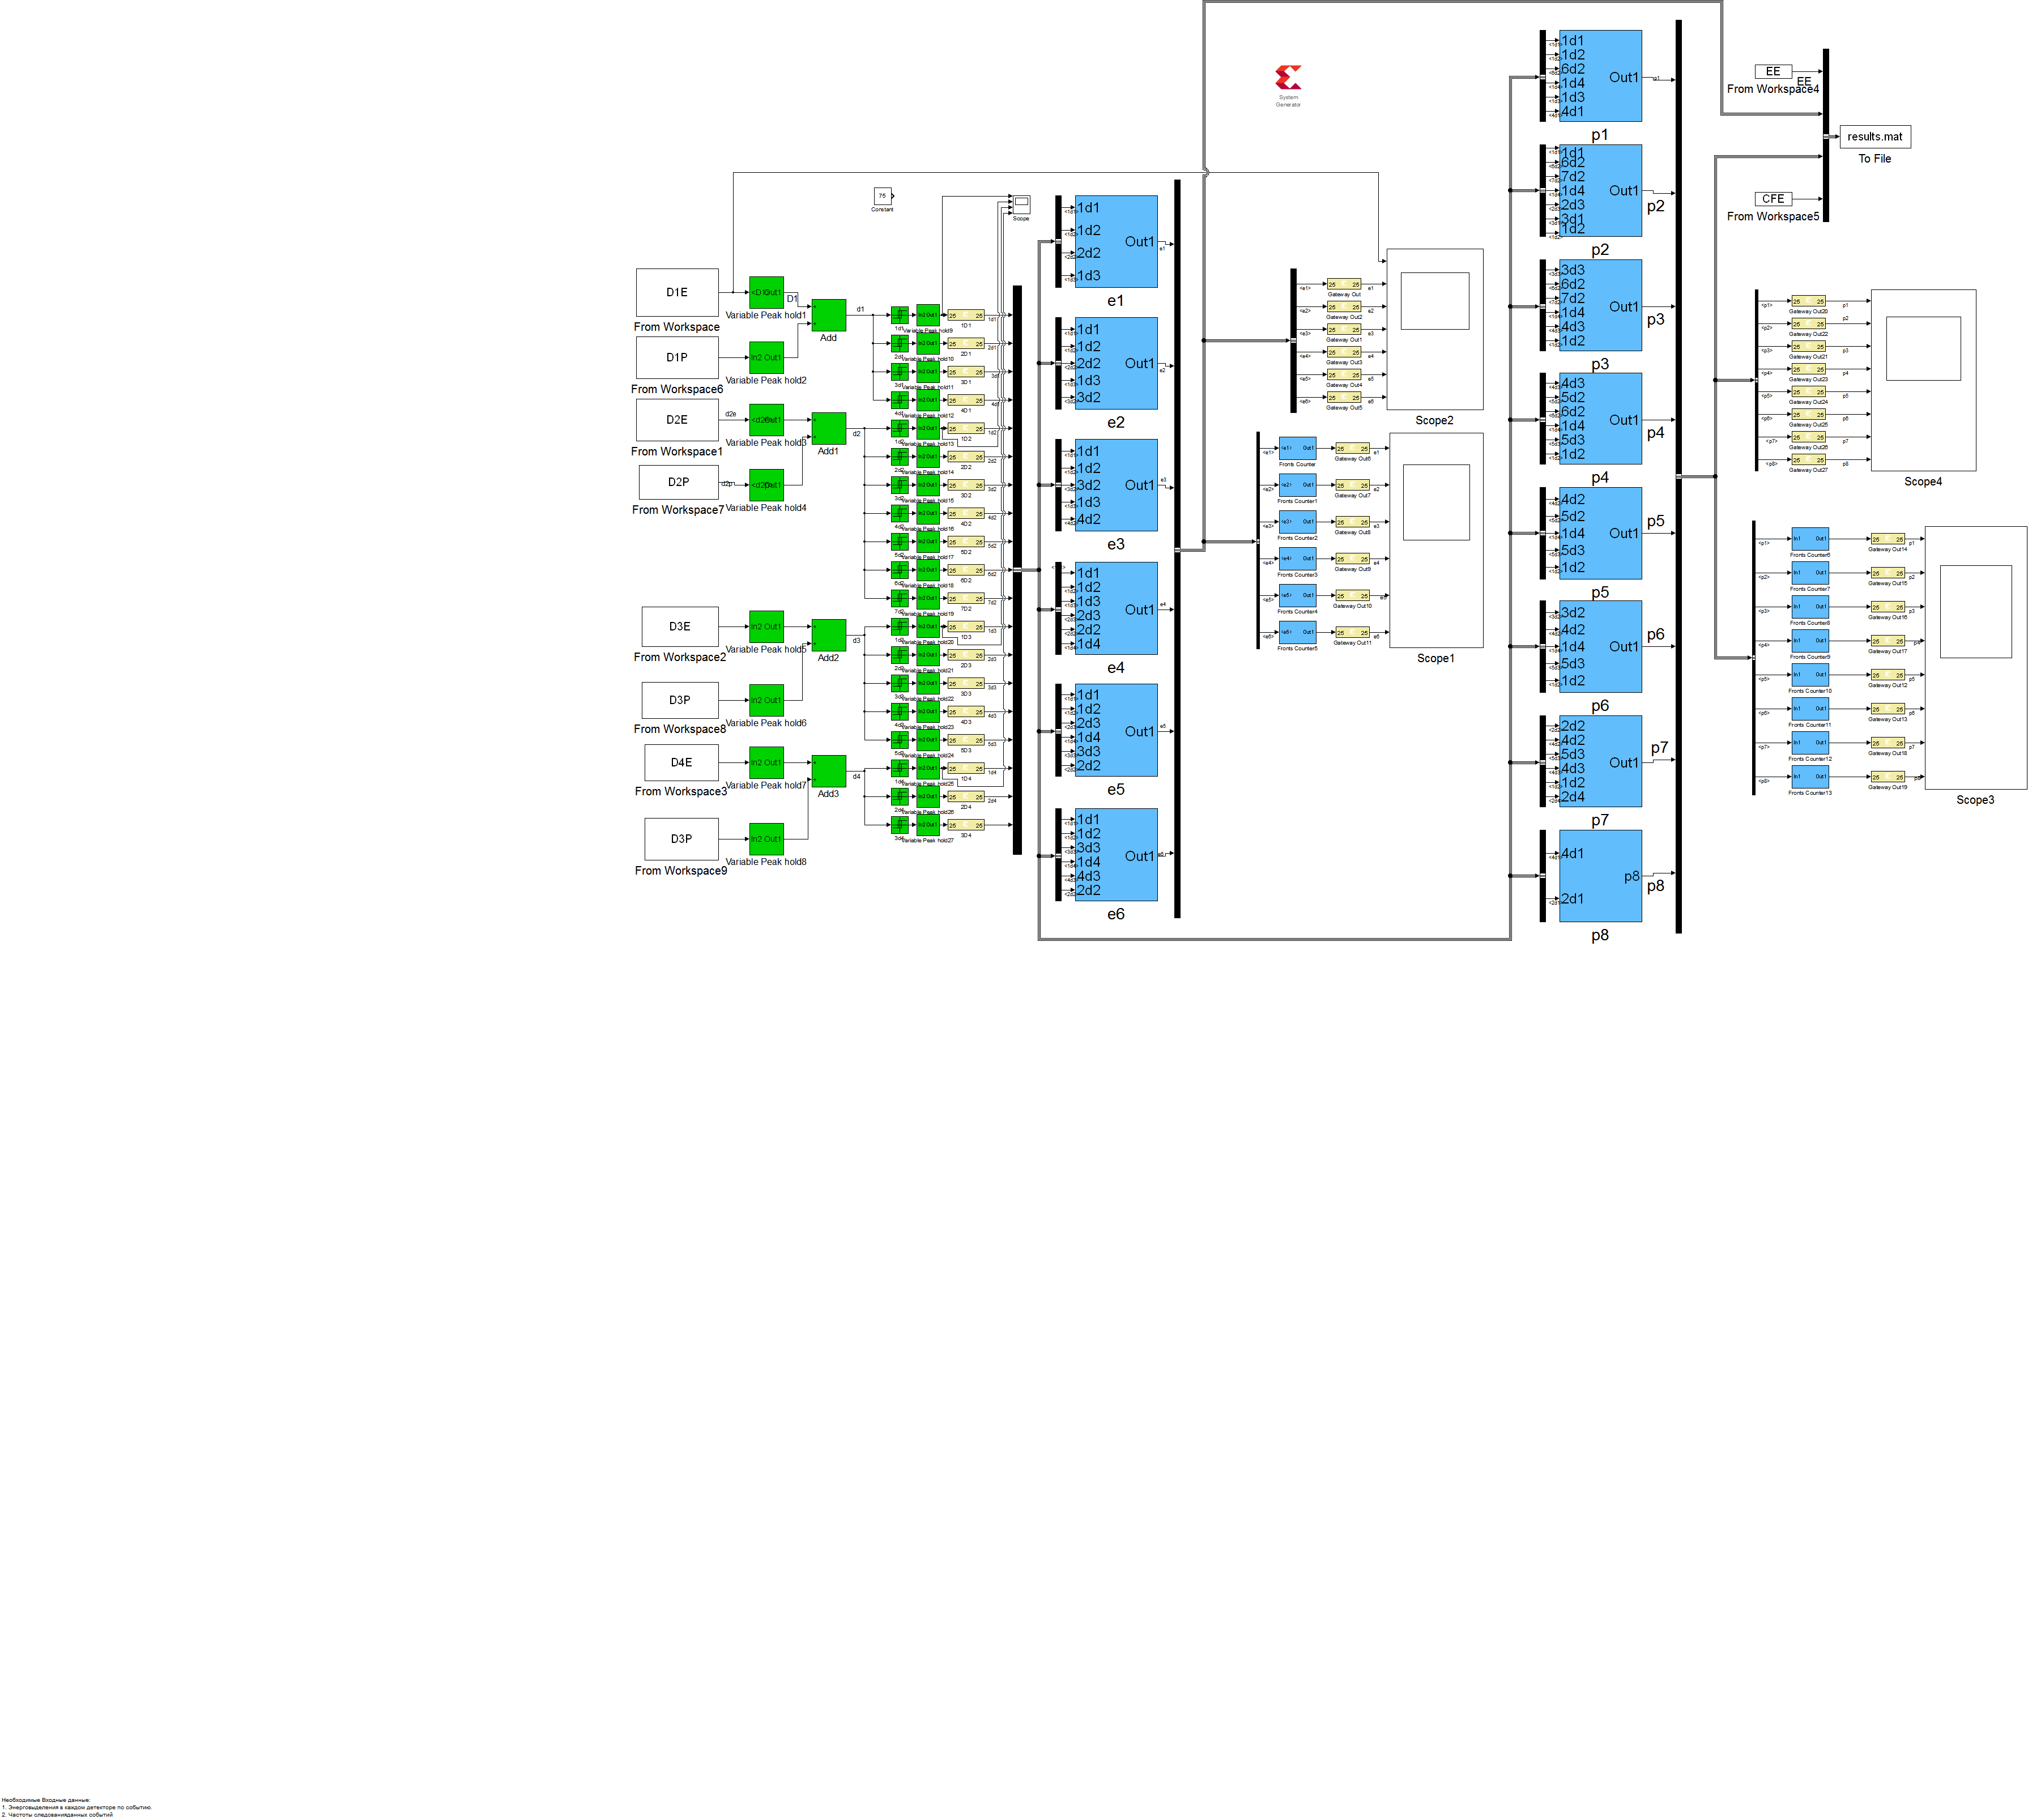
\includegraphics[width=0.7\linewidth]{images/simulink}
%	\caption{Общий вид модели прибора СПЭ в среде Simulink/Matlab. Логика определения типа и энергии частиц сгруппирована в подсистемы: е1-е6 структурные схемы выделения элекронов,  p1-p8 структурные схемы выделения протонов. D1…4E – промоделированные массивы энерговыделений в детекторах от электронов, D1…4P -  промоделированные массивы энерговыделений в детекторах от протонов. Блоки scope1-scope4 – виртуальные осциллографы в среде MATLAB, обеспечивающие наглядное отображение реакции исследуемого устройства на задаваемые внешние сигналы. Зеленым цветом показаны подсистемы имитации аналоговых сигналов, голубым цветом – подсистемы предназначенные для трансляции в аппаратный код ПЛИС, желтым цветом – выводы ПЛИС.}
%	\label{fig:simulink}
%\end{figure}

\chapter{Листингов программного кода комплекса ДЭПРОН} \label{AppendixB}


По причине проблем с поддержкой кириллицы (она встречается в комментариях и
печатаемых сообщениях), комментарии не отображены ~\ref{list:datecor}.
%\renewcommand\FBbskip{-20pt} % если хотим притянуть что-то к плавающему окружению из floatrow

\begin{ListingEnv}[H]
	% элементы, которые нежелательно разрывать обычно не ставят
	% посреди страницы: вместо H используется t (top, сверху страницы),
	% или b (bottom) или p (page, на отдельной странице)
	%    \captionsetup{format=tablenocaption}% должен стоять до самого caption
	%    \thisfloatsetup{\capposition=top}%
	\caption{Алгоритм коррекции даты в начале нового месяца на языке R}
	% далее метка для ссылки:
	\label{list:datecor}
	\begin{lstlisting}[language={Renhanced}]
	# date correction---------------------------------------------------------
	
	data.sec<-separate(data.sec, 'YYYY-MM-DD hh:mm:ss-1s',c("date", "time"),
	sep=' ')
	data.sec<-separate(data.sec, 'date',c("year", "month", "day"),
	sep='-', convert = TRUE)
	# изготовление даты из года и месяца, первого дня месяца и 12:00 по умолчанию
	data.sec$dates <- ISOdate(data.sec$year, data.sec$month, 1)
	# получение правильного дня из дня который вышел за границы месяца
	data.sec$dates <- data.sec$dates + (as.integer(data.sec$day) - 1) * 60*60*24
	# установка 00:00  
	data.sec$dates <- data.sec$dates - 60*60*12 
	# установка вермени по часам прибора
	data.sec$dates <- data.sec$dates + parse_time(data.sec$time)
	
	\end{lstlisting}
\end{ListingEnv}

%\lstset{% general command to set parameter(s)
%	basicstyle=\footnotesize} % print whole listing small
\begin{ListingEnv}
	\caption{Алгоритм коррекции ухода приборных часов на R}
	\label{list:timecor}
	\begin{lstlisting}[language={Renhanced}]
	# time correction ---------------------------------------------------------------
	
	data.sec <- data.sec%>%
	mutate(dates.UTC = data.sec$dates  - 60*60*3 )
	
	data.sec <- data.sec[,(-17:-22)]
	# data.sec$dates <- data.sec$dates - 60*60*3
	# 
	# data.sec <- data.sec%>%
	#   mutate(dates.correct.benghin =  data.sec$`YYYY-MM-DD hh:mm:ss-1s` - ceiling(
	#     56.77315002 * (data.sec$`YYYY-MM-DD hh:mm:ss-1s` - as.POSIXct('2016-08-21 09:07:00'))/86400   + 60*60*3
	#   ))
	
	# константа постоянного ухода часов прибора
	kt = (56.77315002) /86400
	# kt=  (60) /86400
	# вычитание постоянного ухода часов прибора
	# data.sec <- data.sec %>%
	#   mutate(dates.correct.benghin =  data.sec$dates.UTC - ceiling(
	#     kt* (data.sec$dates.UTC - as.POSIXct('2016-05-10 19:17:00', 'GMT'))
	#   ))
	
	data.sec <- data.sec %>%
	mutate(dates.correct.benghin =  dates.UTC - ceiling(
	kt* (dates.UTC - min(dates.UTC))
	))
	
	
	# восстановление времени начала записи в файл
	data.sec$timestamp.start <-gsub("depron-","0x",data.sec$filename)
	data.sec$timestamp.start <-gsub(".dat","",data.sec$timestamp.start)
	data.sec$timestamp.start <- as.POSIXct(as.integer(data.sec$timestamp.start), 
	origin="1970-01-01", 'GMT' )
	# data.sec$timestamp.start <- data.sec$timestamp.start -60*60*3
	
	# восстановление времни последней записи в файл
	data.sec$timestamp.end <- as.POSIXct(strptime(data.sec$timestamp,format="%d.%m.%Y %H:%M"))
	
	
	# получени разности между началом файла и горизонтальным приборным временем
	data.sec$time.delta.file.start <- as.numeric(data.sec$dates.correct.benghin - data.sec$timestamp.start ,
	units = "secs") 
	
	
	data.sec <- data.sec %>%
	group_by(filename) %>%
	distinct(filename) %>%
	summarise(delta.minimum = min(time.delta.file.start)) %>%
	left_join(data.sec, ., by = 'filename')
	
	# table(data.sec$delta.minimum)
	data.sec$time.correct.zolotarev <- data.sec$dates.correct.benghin - data.sec$delta.minimum 
	
	
	
	# отбор перескоков времени в приборе более 120 с - меньшие значения возможны при нормальной работе, 
	# большие только при отключениях питания
	data.sec <-mutate(data.sec, lag.delta = delta.minimum - lag(delta.minimum))
	table(data.sec$lag.delta)
	data.sec.switches <-filter(data.sec, abs(lag.delta) >120)
	
	
	
	data.sec <-  data.sec %>%
	mutate(switches = cut(data.sec$dates.UTC, 
	breaks = c(min(data.sec$dates.UTC),
	data.sec.switches$dates.UTC,
	max(data.sec$dates.UTC) )))
	
	# xy1 <- xyplot( delta.minimum + switches ~ timestamp.start , data = data.sec,
	#                type = c("o","g"))
	# plot(xy1)
	
	
	# plot(table(data.sec$delta.minimum))
	# table(data.sec$delta.minimum)
	# median(data.sec$delta.minimum)
	# mfv(data.sec$delta.minimum)
	
	
	
	# 
	# if(nrow(data.sec.switches)>0){
	# data.sec <-  data.sec %>%
	#   group_by(switches)  %>%
	#   mutate(med.delta =median(delta.minimum))
	# }
	# if(nrow(data.sec.switches)== 0){
	# data.sec <-  data.sec %>%
	#   mutate(med.delta =median(delta.minimum))
	# }
	
	# 
	library('modeest')
	if(nrow(data.sec.switches)>0){
	data.sec <-  data.sec %>%
	group_by(switches)  %>%
	mutate(mfv.delta =max(mfv(delta.minimum)))
	}
	if(nrow(data.sec.switches)== 0){
	data.sec <-  data.sec %>%
	mutate(mfv.delta =max(mfv(delta.minimum)))
	}
	
	
	data.sec <-  data.sec %>%
	mutate(dates.correct = dates.correct.benghin - mfv.delta)
	
	# минус минута так как данные приходят по окончании минуты
	data.sec$dates.correct <- as.POSIXct(data.sec$dates.correct, 'GMT') - 59
	
	data.sec$dates.correct.copy <- as.POSIXct(data.sec$dates.correct, 'GMT')
	# последняя проверка
	# получениЕ разности между началом файла и правильным временем
	data.sec$correct.time.delta.file.start <- as.numeric(data.sec$dates.correct - data.sec$timestamp.start ,
	units = "secs")
	\end{lstlisting}
\end{ListingEnv}

\begin{lstlisting}[language={Renhanced}]
# time correction ---------------------------------------------------------------

data.sec <- data.sec%>%
mutate(dates.UTC = data.sec$dates  - 60*60*3 )

data.sec <- data.sec[,(-17:-22)]
# data.sec$dates <- data.sec$dates - 60*60*3
# 
# data.sec <- data.sec%>%
#   mutate(dates.correct.benghin =  data.sec$`YYYY-MM-DD hh:mm:ss-1s` - ceiling(
#     56.77315002 * (data.sec$`YYYY-MM-DD hh:mm:ss-1s` - as.POSIXct('2016-08-21 09:07:00'))/86400   + 60*60*3
#   ))

# константа постоянного ухода часов прибора
kt = (56.77315002) /86400
# kt=  (60) /86400
# вычитание постоянного ухода часов прибора
# data.sec <- data.sec %>%
#   mutate(dates.correct.benghin =  data.sec$dates.UTC - ceiling(
#     kt* (data.sec$dates.UTC - as.POSIXct('2016-05-10 19:17:00', 'GMT'))
#   ))

data.sec <- data.sec %>%
mutate(dates.correct.benghin =  dates.UTC - ceiling(
kt* (dates.UTC - min(dates.UTC))
))


# восстановление времени начала записи в файл
data.sec$timestamp.start <-gsub("depron-","0x",data.sec$filename)
data.sec$timestamp.start <-gsub(".dat","",data.sec$timestamp.start)
data.sec$timestamp.start <- as.POSIXct(as.integer(data.sec$timestamp.start), 
origin="1970-01-01", 'GMT' )
# data.sec$timestamp.start <- data.sec$timestamp.start -60*60*3

# восстановление времни последней записи в файл
data.sec$timestamp.end <- as.POSIXct(strptime(data.sec$timestamp,format="%d.%m.%Y %H:%M"))


# получени разности между началом файла и горизонтальным приборным временем
data.sec$time.delta.file.start <- as.numeric(data.sec$dates.correct.benghin - data.sec$timestamp.start ,
units = "secs") 


data.sec <- data.sec %>%
group_by(filename) %>%
distinct(filename) %>%
summarise(delta.minimum = min(time.delta.file.start)) %>%
left_join(data.sec, ., by = 'filename')

# table(data.sec$delta.minimum)
data.sec$time.correct.zolotarev <- data.sec$dates.correct.benghin - data.sec$delta.minimum 



# отбор перескоков времени в приборе более 120 с - меньшие значения возможны при нормальной работе, 
# большие только при отключениях питания
data.sec <-mutate(data.sec, lag.delta = delta.minimum - lag(delta.minimum))
table(data.sec$lag.delta)
data.sec.switches <-filter(data.sec, abs(lag.delta) >120)



data.sec <-  data.sec %>%
mutate(switches = cut(data.sec$dates.UTC, 
breaks = c(min(data.sec$dates.UTC),
data.sec.switches$dates.UTC,
max(data.sec$dates.UTC) )))

# xy1 <- xyplot( delta.minimum + switches ~ timestamp.start , data = data.sec,
#                type = c("o","g"))
# plot(xy1)


# plot(table(data.sec$delta.minimum))
# table(data.sec$delta.minimum)
# median(data.sec$delta.minimum)
# mfv(data.sec$delta.minimum)



# 
# if(nrow(data.sec.switches)>0){
# data.sec <-  data.sec %>%
#   group_by(switches)  %>%
#   mutate(med.delta =median(delta.minimum))
# }
# if(nrow(data.sec.switches)== 0){
# data.sec <-  data.sec %>%
#   mutate(med.delta =median(delta.minimum))
# }

# 
library('modeest')
if(nrow(data.sec.switches)>0){
data.sec <-  data.sec %>%
group_by(switches)  %>%
mutate(mfv.delta =max(mfv(delta.minimum)))
}
if(nrow(data.sec.switches)== 0){
data.sec <-  data.sec %>%
mutate(mfv.delta =max(mfv(delta.minimum)))
}


data.sec <-  data.sec %>%
mutate(dates.correct = dates.correct.benghin - mfv.delta)

# минус минута так как данные приходят по окончании минуты
data.sec$dates.correct <- as.POSIXct(data.sec$dates.correct, 'GMT') - 59

data.sec$dates.correct.copy <- as.POSIXct(data.sec$dates.correct, 'GMT')
# последняя проверка
# получениЕ разности между началом файла и правильным временем
data.sec$correct.time.delta.file.start <- as.numeric(data.sec$dates.correct - data.sec$timestamp.start ,
units = "secs")
\end{lstlisting}
%
%Листинг~\ref{list:external1} подгружается из внешнего файла. Приходится загружать без окружения дополнительного. Иначе по страницам не переносится.
%    \lstinputlisting[lastline=78,language={R},caption={Листинг из внешнего файла},label={list:external1}]{./listings/run_analysis.R}





\begin{comment}

\chapter{Очень длинное название второго приложения, в котором продемонстрирована работа с длинными таблицами} \label{AppendixD}

 \section{Подраздел приложения}\label{AppendixB1}
Вот размещается длинная таблица:
\fontsize{10pt}{10pt}\selectfont
\begin{longtable}[c]{|l|c|l|l|}
% \caption{Описание входных файлов модели}\label{Namelists} 
%\\ 
 \hline
 %\multicolumn{4}{|c|}{\textbf{Файл puma\_namelist}}        \\ \hline
 Параметр & Умолч. & Тип & Описание               \\ \hline
                                              \endfirsthead   \hline
 \multicolumn{4}{|c|}{\small\slshape (продолжение)}        \\ \hline
 Параметр & Умолч. & Тип & Описание               \\ \hline
                                              \endhead        \hline
 \multicolumn{4}{|r|}{\small\slshape продолжение следует}  \\ \hline
                                              \endfoot        \hline
                                              \endlastfoot
 \multicolumn{4}{|l|}{\&INP}        \\ \hline 
 kick & 1 & int & 0: инициализация без шума ($p_s = const$) \\
      &   &     & 1: генерация белого шума                  \\
      &   &     & 2: генерация белого шума симметрично относительно \\
  & & & экватора    \\
 mars & 0 & int & 1: инициализация модели для планеты Марс     \\
 kick & 1 & int & 0: инициализация без шума ($p_s = const$) \\
      &   &     & 1: генерация белого шума                  \\
      &   &     & 2: генерация белого шума симметрично относительно \\
  & & & экватора    \\
 mars & 0 & int & 1: инициализация модели для планеты Марс     \\
kick & 1 & int & 0: инициализация без шума ($p_s = const$) \\
      &   &     & 1: генерация белого шума                  \\
      &   &     & 2: генерация белого шума симметрично относительно \\
  & & & экватора    \\
 mars & 0 & int & 1: инициализация модели для планеты Марс     \\
kick & 1 & int & 0: инициализация без шума ($p_s = const$) \\
      &   &     & 1: генерация белого шума                  \\
      &   &     & 2: генерация белого шума симметрично относительно \\
  & & & экватора    \\
 mars & 0 & int & 1: инициализация модели для планеты Марс     \\
kick & 1 & int & 0: инициализация без шума ($p_s = const$) \\
      &   &     & 1: генерация белого шума                  \\
      &   &     & 2: генерация белого шума симметрично относительно \\
  & & & экватора    \\
 mars & 0 & int & 1: инициализация модели для планеты Марс     \\
kick & 1 & int & 0: инициализация без шума ($p_s = const$) \\
      &   &     & 1: генерация белого шума                  \\
      &   &     & 2: генерация белого шума симметрично относительно \\
  & & & экватора    \\
 mars & 0 & int & 1: инициализация модели для планеты Марс     \\
kick & 1 & int & 0: инициализация без шума ($p_s = const$) \\
      &   &     & 1: генерация белого шума                  \\
      &   &     & 2: генерация белого шума симметрично относительно \\
  & & & экватора    \\
 mars & 0 & int & 1: инициализация модели для планеты Марс     \\
kick & 1 & int & 0: инициализация без шума ($p_s = const$) \\
      &   &     & 1: генерация белого шума                  \\
      &   &     & 2: генерация белого шума симметрично относительно \\
  & & & экватора    \\
 mars & 0 & int & 1: инициализация модели для планеты Марс     \\
kick & 1 & int & 0: инициализация без шума ($p_s = const$) \\
      &   &     & 1: генерация белого шума                  \\
      &   &     & 2: генерация белого шума симметрично относительно \\
  & & & экватора    \\
 mars & 0 & int & 1: инициализация модели для планеты Марс     \\
kick & 1 & int & 0: инициализация без шума ($p_s = const$) \\
      &   &     & 1: генерация белого шума                  \\
      &   &     & 2: генерация белого шума симметрично относительно \\
  & & & экватора    \\
 mars & 0 & int & 1: инициализация модели для планеты Марс     \\
kick & 1 & int & 0: инициализация без шума ($p_s = const$) \\
      &   &     & 1: генерация белого шума                  \\
      &   &     & 2: генерация белого шума симметрично относительно \\
  & & & экватора    \\
 mars & 0 & int & 1: инициализация модели для планеты Марс     \\
kick & 1 & int & 0: инициализация без шума ($p_s = const$) \\
      &   &     & 1: генерация белого шума                  \\
      &   &     & 2: генерация белого шума симметрично относительно \\
  & & & экватора    \\
 mars & 0 & int & 1: инициализация модели для планеты Марс     \\
kick & 1 & int & 0: инициализация без шума ($p_s = const$) \\
      &   &     & 1: генерация белого шума                  \\
      &   &     & 2: генерация белого шума симметрично относительно \\
  & & & экватора    \\
 mars & 0 & int & 1: инициализация модели для планеты Марс     \\
kick & 1 & int & 0: инициализация без шума ($p_s = const$) \\
      &   &     & 1: генерация белого шума                  \\
      &   &     & 2: генерация белого шума симметрично относительно \\
  & & & экватора    \\
 mars & 0 & int & 1: инициализация модели для планеты Марс     \\
kick & 1 & int & 0: инициализация без шума ($p_s = const$) \\
      &   &     & 1: генерация белого шума                  \\
      &   &     & 2: генерация белого шума симметрично относительно \\
  & & & экватора    \\
 mars & 0 & int & 1: инициализация модели для планеты Марс     \\
 \hline
  %& & & $\:$ \\ 
 \multicolumn{4}{|l|}{\&SURFPAR}        \\ \hline
kick & 1 & int & 0: инициализация без шума ($p_s = const$) \\
      &   &     & 1: генерация белого шума                  \\
      &   &     & 2: генерация белого шума симметрично относительно \\
  & & & экватора    \\
 mars & 0 & int & 1: инициализация модели для планеты Марс     \\
kick & 1 & int & 0: инициализация без шума ($p_s = const$) \\
      &   &     & 1: генерация белого шума                  \\
      &   &     & 2: генерация белого шума симметрично относительно \\
  & & & экватора    \\
 mars & 0 & int & 1: инициализация модели для планеты Марс     \\
kick & 1 & int & 0: инициализация без шума ($p_s = const$) \\
      &   &     & 1: генерация белого шума                  \\
      &   &     & 2: генерация белого шума симметрично относительно \\
  & & & экватора    \\
 mars & 0 & int & 1: инициализация модели для планеты Марс     \\
kick & 1 & int & 0: инициализация без шума ($p_s = const$) \\
      &   &     & 1: генерация белого шума                  \\
      &   &     & 2: генерация белого шума симметрично относительно \\
  & & & экватора    \\
 mars & 0 & int & 1: инициализация модели для планеты Марс     \\
kick & 1 & int & 0: инициализация без шума ($p_s = const$) \\
      &   &     & 1: генерация белого шума                  \\
      &   &     & 2: генерация белого шума симметрично относительно \\
  & & & экватора    \\
 mars & 0 & int & 1: инициализация модели для планеты Марс     \\
kick & 1 & int & 0: инициализация без шума ($p_s = const$) \\
      &   &     & 1: генерация белого шума                  \\
      &   &     & 2: генерация белого шума симметрично относительно \\
  & & & экватора    \\
 mars & 0 & int & 1: инициализация модели для планеты Марс     \\
kick & 1 & int & 0: инициализация без шума ($p_s = const$) \\
      &   &     & 1: генерация белого шума                  \\
      &   &     & 2: генерация белого шума симметрично относительно \\
  & & & экватора    \\
 mars & 0 & int & 1: инициализация модели для планеты Марс     \\
kick & 1 & int & 0: инициализация без шума ($p_s = const$) \\
      &   &     & 1: генерация белого шума                  \\
      &   &     & 2: генерация белого шума симметрично относительно \\
  & & & экватора    \\
 mars & 0 & int & 1: инициализация модели для планеты Марс     \\
kick & 1 & int & 0: инициализация без шума ($p_s = const$) \\
      &   &     & 1: генерация белого шума                  \\
      &   &     & 2: генерация белого шума симметрично относительно \\
  & & & экватора    \\
 mars & 0 & int & 1: инициализация модели для планеты Марс     \\ 
 \hline 
\end{longtable}

\normalsize% возвращаем шрифт к нормальному
\end{comment}

\begin{comment}
\section{Ещё один подраздел приложения} \label{AppendixB2}

Нужно больше подразделов приложения!

Пример длинной таблицы с записью продолжения по ГОСТ 2.105

    \centering
	\small
    \begin{longtable}[c]{|l|c|l|l|}
	\caption{Наименование таблицы средней длины}%
    \label{tbl:test5}% label всегда желательно идти после caption
    \\ 
    \hline
     %\multicolumn{4}{|c|}{\textbf{Файл puma\_namelist}}        \\ \hline
     Параметр & Умолч. & Тип & Описание               \\ \hline
                                                  \endfirsthead
%     \multicolumn{4}{|c|}{\small\slshape (продолжение)}        \\ \hline
 \captionsetup{format=tablenocaption,labelformat=continued}% должен стоять до самого caption
 \caption[]{} \\
    \hline
     Параметр & Умолч. & Тип & Описание               \\ \hline
                                                  \endhead        \hline
%     \multicolumn{4}{|r|}{\small\slshape продолжение следует}  \\
%\hline
                                                  \endfoot        \hline
                                                  \endlastfoot
     \multicolumn{4}{|l|}{\&INP}        \\ \hline 
     kick & 1 & int & 0: инициализация без шума ($p_s = const$) \\
          &   &     & 1: генерация белого шума                  \\
          &   &     & 2: генерация белого шума симметрично относительно \\
      & & & экватора    \\
     mars & 0 & int & 1: инициализация модели для планеты Марс     \\
     kick & 1 & int & 0: инициализация без шума ($p_s = const$) \\
          &   &     & 1: генерация белого шума                  \\
          &   &     & 2: генерация белого шума симметрично относительно \\
      & & & экватора    \\
     mars & 0 & int & 1: инициализация модели для планеты Марс     \\
    kick & 1 & int & 0: инициализация без шума ($p_s = const$) \\
          &   &     & 1: генерация белого шума                  \\
          &   &     & 2: генерация белого шума симметрично относительно \\
      & & & экватора    \\
     mars & 0 & int & 1: инициализация модели для планеты Марс     \\
    kick & 1 & int & 0: инициализация без шума ($p_s = const$) \\
          &   &     & 1: генерация белого шума                  \\
          &   &     & 2: генерация белого шума симметрично относительно \\
      & & & экватора    \\
     mars & 0 & int & 1: инициализация модели для планеты Марс     \\
    kick & 1 & int & 0: инициализация без шума ($p_s = const$) \\
          &   &     & 1: генерация белого шума                  \\
          &   &     & 2: генерация белого шума симметрично относительно \\
      & & & экватора    \\
     mars & 0 & int & 1: инициализация модели для планеты Марс     \\
    kick & 1 & int & 0: инициализация без шума ($p_s = const$) \\
          &   &     & 1: генерация белого шума                  \\
          &   &     & 2: генерация белого шума симметрично относительно \\
      & & & экватора    \\
     mars & 0 & int & 1: инициализация модели для планеты Марс     \\
    kick & 1 & int & 0: инициализация без шума ($p_s = const$) \\
          &   &     & 1: генерация белого шума                  \\
          &   &     & 2: генерация белого шума симметрично относительно \\
      & & & экватора    \\
     mars & 0 & int & 1: инициализация модели для планеты Марс     \\
    kick & 1 & int & 0: инициализация без шума ($p_s = const$) \\
          &   &     & 1: генерация белого шума                  \\
          &   &     & 2: генерация белого шума симметрично относительно \\
      & & & экватора    \\
     mars & 0 & int & 1: инициализация модели для планеты Марс     \\
    kick & 1 & int & 0: инициализация без шума ($p_s = const$) \\
          &   &     & 1: генерация белого шума                  \\
          &   &     & 2: генерация белого шума симметрично относительно \\
      & & & экватора    \\
     mars & 0 & int & 1: инициализация модели для планеты Марс     \\
    kick & 1 & int & 0: инициализация без шума ($p_s = const$) \\
          &   &     & 1: генерация белого шума                  \\
          &   &     & 2: генерация белого шума симметрично относительно \\
      & & & экватора    \\
     mars & 0 & int & 1: инициализация модели для планеты Марс     \\
    kick & 1 & int & 0: инициализация без шума ($p_s = const$) \\
          &   &     & 1: генерация белого шума                  \\
          &   &     & 2: генерация белого шума симметрично относительно \\
      & & & экватора    \\
     mars & 0 & int & 1: инициализация модели для планеты Марс     \\
    kick & 1 & int & 0: инициализация без шума ($p_s = const$) \\
          &   &     & 1: генерация белого шума                  \\
          &   &     & 2: генерация белого шума симметрично относительно \\
      & & & экватора    \\
     mars & 0 & int & 1: инициализация модели для планеты Марс     \\
    kick & 1 & int & 0: инициализация без шума ($p_s = const$) \\
          &   &     & 1: генерация белого шума                  \\
          &   &     & 2: генерация белого шума симметрично относительно \\
      & & & экватора    \\
     mars & 0 & int & 1: инициализация модели для планеты Марс     \\
    kick & 1 & int & 0: инициализация без шума ($p_s = const$) \\
          &   &     & 1: генерация белого шума                  \\
          &   &     & 2: генерация белого шума симметрично относительно \\
      & & & экватора    \\
     mars & 0 & int & 1: инициализация модели для планеты Марс     \\
    kick & 1 & int & 0: инициализация без шума ($p_s = const$) \\
          &   &     & 1: генерация белого шума                  \\
          &   &     & 2: генерация белого шума симметрично относительно \\
      & & & экватора    \\
     mars & 0 & int & 1: инициализация модели для планеты Марс     \\
     \hline
      %& & & $\:$ \\ 
     \multicolumn{4}{|l|}{\&SURFPAR}        \\ \hline
    kick & 1 & int & 0: инициализация без шума ($p_s = const$) \\
          &   &     & 1: генерация белого шума                  \\
          &   &     & 2: генерация белого шума симметрично относительно \\
      & & & экватора    \\
     mars & 0 & int & 1: инициализация модели для планеты Марс     \\
    kick & 1 & int & 0: инициализация без шума ($p_s = const$) \\
          &   &     & 1: генерация белого шума                  \\
          &   &     & 2: генерация белого шума симметрично относительно \\
      & & & экватора    \\
     mars & 0 & int & 1: инициализация модели для планеты Марс     \\
    kick & 1 & int & 0: инициализация без шума ($p_s = const$) \\
          &   &     & 1: генерация белого шума                  \\
          &   &     & 2: генерация белого шума симметрично относительно \\
      & & & экватора    \\
     mars & 0 & int & 1: инициализация модели для планеты Марс     \\
    kick & 1 & int & 0: инициализация без шума ($p_s = const$) \\
          &   &     & 1: генерация белого шума                  \\
          &   &     & 2: генерация белого шума симметрично относительно \\
      & & & экватора    \\
     mars & 0 & int & 1: инициализация модели для планеты Марс     \\
    kick & 1 & int & 0: инициализация без шума ($p_s = const$) \\
          &   &     & 1: генерация белого шума                  \\
          &   &     & 2: генерация белого шума симметрично относительно \\
      & & & экватора    \\
     mars & 0 & int & 1: инициализация модели для планеты Марс     \\
    kick & 1 & int & 0: инициализация без шума ($p_s = const$) \\
          &   &     & 1: генерация белого шума                  \\
          &   &     & 2: генерация белого шума симметрично относительно \\
      & & & экватора    \\
     mars & 0 & int & 1: инициализация модели для планеты Марс     \\
    kick & 1 & int & 0: инициализация без шума ($p_s = const$) \\
          &   &     & 1: генерация белого шума                  \\
          &   &     & 2: генерация белого шума симметрично относительно \\
      & & & экватора    \\
     mars & 0 & int & 1: инициализация модели для планеты Марс     \\
    kick & 1 & int & 0: инициализация без шума ($p_s = const$) \\
          &   &     & 1: генерация белого шума                  \\
          &   &     & 2: генерация белого шума симметрично относительно \\
      & & & экватора    \\
     mars & 0 & int & 1: инициализация модели для планеты Марс     \\
    kick & 1 & int & 0: инициализация без шума ($p_s = const$) \\
          &   &     & 1: генерация белого шума                  \\
          &   &     & 2: генерация белого шума симметрично относительно \\
      & & & экватора    \\
     mars & 0 & int & 1: инициализация модели для планеты Марс     \\ 
     \hline 
    \end{longtable}
\normalsize% возвращаем шрифт к нормальному
\end{comment}        % Приложения

\end{document}
